%-*- program: xelatex -*-        
%-*- program: biber -*-`        
%-*- program: xelatex -*-
\documentclass[12pt]{article}
\usepackage{amsmath,textcomp,amssymb,geometry,graphicx,enumerate,upquote,color}
\usepackage{hyperref}
\usepackage{breqn}
\usepackage{float}
\usepackage{tikz}
\usepackage{array}
\usepackage{float}
\usepackage{amsfonts}
\def\Session{Fall 2015}
\usepackage[english]{babel}
\title{Analysis of Various Assets}
\author{Boying Gong, Xinyue Zhou}
\newenvironment{qparts}{\begin{enumerate}[{(}a{)}]}{\end{enumerate}}
\def\endproofmark{$\Box$}
\newenvironment{proof}{\par{\bf Proof}:}{\endproofmark\smallskip}
\begin{document}
\maketitle

\tableofcontents

\clearpage

%%%%%%%%%%%%%%%%%%%%%%%%%%%%
\section{Background of Serial Correlation}%%%%%%%
%%%%%%%%%%%%%%%%%%%%%%%%%%%%

\subsection{Definition}

Serial correlation, also known as autocorrelation, is the correlation of observations at different time point. Under the wide-sense stationary process assumption, the serial correlation of $X$ between two time point $t$ and $s$ can be measured by the autocorrelation function as follows:

\begin{equation}
R(\tau) = R(s, t) = \frac{E[(X_t-\mu)(X_s-\mu)]}{\sigma^2}
\end{equation}

where $\tau = t-s$.

\subsection{Literature Review}

Serial correlation is often associated with the violation of efficiency market and random walk hypothesis. The literature documenting empirical serial correlation is extensive in the late 1980's\footnote{See Barucci and Emilio (2012, Section 6.5) \cite{barucci2012financial} for a detailed review.}. In stock price, Lo and MacKinlay (1988) \cite{lo1988stock} argue that returns based on a horizon longer than one year show a significant mean reversion, while Poterba and Summers (1988) \cite{poterba1988mean} detect a mean aversion for weekly and monthly returns. Lo and Mavkinlay (1988) \cite{lo1988stock}, Conrad et al. (1991) \cite{conrad1991components} model the security returns using a positively autocorrelated common component, a idiosyncratic component and a white-noire component. More extensively, serial correlation has been documented in literature on nonsynchronous trading, which means assets are not traded simultaneously \cite{lo1990econometric}. Mech and Timothy (1993) \cite{mech1993portfolio} present evidence that the autocorrelation is associated with the delaying in price adjustment caused by transaction costs. In hedge fund returns, Getmansky, Lo and Makarov (2004) argue that serial correlation is an out come of illiquidity exposure and smoothed returns, market inefficiencies, time-varying expected returns  and leverage and incentive fees with high water marks.

Assuming a moving average representation of reported returns, Getmansky, Lo and Makarov (2004) \cite{getmansky2004econometric} show that Sharp Ratio (SR) tends to be overstated and the market beta understated. Cesare, Stork and Vries (2014) \cite{di2014risk} use the similar structure to demonstrate that the reported value-at-risk (VaR) and expected shortfall (ES) are always smaller than or equal to their actual values. Thus the risks of assets are easily underestimated using standard risk measures and the investment decisions may be misleading. Although based on serial correlation and smoothing feature of hedge fund returns, their models are as well applicable to other assets with autocorrelated returns. 


%%%%%%%%%%%%%%%%%%%%%
\section{Asset Description}%%%%%%%
%%%%%%%%%%%%%%%%%%%%%

We examined 11 asset class in total which include bonds both in and outside the U.S.. We treat 3-Month U.S. Treasury Bill Index as the risk-free rate, and examine the returns and risk measures of the other 10.

\begin{itemize}
\item AGG: iShares Core US Aggregate Bond\\
Date ranges: 2003-09-29 to 2015-12-31\\
Components: US Treasuries (37.7\%);
US Agencies (2.5\%); US Municipals (0.8\%);
Corporates (24.2\%); Non-Corporate Credit (4.4\%); Mortgage-Backed Securities (MBS) (28.4\%); Commercial Mortgage-Backed Securities (CMBS) (1.7\%); Adjusted Rate Mortgages (ARMs) (0.2\%)
\\
Description: AGG provides access to 4,000+ bonds and offers exposure to 7 unique sectors as represented in the broad U.S. bond market. \footnote{https://www.ishares.com/us/literature/product-brief/ishares-core-us-aggregate-bond-etf-product-brief-en-us.pdf}
\item HYG: iShares iBoxx \$ High Yield Corporate Bd\\
Date ranges: 2007-04-12 to 2015-12-31\\
Components:The sector breakdown data  shows that four sectors occupied more than 10\% high yield bond, those are: Communications(25.8\%), Consumer Non-cyclical(14.2\%), Energy(11.4\%), Technology(10.7\%)\footnote{https://www.ishares.com/us/literature/product-brief/ishares-iboxx-high-yield-corporate-bond-etf-profile-en-us.pdf}\\
Description: The iShares iBoxx \$ High Yield Corporate Bond ETF seeks to track the investment results of an index composed of U.S. dollar-denominated, high yield corporate bonds. \footnote{https://www.ishares.com/us/products/239565/ishares-iboxx-high-yield-corporate-bond-etf}

\item TIP: iShares TIPS Bond\\
Date ranges: 2003-12-08 to 2015-12-31\\
Components: government bonds. \\
Description: Seeks to track the investment results of an index composed of inflation-protected U.S. Treasury bonds.\footnote{https://www.ishares.com/us/literature/fact-sheet/tip-ishares-tips-bond-etf-fund-fact-sheet-en-us.pdf}

\item BCOM: Bloomberg Commodity Index\\
Date ranges: 1991-01-03 to 2015-12-31\\
Description: Bloomberg Commodity Index (BCOM) is calculated on an excess return basis and reflects commodity futures price movements. The index rebalances annually weighted 2/3 by trading volume and 1/3 by world production and weight-caps are applied at the commodity, sector and group level for diversification. Roll period typically occurs from 6th-10th business day based on the roll schedule.\footnote{http://www.bloomberg.com/quote/BCOM:IND}

\item G0O1: 3-Month U.S. Treasury Bill Index\\
Date ranges: 1992-04-01 to 2015-12-31 \\
Description: The US 3-Month Treasury Bill Index is comprised of a single issue purchased at the beginning of the
month and held for a full month. At the end of the month that issue is sold and rolled into a newly selected issue. The
issue selected at each month-end rebalancing is the outstanding Treasury Bill that matures closest to, but not beyond, three
months from the rebalancing date. To qualify for selection, an issue must have settled on or before the month-end
rebalancing date. While the index will often hold the Treasury Bill issued at the most recent 3-month auction, it is also
possible for a seasoned 6-month Bill to be selected.\footnote{Merrill Lynch: http://www.mlindex.ml.com/GISPublic/bin/getdoc.asp?fn=G0O1\&source=indexrules}

\item MXEA: MSCI EAFE Index \\
Date ranges: 1970-01-07 to 2015-12-31 \\
Description: The MSCI EAFE Index is an equity index which captures large and mid cap representation across Developed Markets countries* around
the world, excluding the US and Canada. With 926 constituents, the index covers approximately 85\% of the free float-adjusted market
capitalization in each country.\footnote{https://www.msci.com/documents/10199/762896de-ebf3-49aa-89ec-e72c7592fd6b}

\item MXEF: MSCI Emerging Markets Index\\
Date ranges: 1988-01-01 to 2015-12-31 \\
Description: The MSCI Emerging Markets Index captures large and mid cap representation across 23 Emerging Markets (EM) countries*. With 838
constituents, the index covers approximately 85\% of the free float-adjusted market capitalization in each country.\footnote{https://www.msci.com/documents/10199/10c3f32f-4565-4a92-aa1c-edf6f3a4e03f}

\item RAY: Russell 3000 Index\\
Date ranges: 1979-01-02 to 2015-12-31 \\
Description: The Russell 3000 Index is composed of 3000 large U.S. companies, as determined by market capitalization. This portfolio of Securities represents approximately 98\% of the investable U.S. equity market. The Russell 3000 Index is comprised of stocks within the Russell 1000 and the Russell 2000 Indices. The index was developed with a base value of 140.00 as of December 31, 1986.\footnote{http://www.bloomberg.com/quote/RAY:IND}
\item RMZ: MSCI US REIT Index\\
Date ranges: 2005-06-20 to 2015-12-31 \\
Description: The MSCI US REIT Index is a free float-adjusted market capitalization index that is comprised of equity REITs. The index is based on MSCI
USA Investable Market Index (IMI) its parent index which captures large, mid and small caps securities. With 151 constituents, it represents
about 99\% of the US REIT universe and securities are classified in the REIT sector according to the Global Industry Classification Standard
(GICS). It however excludes Mortgage REIT and selected Specialized REITs.\footnote{https://www.msci.com/documents/10199/7da6d18a-fdcb-47b6-b407-cec6cc4303bb}
\item SPX: S\&P 500 Index\\
Date ranges: 1950-01-04 to 2015-12-31 \\
Description: Standard and Poor's 500 Index is a capitalization-weighted index of 500 stocks. The index is designed to measure performance of the broad domestic economy through changes in the aggregate market value of 500 stocks representing all major industries. The index was developed with a base level of 10 for the 1941-43 base period.\footnote{http://www.bloomberg.com/quote/SPX:IND}
\item USGG10YR: US Generic Govt 10 Year\\
Date ranges: 1962-01-03 to 2015-12-31 \\
Components:  The index of US government bonds with a 10-year maturity (10-year bonds or in general 10-year treasuries). It measures the generic government 10-year yield for US issues of treasuries and provides the benchmark for various fixed-income instruments from corporate bonds to mortgages. \\
Description: It is typically used to find out yield spreads for a host of fixed-income instruments with 10-year maturities. \footnote{http://investment-and-finance.net/finance/u/usgg10yr.html}
\end{itemize}


%%%%%%%%%%%%%%%%%%%%%
\section{Statistical Summary}%%%%%%%
%%%%%%%%%%%%%%%%%%%%%


In this section, we look into the basic summary and properties of different assets.

\subsection{Statistics}
Symbol explanation:

i: represents different index.

t: time period.

\begin{itemize}
\item Annualised return \\
Annualised return are calculated based on the daily returns. 
\begin{equation}
R_a = (1+R_d)^{N} -1
\end{equation}
where $R_a$ is the annualized returns, $R_d$ is the daily returns, N is the number of trading days in one year (N = 252).
\item Sharpe Ratio
\begin{equation}
sharpe\_ratio = \frac{\bar{r}_i-Rf}{\sigma_i}
\end{equation}
Here we let $Rf = 0$
\item Standard deviation
\begin{equation}
standard\_deviation_i =\sqrt{ \frac{1}{n-1}\sum_{t=1}^n{(r_i^t-\bar{r}_i)^2}} 
\end{equation}
\item Skewness
\begin{equation}
skewness_i = E_t \left[ \left( \frac{r_i^t-\bar{r}_i}{\sigma_i} \right)^3 \right]
\end{equation}
\item Kurtosis
\begin{equation}
kurtosis_i = \frac{E_t \left[ \left( r_i^t-\bar{r}_i \right)^4 \right]}{\left(E_t \left[ \left( r_i^t-\bar{r}_i \right)^2 \right]\right)^2}
\end{equation}
\end{itemize}

\subsection{Summary}

\subsubsection{Returns}

Figure \ref{fig: dailyReturns} shows the returns over time for each asset (calculated based on their individual time range). We can see an obvious increase in volatilities during financial crises such as Black Monday in 1987 and the great recession in 2008. While GO01 (which is treated as the risk free rate in our analysis) has the smallest return, RMZ has the highest return as well as a highest volatility. Figure \ref{fig: returnsDist} show the empirical distribution of daily returns for each asset. The Kolmogorov tests show that the returns do not follow normal distribution ($p < 10^{-5}$). And the asset returns have a fatter tails than normal distribution. This result is unsurprising since fat tail is a quite common phenomenon in asset returns. 

%%%%%%%
\iffalse

\begin{figure}[h]
\caption{Daily Returns} 
\centering 
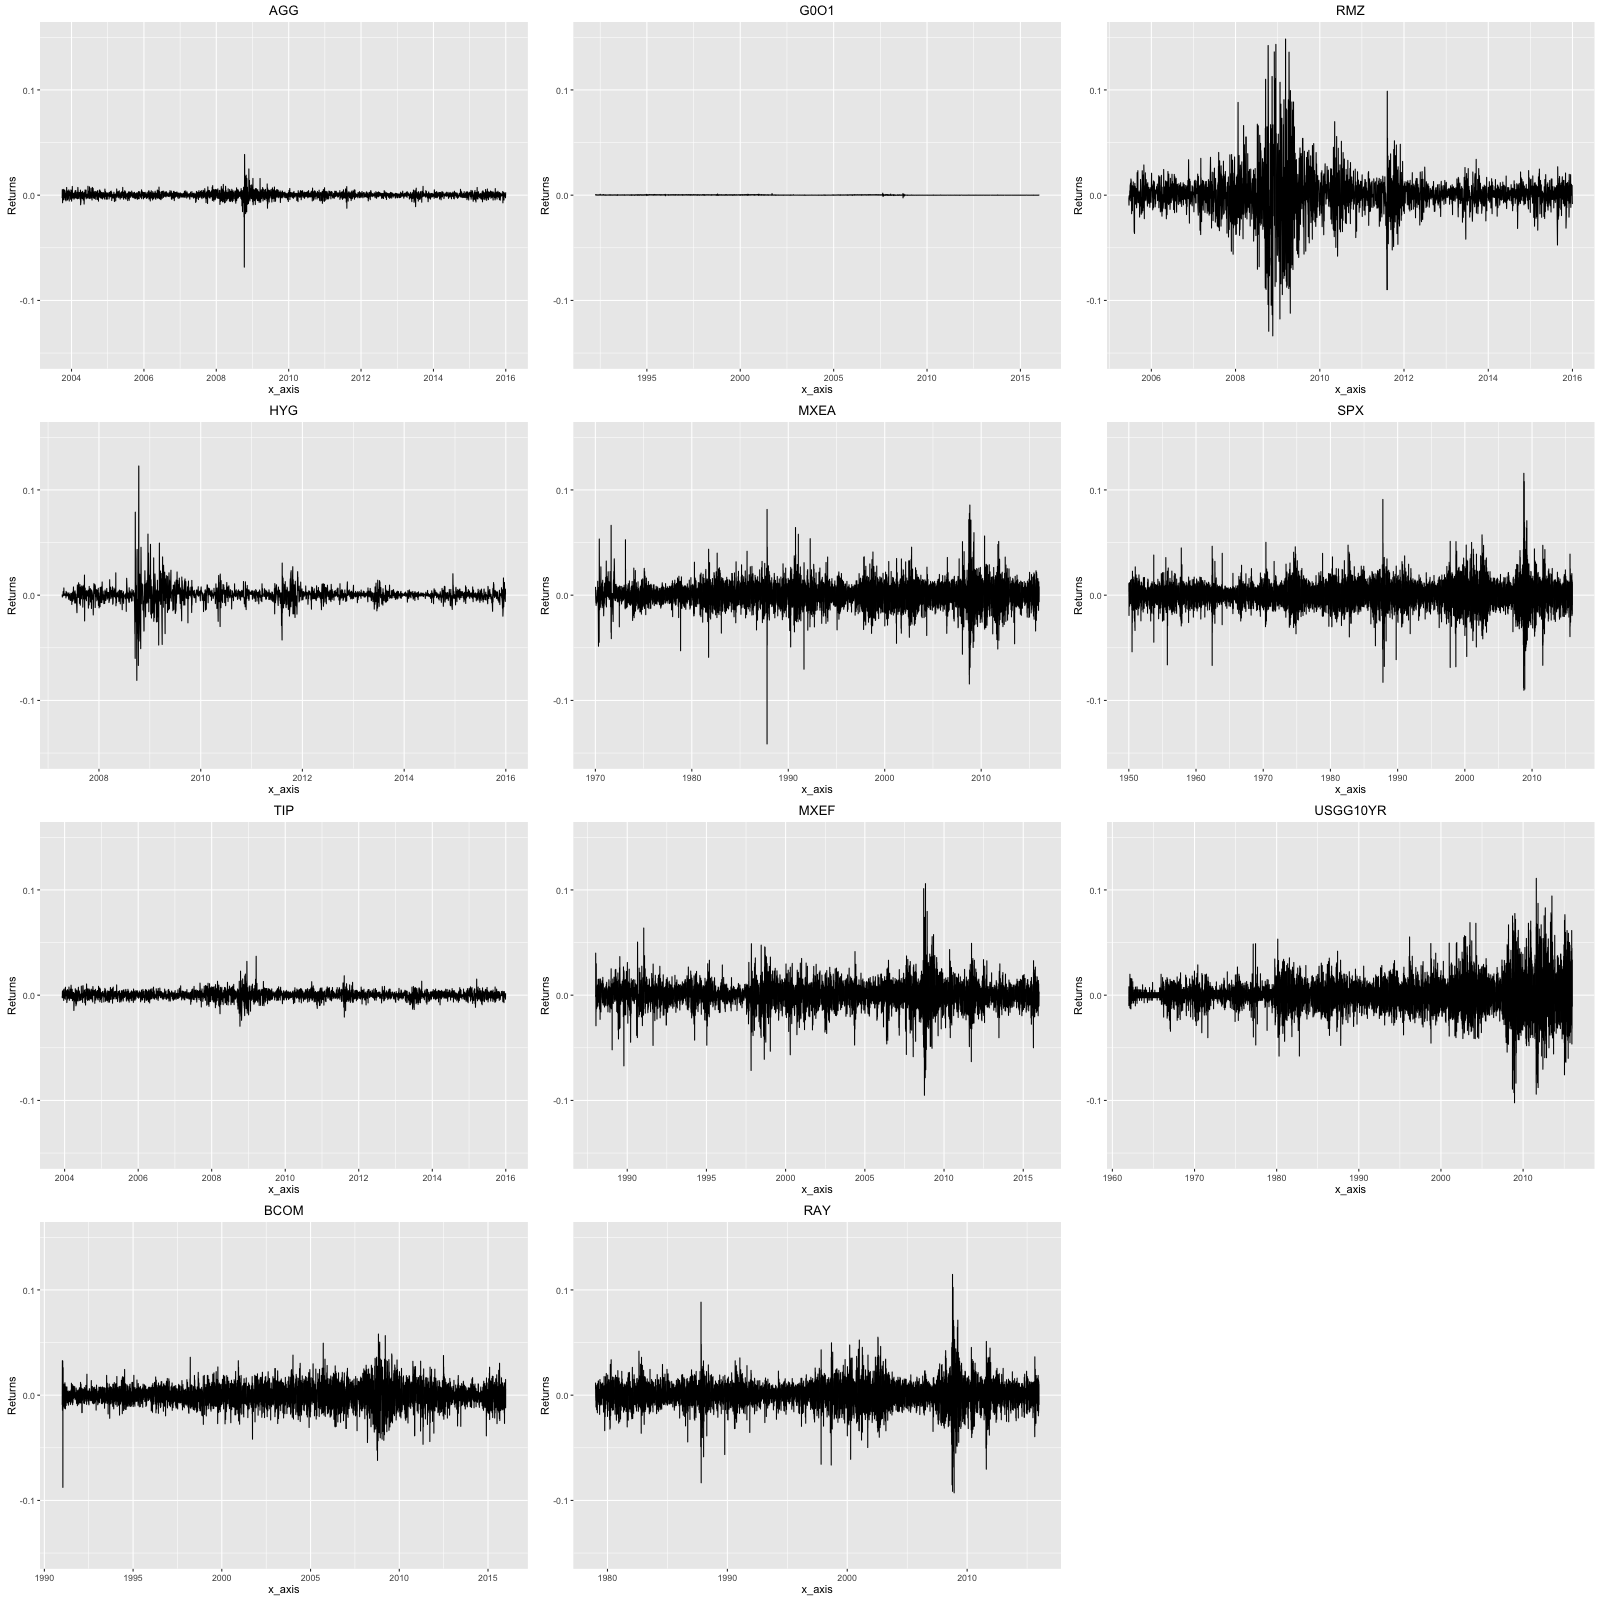
\includegraphics[width=15cm]{../results/returns}
\label{fig: dailyReturns}
\end{figure}

\begin{figure}[h]
\caption{Empirical distribution of daily returns} 
\centering 
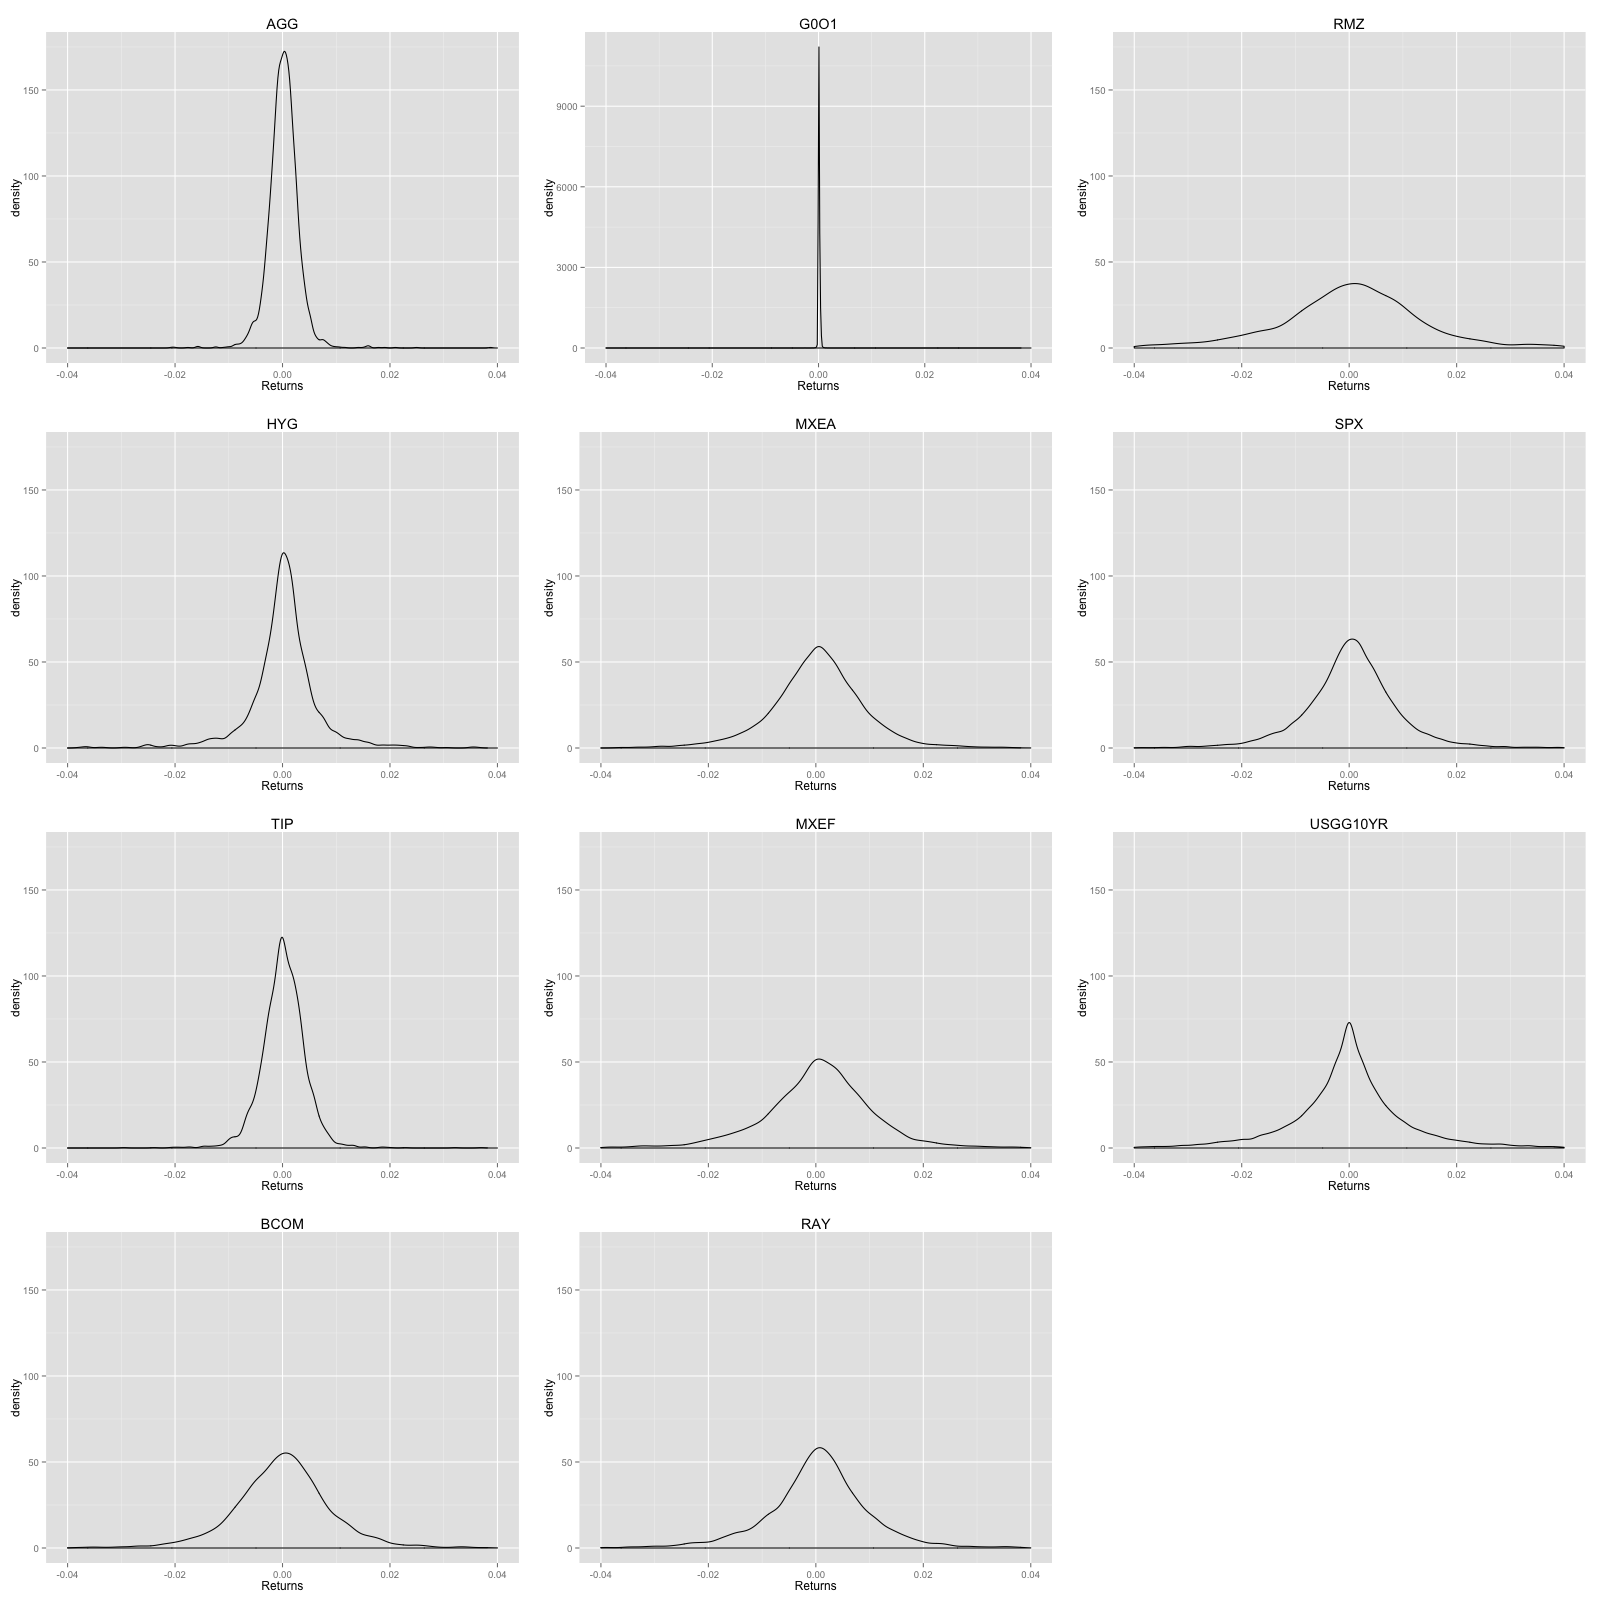
\includegraphics[width=15cm]{../results/returns_dist}
\label{fig: returnsDist}
\end{figure}

\fi
%%%%%%%%

\subsubsection{Statistical summary}

Table \ref{table:statSum} presents the statistical summary of each assets (calculated based on their individual time range). Note that here all asset returns have positive kurtosis (leptokurtic), and nonzero skewness (with both positive and negative values). This is consistent with the Kolmogorov test results in last subsection which show the asset return distribution generally have fat tails.

\begin{table}[!h]
\caption{Statistical Summary of Assets} 
\centering 
\begin{tabular}{ | c || p{1.5cm} p{1.2cm} r r | } 
 \hline
Asset & Sharpe  & Sd. & Skewness & Kurtosis \\
  \hline \hline
AGG & 0.052 & 0.051 & -2.51 & 81.31\\ 
HYG & 0.025 & 0.134 &  0.87 & 36.71\\ 
TIP & 0.040 & 0.065 &  0.10 &  6.48\\ 
BCOM & 0.001 & 0.149 & -0.27 &  4.33\\ 
G0O1 & & 0.002 &  0.69 & 26.76\\ 
MXEA & 0.030 & 0.155 & -0.32 & 10.74\\ 
MXEF & 0.031 & 0.180 & -0.39 &  7.71\\ 
RAY & 0.036 & 0.173 & -0.66 & 17.22\\ 
RMZ & 0.016 & 0.366 &  0.36 & 13.68\\ 
SPX & 0.035 & 0.153 & -0.65 & 21.12\\ 
USGG10YR & 0.003 & 0.201 &  0.12 &  8.81\\
 \hline
\end{tabular}
\label{table:statSum}
\end{table}

%%%%%%%%%%%%%%%%%%%%%
\section{Risk Diagnostics}%%%%%%%%
%%%%%%%%%%%%%%%%%%%%%

In this section, we calculated the risk diagnostics based on the whole available data set of each asset. The value of risk diagnostics increases as the significant level increases.  

\subsection{VaR \& ES}

\begin{itemize}
\item VaR

$\textit{Value at Risk (VaR)}$ is a measure of the risk of investments. It estimates how much a set of investments might lose, given normal market conditions, in a set time period such as a day. VaR is typically used by firms and regulators in the financial industry to gauge the amount of assets needed to cover possible losses. The mathematicial representation of VaR under $\alpha$ was shown below. \footnote{https://en.wikipedia.org/wiki/Value\_at\_risk}
\begin{equation}
VaR_{\alpha}(L) = inf\{l \in \mathbb{R} : P(L > l) \leq 1-\alpha \} = 
inf\{l \in \mathbb{R} : F_L(l) \geq \alpha \}
\end{equation}
\item ES

$\textit{Expected shortfall (ES)}$ is a risk measure -- a concept used in the field of financial risk measurement to evaluate the market risk or credit risk of a portfolio. The ``expected shortfall at q\% level" is the expected return on the portfolio in the worst q\% of cases. ES is an alternative to Value at Risk that is more sensitive to the shape of the loss distribution in the tail of the distribution. The mathematicial representation of ES was shown below.\footnote{https://en.wikipedia.org/wiki/Expected\_shortfall}
\begin{equation}
ES_{\alpha}(L) = E\left[ L \vert L<VaR_{\alpha}(L) \right]
\end{equation}

\end{itemize}

As shown in Table \ref{table:VaRES}, here we calculate the VaR and ES based on different significance levels (0.9, 0.95, 0.99) for various assets. ES is generally bigger than VaR, and the value increases as the significant level increases. RMZ has largest VaR and ES thus the largest risk. AGG, HYG and TIP has smallest VaR and ES thus the smallest risk. 

Note that all the risk diagnostics are calculated based on the empirical distribution of daily returns. Another commonly used method is based on a normal distribution assumption. However, in our case all asset returns have fat tails, it would be rather inappropriate to calculate use normal distribution. Figure \ref{table:VaRESNormal} shows the VaR and ES calculated based on a normal assumption. It turns out VaR and ES is being overestimate at a lower confidence level and being underestimate at a higher confidence level. This discrepancy phenomenon is rather obvious when the return distribution has a fatter tail (a bigger kurtosis).

% https://www.riskprep.com/all-tutorials/37-exam-31/64-var-and-heavy-tails

\begin{table}[!h]
\caption{Empirical VaR and ES under various probabilities} % title of Table
\centering 
\begin{tabular}{ | r || p{1cm} p{1cm} p{1cm} || p{1cm} p{1cm} p{1cm} | } 
 \hline
 & & VaR(\%) &&& ES(\%) & \\
Asset& 0.90 & 0.95 & 0.99 & 0.90 & 0.95 & 0.99 \\
  \hline \hline
AGG & 0.29 & 0.40 & 0.69 & 0.50 & 0.66 & 1.23\\ 
HYG & 0.62 & 1.03 & 2.50 & 1.41 & 2.03 & 4.01\\ 
TIP & 0.44 & 0.62 & 1.01 & 0.72 & 0.91 & 1.47\\ 
BCOM & 1.04 & 1.47 & 2.62 & 1.71 & 2.20 & 3.55\\ 
MXEA & 1.02 & 1.46 & 2.59 & 1.74 & 2.26 & 3.76\\ 
MXEF & 1.21 & 1.76 & 3.32 & 2.11 & 2.75 & 4.67\\ 
RAY & 1.11 & 1.62 & 2.97 & 1.95 & 2.56 & 4.42\\ 
RMZ & 1.91 & 3.00 & 7.56 & 3.99 & 5.62 & 9.99\\ 
SPX & 0.99 & 1.43 & 2.58 & 1.71 & 2.23 & 3.80\\ 
USGG10YR & 1.26 & 1.95 & 3.59 & 2.28 & 2.99 & 4.89\\
 \hline
\end{tabular}
\label{table:VaRES}
\end{table}

\begin{table}[!h]
\caption{Normal VaR and ES under various probabilities} % title of Table
\centering 
\begin{tabular}{ | r || p{1cm} p{1cm} p{1cm} || p{1cm} p{1cm} p{1cm} | } 
 \hline
 & & VaR(\%) &&& ES(\%) & \\
Asset& 0.90 & 0.95 & 0.99 & 0.90 & 0.95 & 0.99 \\
  \hline \hline
AGG & 0.39 & 0.51 & 0.72 & 0.57 & 0.67 & 0.86\\ 
HYG & 1.06 & 1.36 & 1.94 & 1.50 & 1.76 & 2.26\\ 
TIP & 0.51 & 0.66 & 0.94 & 0.74 & 0.86 & 1.11\\ 
BCOM & 1.20 & 1.54 & 2.18 & 1.65 & 1.94 & 2.50\\ 
MXEA & 1.22 & 1.57 & 2.24 & 1.74 & 2.04 & 2.62\\ 
MXEF & 1.42 & 1.83 & 2.61 & 2.03 & 2.38 & 3.06\\ 
RAY & 1.36 & 1.75 & 2.49 & 1.95 & 2.29 & 2.94\\ 
RMZ & 2.92 & 3.75 & 5.32 & 4.08 & 4.79 & 6.18\\ 
SPX & 1.21 & 1.57 & 2.22 & 1.73 & 2.03 & 2.61\\ 
USGG10YR & 1.62 & 2.08 & 2.95 & 2.23 & 2.62 & 3.39\\
 \hline
\end{tabular}
\label{table:VaRESNormal}
\end{table}


%%%%%%%%%%%%%%%%%%%%%
\section{Time Varying Risk Diagnostics}%%
%%%%%%%%%%%%%%%%%%%%%

In this section, we calculate the time varying risk measures, which means to calculate risk measures based on rolling windows, such as 3 month rolling window. Then we get a series of risk measure. By examine how the series of risk measures vary over-time, we may discover some interesting facts about different risk measures.

\subsection{Time varying maximum drawdown}

$\textit{Maximum drawdown}$ is the largest cumulative loss from peak to trough. In the return path of length n, the maximum drawdown is defined by
\begin{equation}
\mathbf{\mu}(X_{T_n}) = \mathrm{max_{1 < i < j \leq n} max}({X_{t_i}-X_{t_j}, 0})
\end{equation}

Unlike VaR and ES, the empirical distribution of maximum drawdown is more sensitive to the time length of measurement. We calculate the maximum drawdown of various assets for different path length (3 months, 6 months, 1 year, 2 years, 5 years) separately. As shown in Figure \ref{fig: dmaxdd_RMZ}, the maximum drawdown distribution tends to be multi-mode and centered around several specific values when we move to longer period. And the mean increases as the period length increases. Figure \ref{fig: dist_mdd} shows the empirical distribution of maximum drawdown under 6 month rolling window for various assets. The maximum drawdown distribution tends to be negative skewed and the density curves seems to be unsmooth even under short rolling period as 6 month. Table \ref{table:tail_maxdrawdown} shows the tail mean of maximum drawdown distributions under different significant levels. Note that the tail mean of maximum drawdown increases as the rolling window increases.

%%%%%%%
\iffalse

\begin{figure}[h]
\caption{Empirical distribution of maximum drawdown under 6 month rolling window} 
\centering
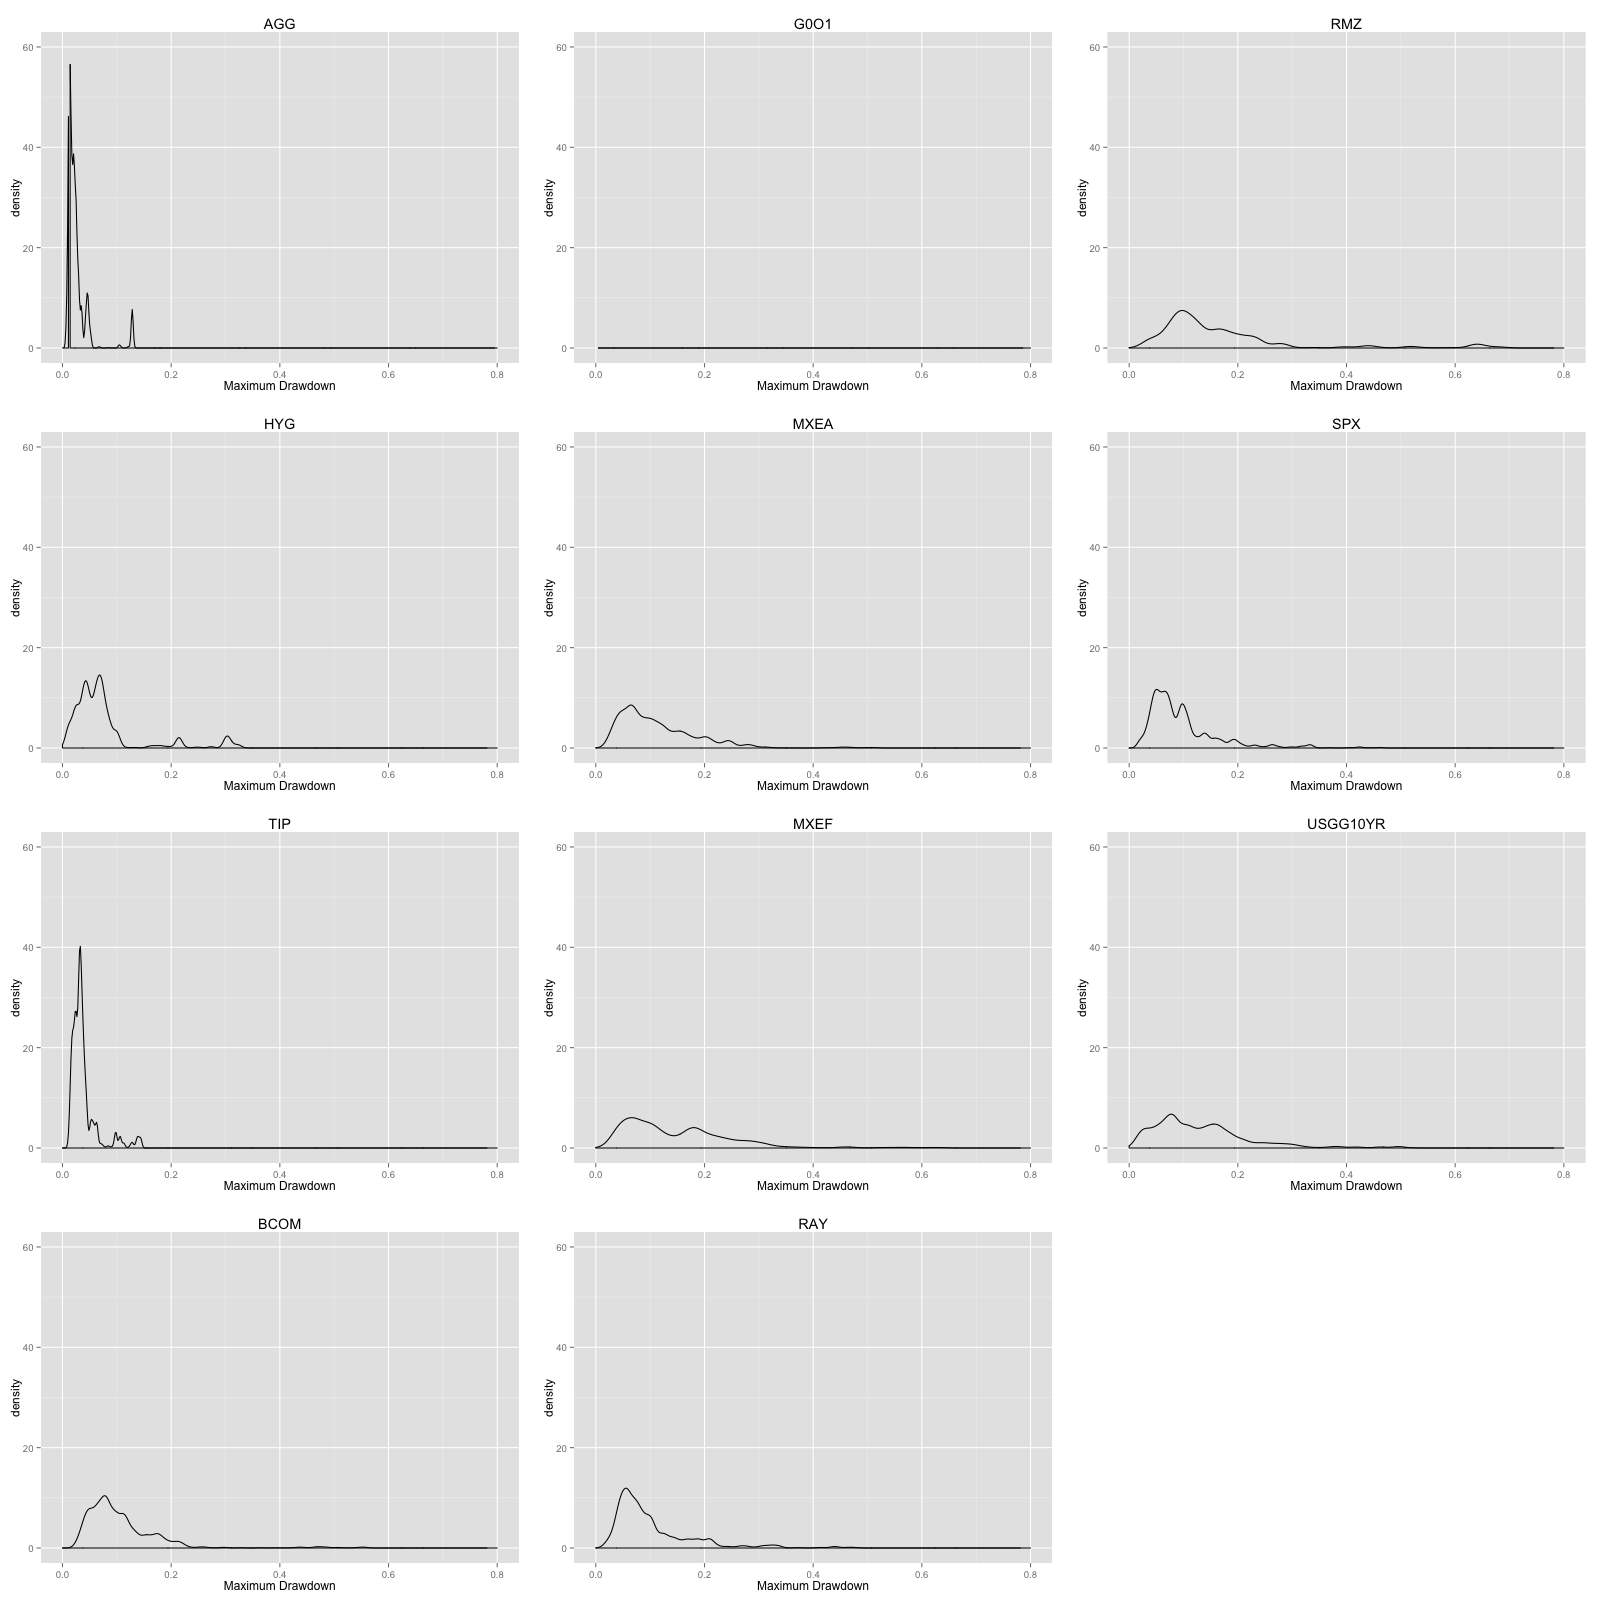
\includegraphics[width=15cm]{../results/maxdd_dist_mon6}
\label{fig: dist_mdd}
\end{figure}

\fi
%%%%%%%

\begin{figure}[h]
\caption{Maximum drawdown distribution of RMZ as rolling period increases} 
\centering 
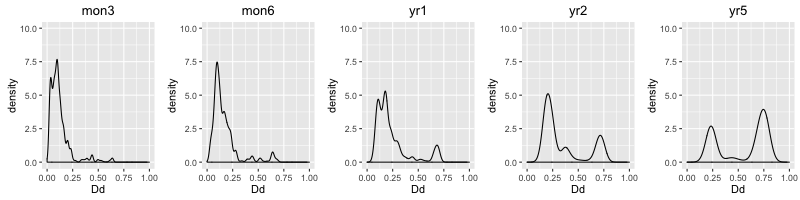
\includegraphics[width = 1\textwidth]{../results/maxdd_RMZ}
\label{fig: dmaxdd_RMZ}
\end{figure}

%%%%%%%
\iffalse

\begin{table}[!h]
\centering 
\caption{tail mean of maximum drawdown distribution under 3-month, 6-month, 1-year and 2-year rolling window} 
\begin{tabular}{ | r || r r r || r r r |} 
 \hline
 & & 3 month & & & 6 month & \\
Asset& 0.9 & 0.95 & 0.99 & 0.9 & 0.95 & 0.99  \\
  \hline \hline
AGG &  5.60 &  7.72 & 12.84 &  8.12 & 11.45 & 12.84\\ 
HYG & 18.41 & 24.07 & 29.67 & 26.43 & 30.77 & 32.26\\ 
TIP &  7.48 &  9.90 & 13.10 & 11.14 & 12.91 & 14.39\\ 
BCOM & 18.14 & 22.54 & 38.03 & 26.61 & 33.66 & 51.74\\ 
G0O1 &  0.10 &  0.145 &  0.26 &  0.14 &  0.23 &  0.26\\ 
MXEA & 20.39 & 23.73 & 33.32 & 27.21 & 31.79 & 47.11\\ 
MXEF & 26.21 & 30.80 & 48.03 & 36.35 & 43.30 & 59.63\\ 
RAY & 20.65 & 25.64 & 35.95 & 27.81 & 34.08 & 45.08\\ 
RMZ & 37.30 & 48.41 & 63.45 & 52.04 & 62.41 & 67.61\\ 
SPX & 18.35 & 22.67 & 32.46 & 25.18 & 30.65 & 40.69\\ 
USGG10YR & 23.28 & 28.11 & 41.83 & 32.78 & 39.00 & 49.28\\
 \hline \hline
 & & 1 year & & & 2 year & \\
Asset& 0.9 & 0.95 & 0.99 & 0.9 & 0.95 & 0.99  \\
  \hline \hline
AGG & 12.11 & 12.84 & 12.84 & 12.84 & 12.84 & 12.83\\ 
HYG & 33.15 & 34.20 &      & 34.24 & 34.25 &       \\ 
TIP & 13.73 & 14.50 & 14.57 & 14.57 & 14.57 &       \\ 
BCOM & 39.91 & 49.26 & 57.14 & 53.38 & 57.14 &       \\ 
G0O1 &  0.23 &  0.25 &  0.26 &  0.26 &  0.26 &  0.26\\ 
MXEA & 36.15 & 42.61 & 56.70 & 50.21 & 58.08 & 61.85\\ 
MXEF & 48.63 & 58.81 & 64.56 & 62.45 & 65.90 &       \\ 
RAY & 37.56 & 44.06 & 52.42 & 47.95 & 54.33 &       \\ 
RMZ & 67.09 & 69.86 & 70.02 & 73.70 & 74.56 & 74.92\\ 
SPX & 34.07 & 39.15 & 50.30 & 44.62 & 50.47 & 56.77\\ 
USGG10YR & 42.88 & 48.37 & 53.96 & 54.79 & 59.14 & 62.82\\
 \hline
\end{tabular}
\label{table:tail_maxdrawdown}
\end{table}

\fi
%%%%%%%

\subsection{Time varying volatility, VaR and ES}

Figure \ref{fig: variance6mon}, \ref{fig: VaR6mon} and \ref{fig: ES6mon} show the time varying volatility, VaR and ES based on 6-month rolling window (significance level = 0.95) for different assets. For every single asset, three risk measures seems to have similar pattern with each other. We further look at this similarity by calculate the correlation between different risk measures.

%%%%%%%
\iffalse

\begin{figure}[h]
\caption{Volatility under 6-month rolling window} 
\centering 
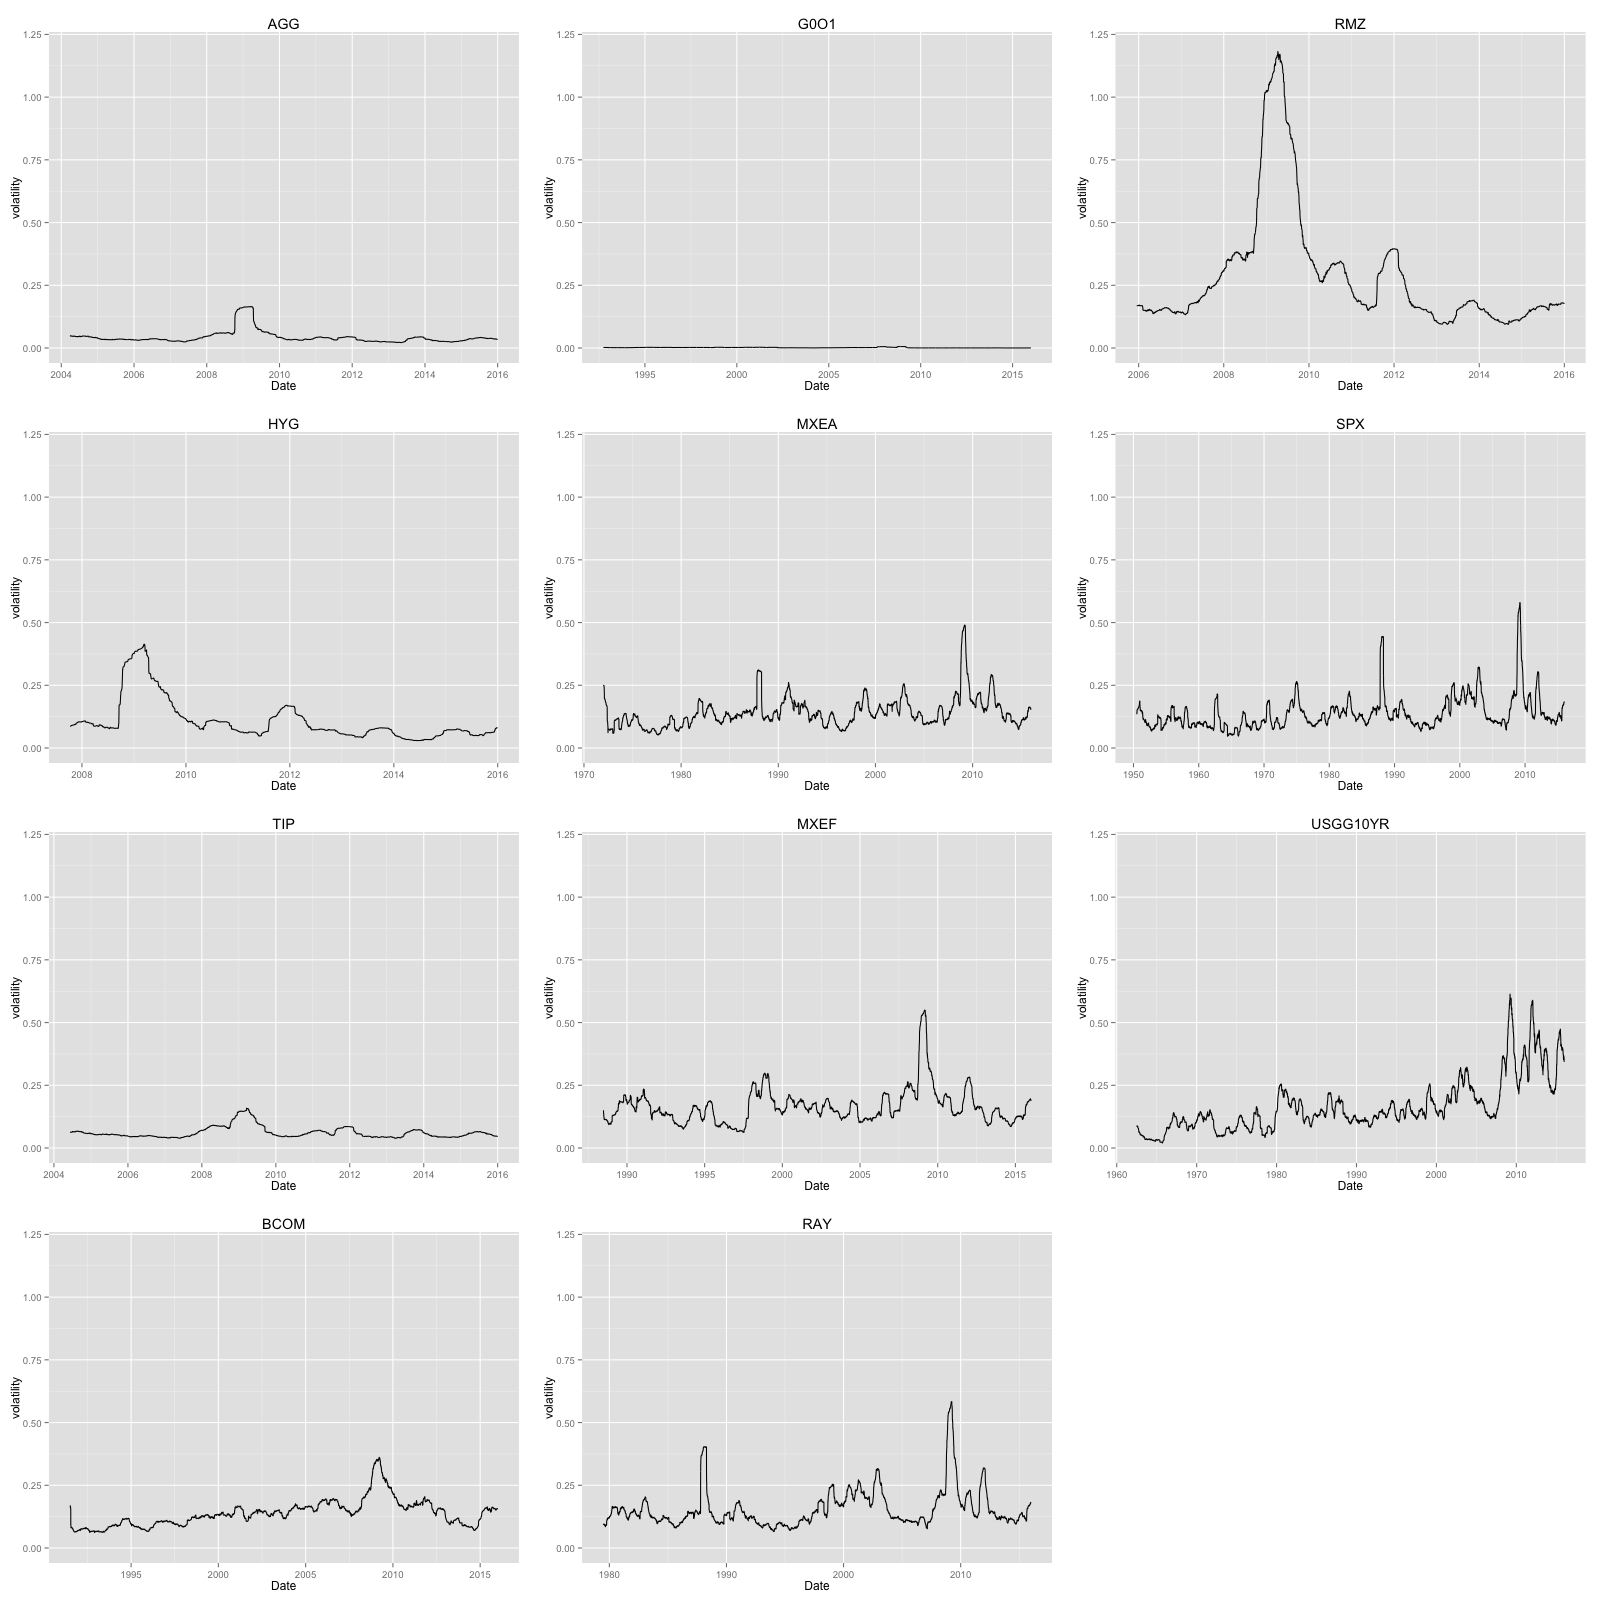
\includegraphics[width=15cm]{../results/volatility6mon}
\label{fig: variance6mon}
\end{figure}

\begin{figure}[h]
\caption{VaR(\%) (significance level = 0.95) under 6-month rolling window}
\centering 
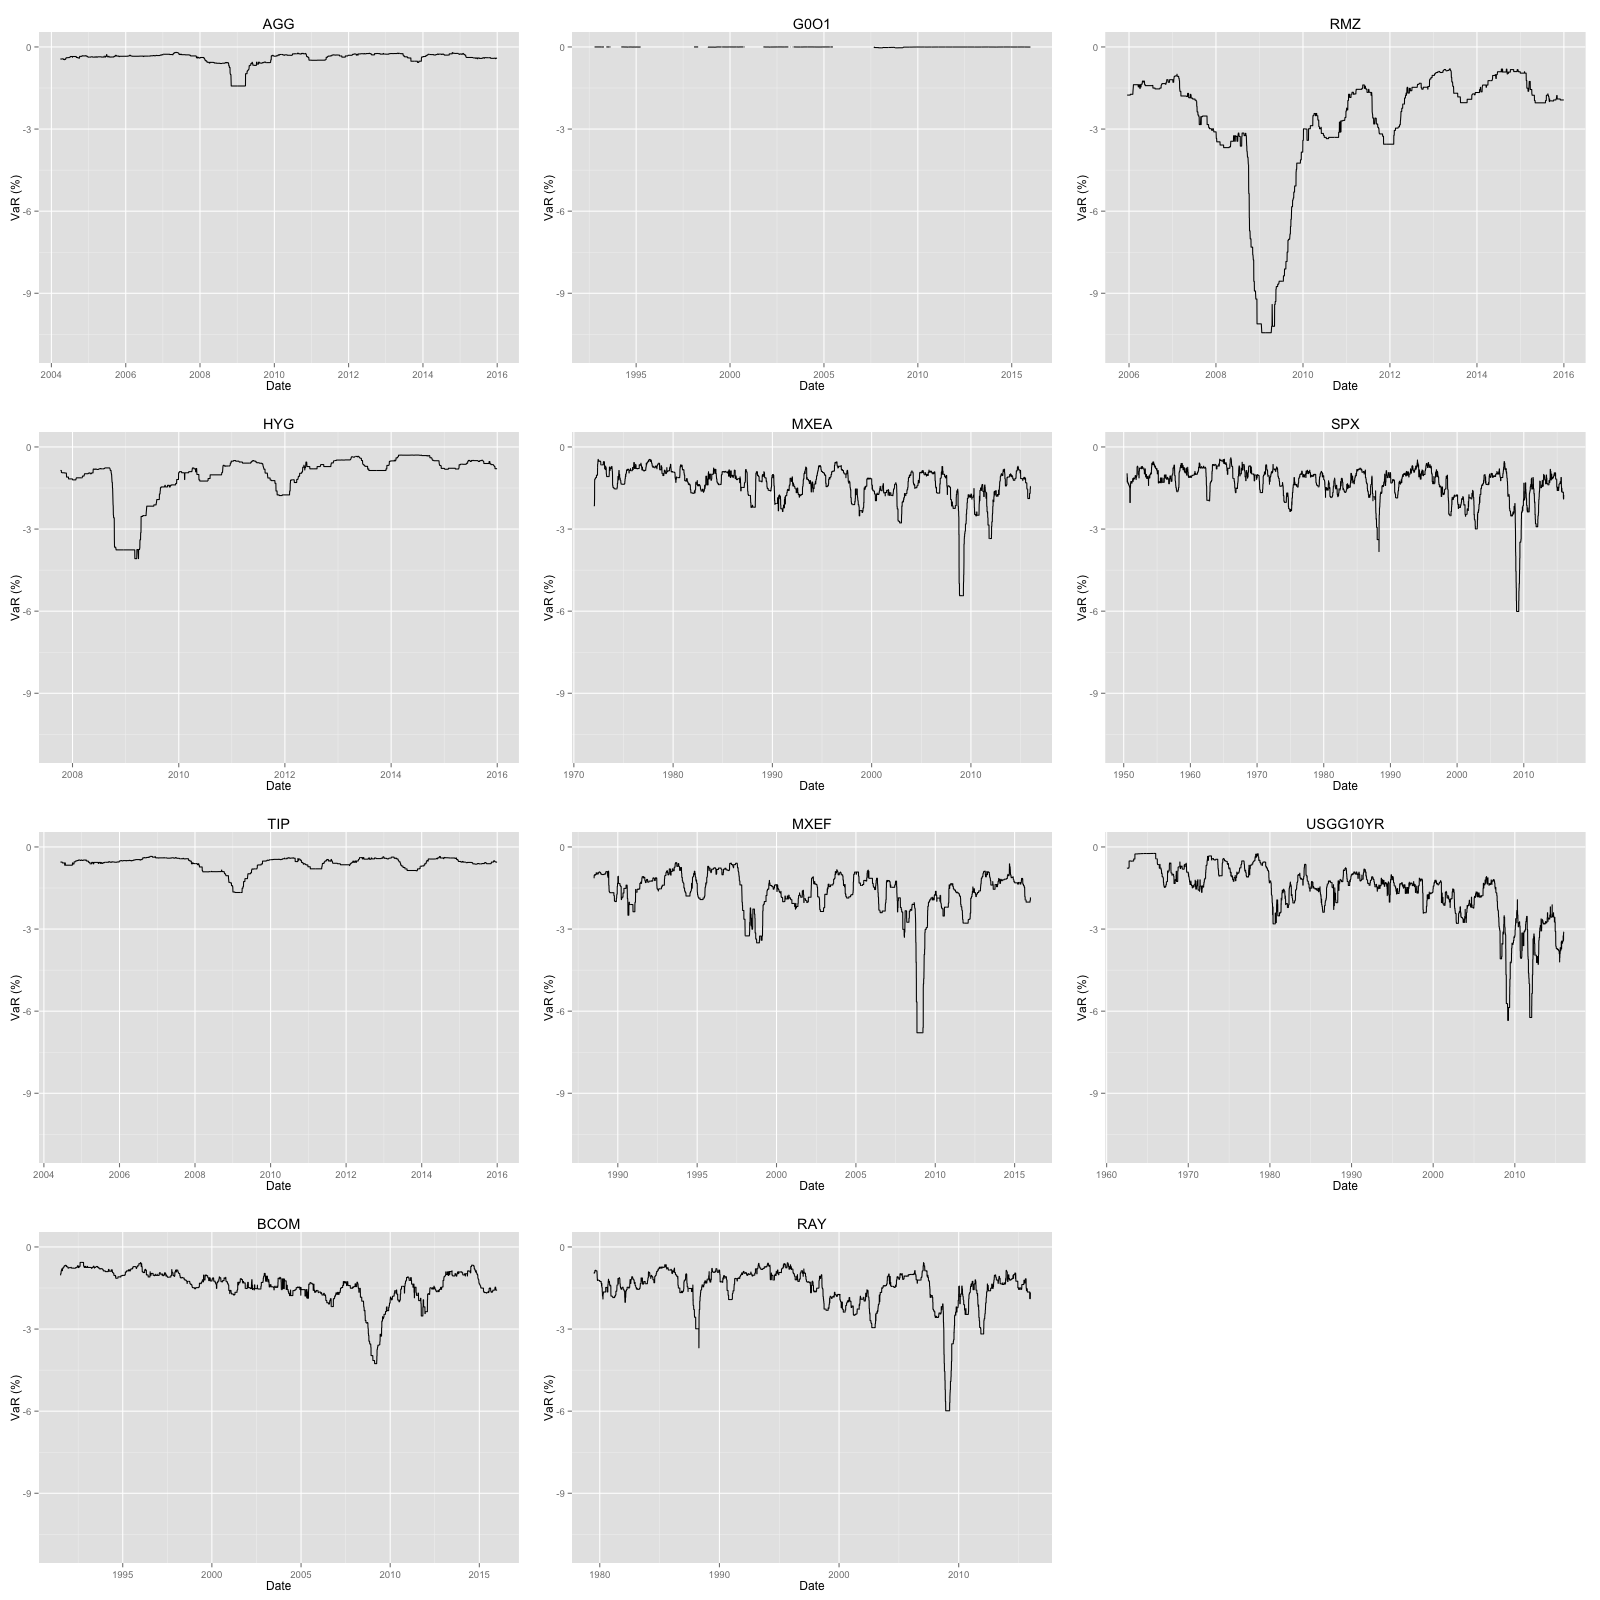
\includegraphics[width=15cm]{../results/VaR6mon_scaled}
\label{fig: VaR6mon}
\end{figure}

\begin{figure}[h]
\caption{ES(\%) (significance level = 0.95) under 6-month rolling window} 
\centering 
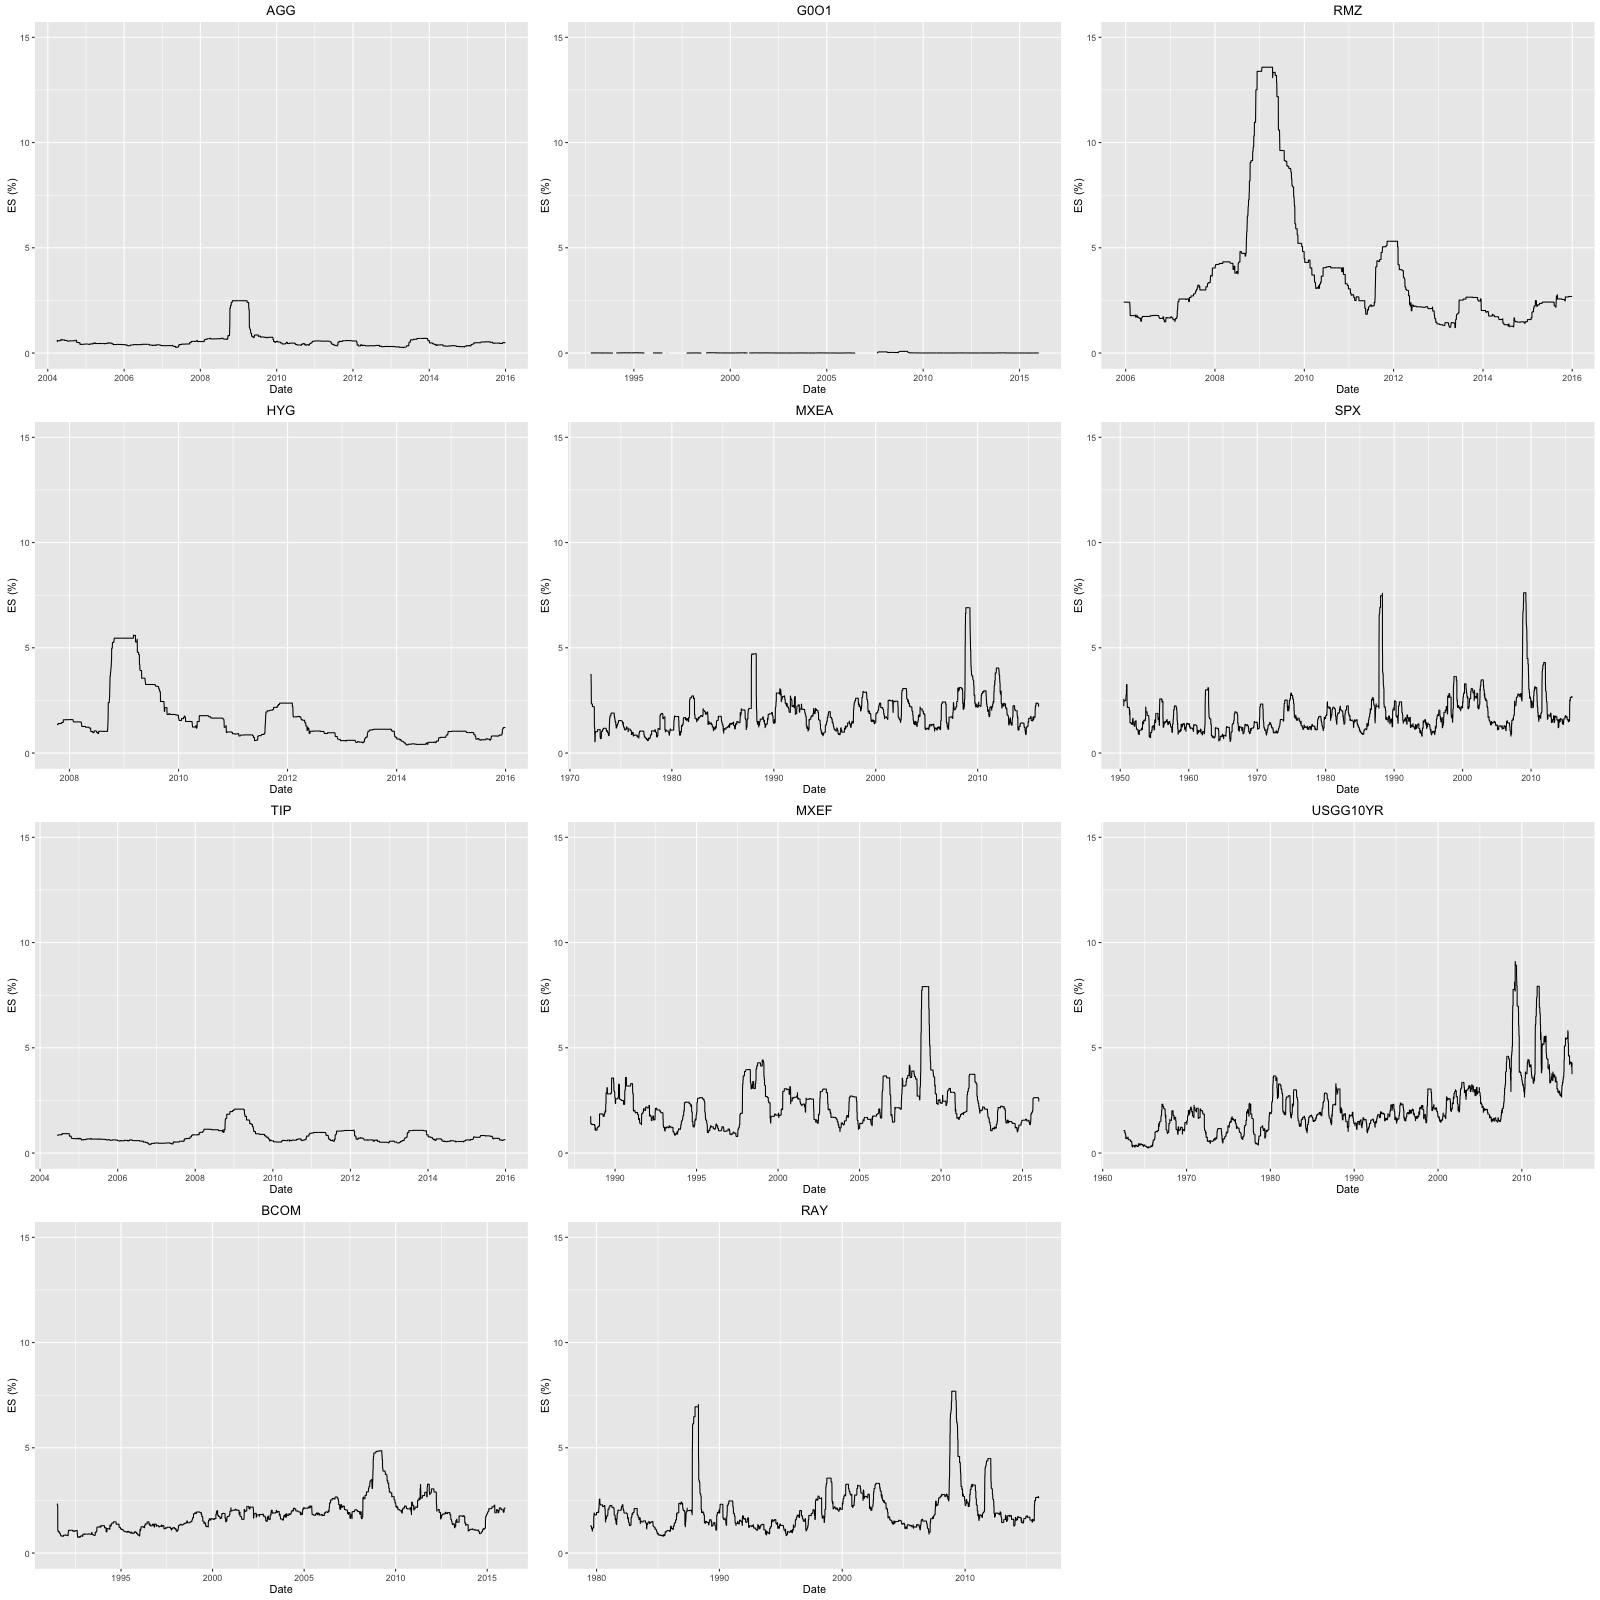
\includegraphics[width=15cm]{../results/ES6mon_scaled}
\label{fig: ES6mon}
\end{figure}

\fi
%%%%%%%

Table \ref{table:corrRiskMeasure} shows correlation between each pair of risk measures including VaR ($\alpha = 0.95$), ES ($\alpha = 0.95$), volatility and maximum drawdown. The correlation is calculated based on 6-month rolling risk measures. Among them, VaR, ES and volatility are closely related with each other, with average correlations over 95\%. Maximum drawdown has strong but comparatively weaker correlation with the other three. In general, these risk measures are all closely correlated. Figure \ref{fig: risk_meausre_RMZ} shows the comparison of the four risk measures calculated based on rolling windows for asset RMZ. Their pattens turned out to be very similar.

\begin{table}[h]
\caption{Correlation between risk measures}
\centering 
\begin{tabular}{ p{2cm}||p{1.6cm}|p{1.6cm}|p{1.6cm}|p{1.6cm}|p{1.6cm}|p{1.6cm}} 
\hline
Measure 1 & \multicolumn{3}{|c|}{Maximum drawdown} & \multicolumn{2}{|c|}{Volatility} & VaR\\ \hline
Measure 2 & Volatility & VaR & ES & VaR & ES & ES\\
  \hline \hline
AGG & 0.90 & 0.89 & 0.94 & 0.96 & 0.98 & 0.95\\ 
HYG & 0.95 & 0.95 & 0.96 & 0.99 & 0.99 & 0.99\\ 
TIP & 0.72 & 0.82 & 0.83 & 0.94 & 0.97 & 0.96\\ 
BCOM & 0.67 & 0.76 & 0.74 & 0.96 & 0.96 & 0.96\\
MXEA & 0.76 & 0.82 & 0.80 & 0.94 & 0.97 & 0.94\\ 
MXEF & 0.79 & 0.86 & 0.86 & 0.96 & 0.97 & 0.97\\ 
RAY & 0.87 & 0.85 & 0.87 & 0.96 & 0.96 & 0.92\\ 
RMZ & 0.90 & 0.92 & 0.93 & 0.99 & 0.99 & 0.99\\ 
SPX & 0.80 & 0.80 & 0.80 & 0.96 & 0.96 & 0.93\\ 
USGG10YR & 0.77 & 0.84 & 0.83 & 0.97 & 0.97 & 0.98\\ 
\hline
\end{tabular}
\label{table:corrRiskMeasure}
\end{table}

\begin{figure}[h]
\caption{Comparison of different risk measures of RMZ} 
\centering 
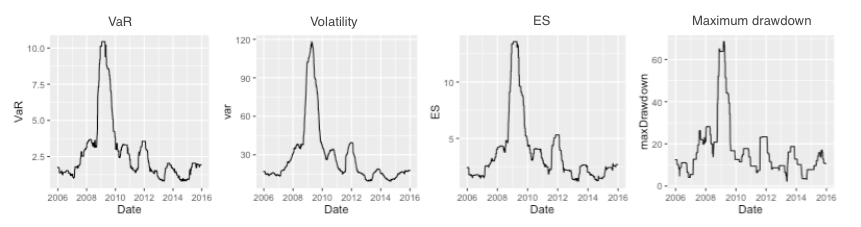
\includegraphics[width = 1\textwidth]{../results/risk_measure_RMZ}
\label{fig: risk_meausre_RMZ}
\end{figure}


\subsection{Time varying CED}

Maximum drawdown is the largest cumulative loss from peak to trough. Conditional Expected Drawdown (CED) is the tail mean of maximum drawdown distributions.\footnote{On a Convex Measure of Drawdown Risk. Lisa R. Goldberg, Ola Mahmoud} Under confidence level $\alpha$, the conditional expected drawdown is defined as:
\begin{equation}
CED_\alpha(X_{T_n}) = \textbf{E}(\mathbf{\mu}(X_{T_n})|\mathbf{\mu}(X_{T_n}) > DT_\alpha)
\end{equation}
where $\mathbf{\mu}(X_{T_n})$ is the maximum drawdown distribution over a finite path.

Here we calculated the CED using a 3-month-2-year rolling window (Figure \ref{fig: CED3mon2yr}).  Note that here we use 3 month as the basic period. For empirical distribution of 3-month maximum drawdown, there are less multi-mode problems, and the tail value is more informative than using longer period. For longer path length such as 2-year and 5-year, there might be some missing values under large confidence levels. CED data tend to be lack of variance under long time period. In such cases, the empirical quantile no longer exits without some distribution or polynomial assumption of the tail. Since we do not familiar the performance of CED, it becomes impropriate to make such assumptions. 

%%%%%
\iffalse

\begin{figure}[h]
\caption{CED under 3-month-5-year Rolling Window (confidence level = 0.95)} 
\centering 
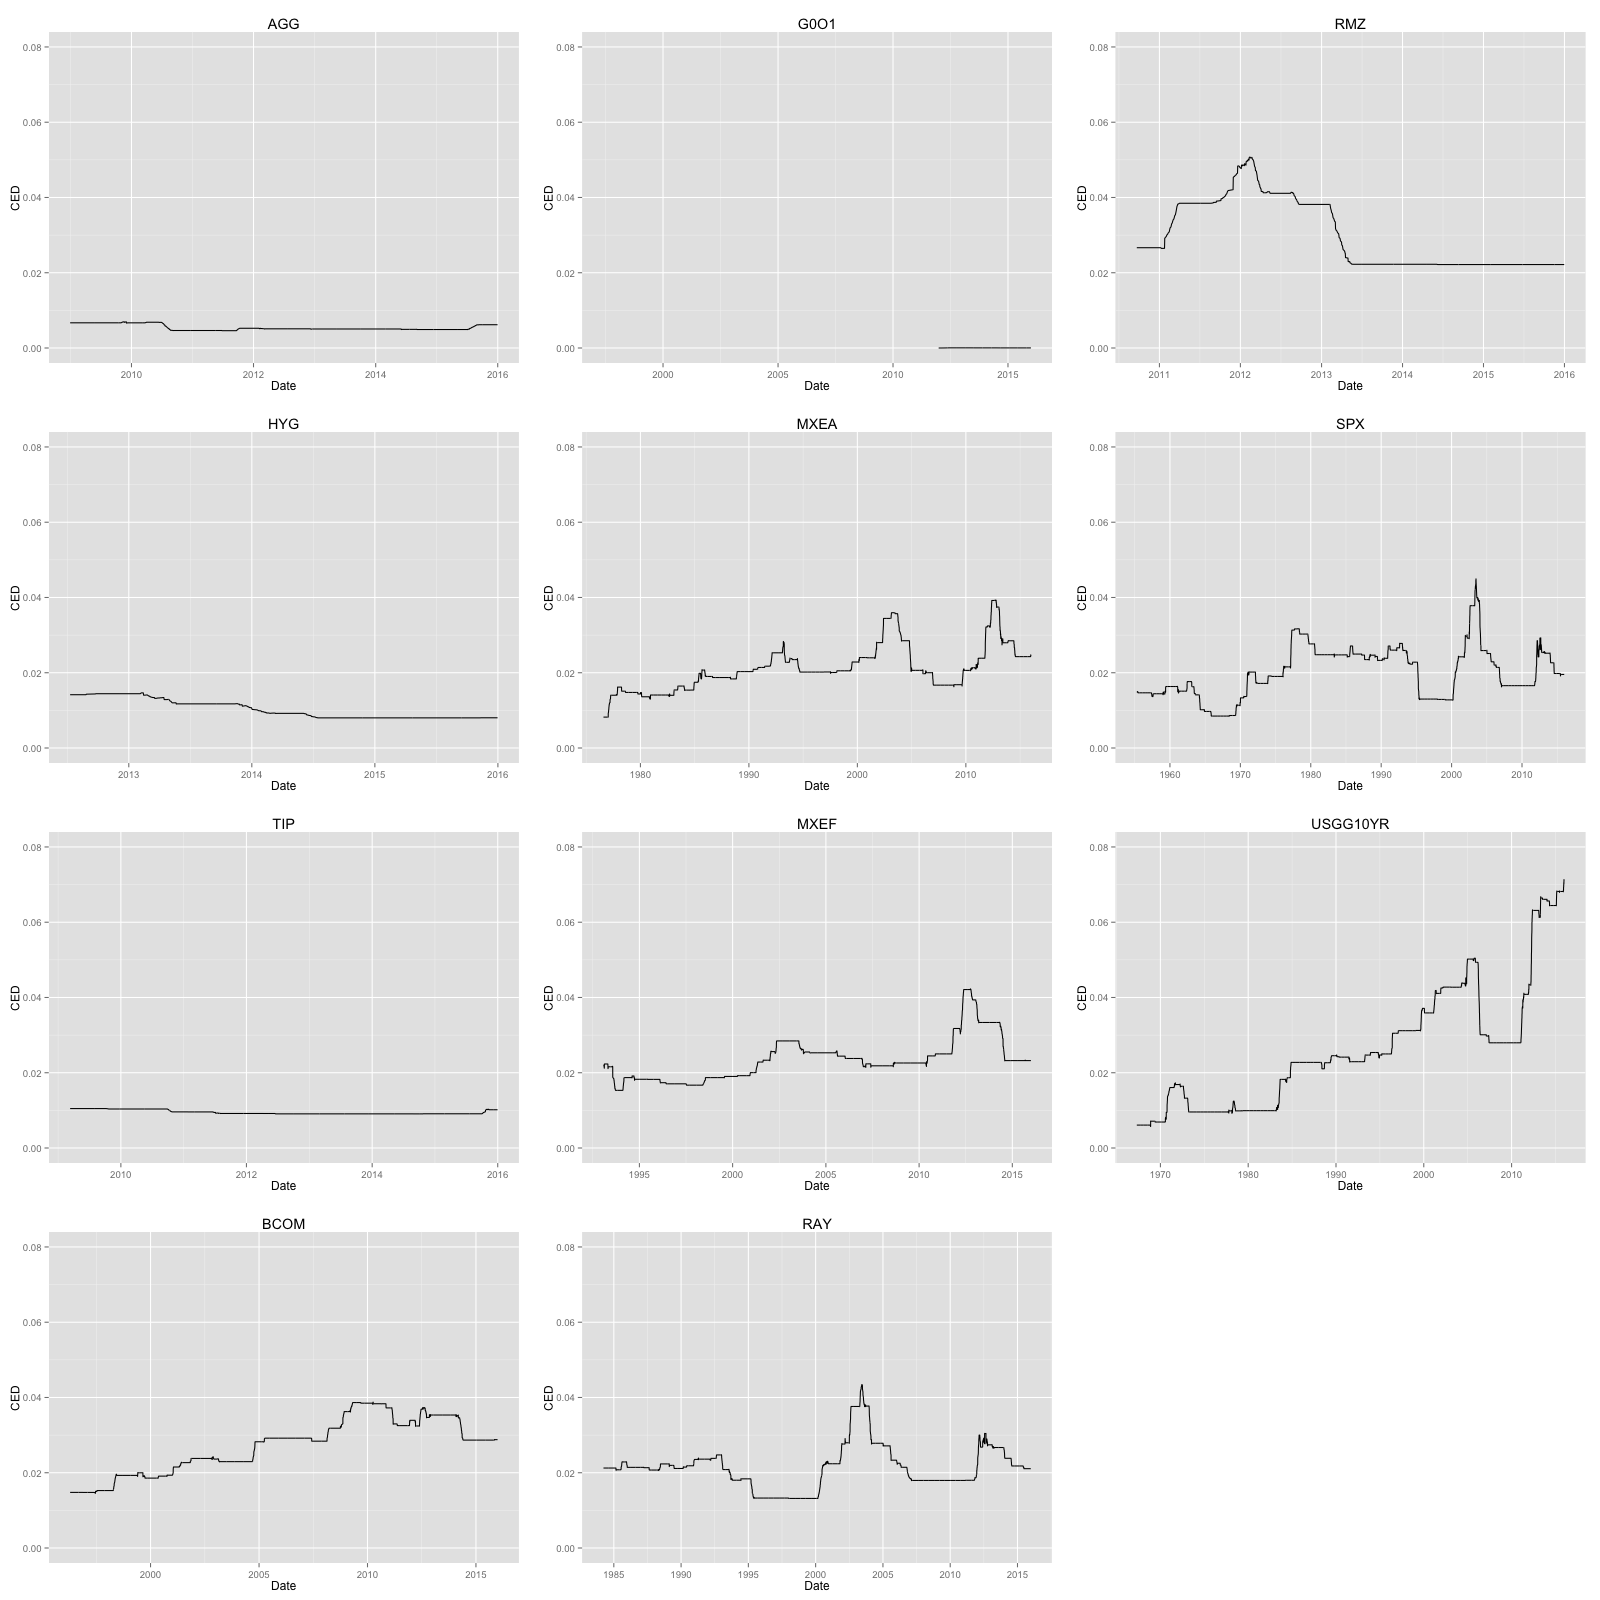
\includegraphics[width=15cm]{../results/CED_3mon_5yr_95}
\label{fig: CED3mon5yr95}
\end{figure}

\fi
%%%%%%

CED is also closely related with other traditional risk measure. However, the correlation between CED and the other three risk measures are slightly weaker than the correlation among volatility, VaR and ES. Table \ref{table:corrRiskMeasureCED} shows the correlation between CED and other risk measures. Again, the correlation is calculated based on 6-month rolling risk measures for every asset. Moreover, Figure \ref{fig: CED_ES_3mon_5yr5yr} shows the plot of ES and CED, which indicates their positive correlated relationship.


\begin{table}[!h]
\caption{Correlation between CED (confidence level = 0.9) and other risk measures}
\centering 
\begin{tabular}{ p{2cm}||p{2cm}|p{2cm}|p{2cm}} 
\hline
Measures & Volatility & VaR & ES\\
  \hline
AGG & 0.94 & 0.89 & 0.95\\ 
HYG & 0.98 & 0.97 & 0.97\\ 
TIP & 0.77 & 0.85 & 0.85\\ 
BCOM & 0.84 & 0.89 & 0.89\\ 
MXEA & 0.84 & 0.83 & 0.86\\ 
MXEF & 0.91 & 0.91 & 0.93\\ 
RAY & 0.92 & 0.85 & 0.92\\ 
RMZ & 0.96 & 0.96 & 0.97\\ 
SPX & 0.84 & 0.81 & 0.84\\ 
USGG10YR & 0.91 & 0.93 & 0.95\\
\hline
\end{tabular}
\label{table:corrRiskMeasureCED}
\end{table}

% \subsection{Time varying seirial correlation and their relationship with risk measures}


%%%%%
\iffalse

\begin{figure}[h]
\caption{CED (confidence level = 0.9) versus ES under 3-month-5-year Rolling Window} 
\centering 
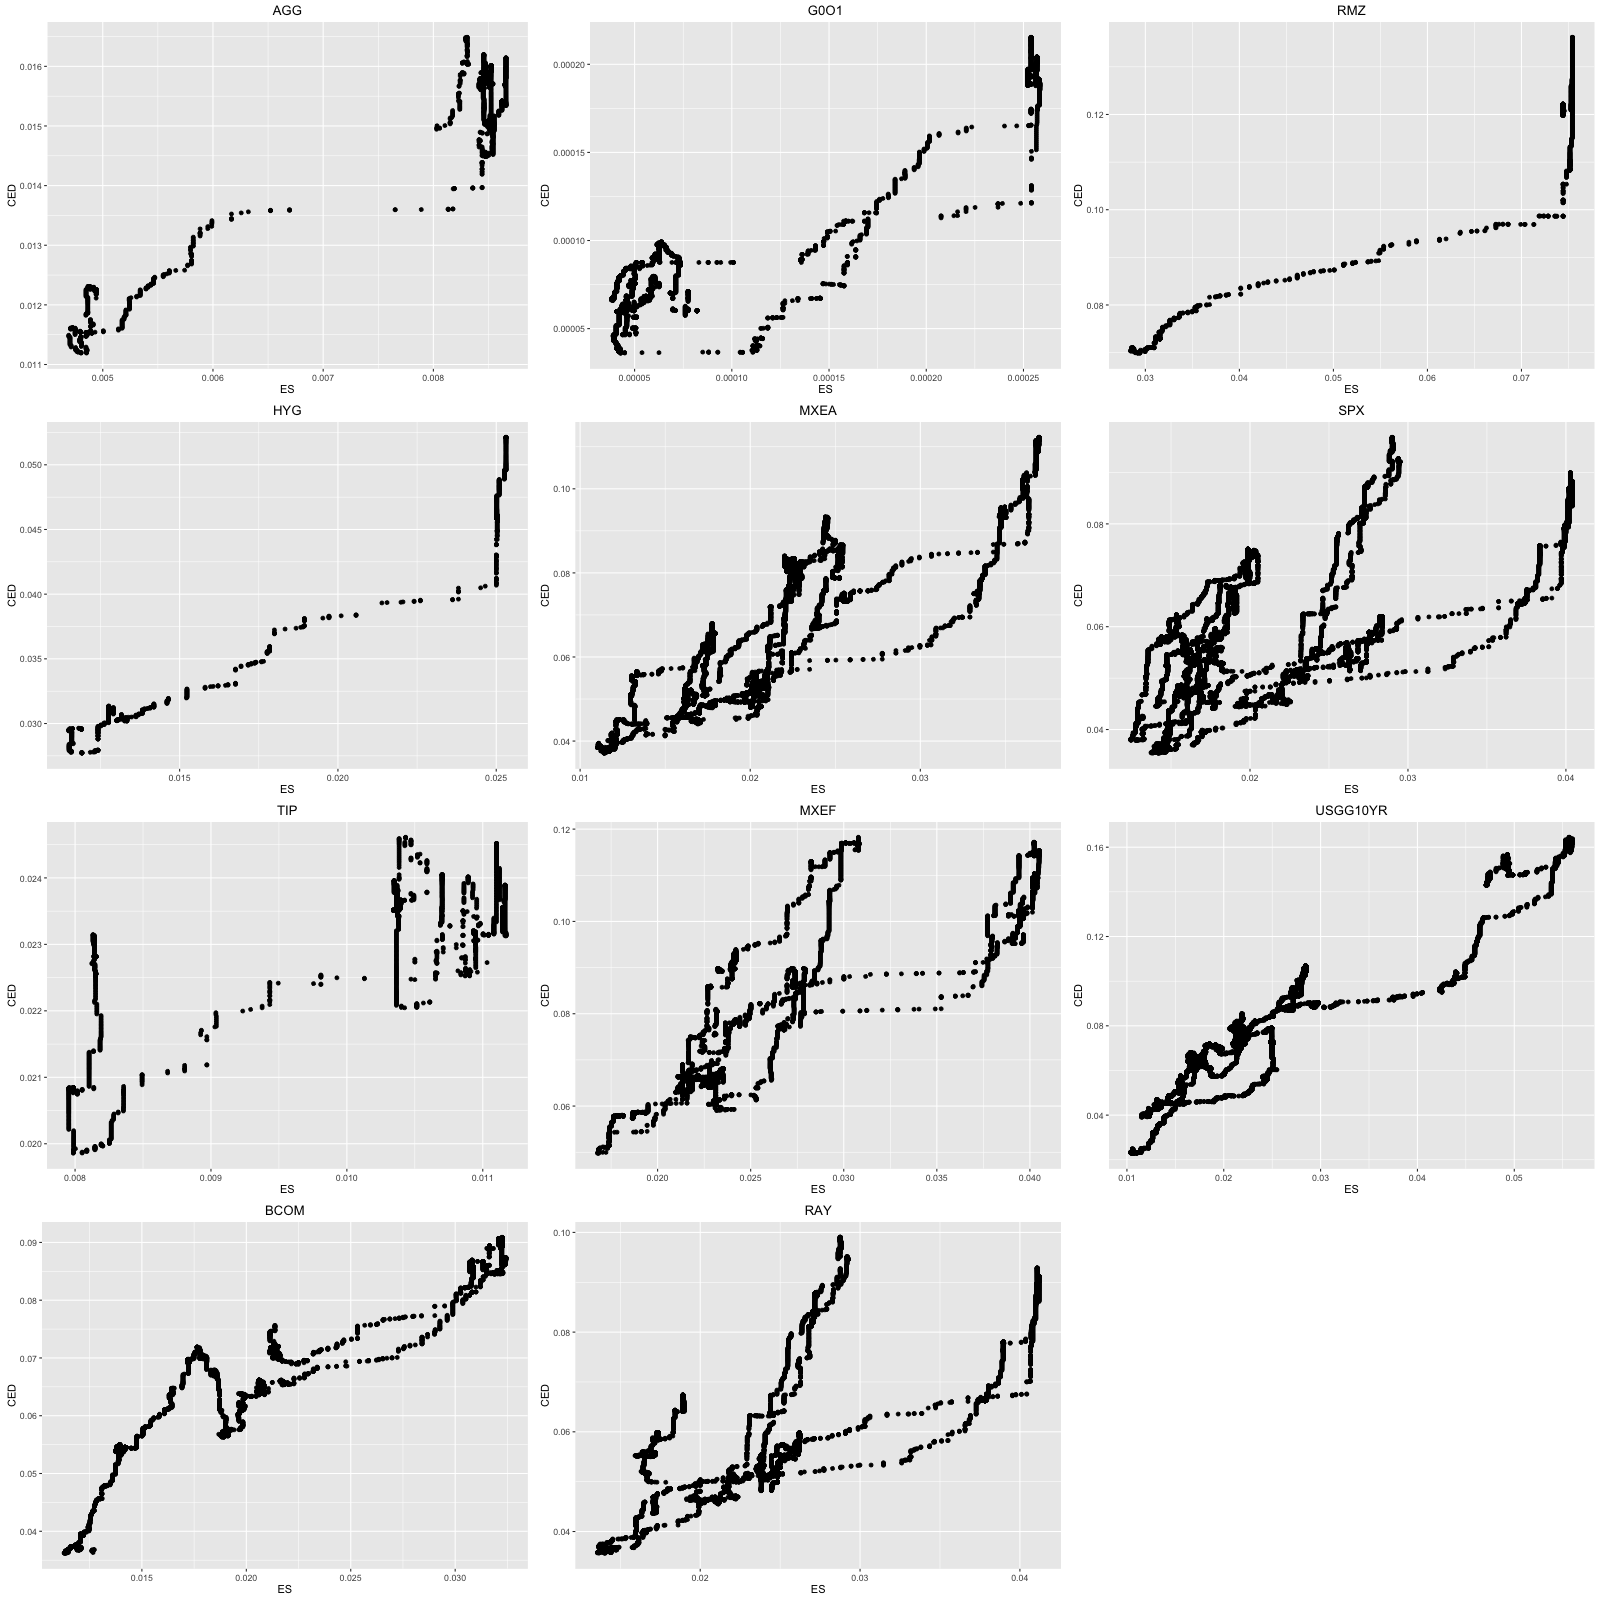
\includegraphics[width=15cm]{../results/CED_ES_3mon_5yr5yr}
\label{fig: CED_ES_3mon_5yr5yr}
\end{figure}

\fi
%%%%%%

%%%%%%%%%%%%%%%%%%%%%
\section{Regime Switching Model}%%%%
%%%%%%%%%%%%%%%%%%%%%

\iffalse
%-*- program: xelatex -*-        
%-*- program: biber -*-`        
%-*- program: xelatex -*-
\documentclass[12pt]{article}
\usepackage{amsmath,textcomp,amssymb,geometry,graphicx,enumerate,upquote,color}
\usepackage{array}
\usepackage[english]{babel}
\begin{document}

\section{Regime Switching Model}
\fi

Many economic time series data tend to behave differently in adjacent time period. For example, asset returns
usually show large volatility during financial crisis. One common approach to model this abrupt change in regime is to use the Hamilton's Markov regime switching model. In our study, we use the following two-regime switching model to fit the returns:

\begin{equation}
y_t - \mu_{s^*_t} = \phi_{s^*_t} (y_{t-1} - \mu_{s^*_{t-1}}) + \epsilon_t
\end{equation}
where the number of autoregressive coefficient is set to 1. $s^*_t$ is a two state Markov chain. $s^*_t = 1$ represent regime 1 and $s^*_t = 2$ represent regime 2. $s^*_t$ depends on the past only through the most recent values:

\begin{equation}
P(s_t = j|s_{t-1}, s_{t-2}, \dots) = P(s_t = j|s_{t-1})  = p_{ij}
\end{equation}

\subsection{Comparison of basic summary of two regimes}

Table \ref{table:autoCoeffRegime} shows the autoregression coefficient $\phi$ of two regimes for various assets. One interesting fact is that asset returns are more likely (6 out of 10 assets) to show positive autocorrelation in low volatility regimes and negative autocorrelation in high volatility regimes.

Table \ref{table:statSumRegime} shows the standard deviation, skewness and kurtosis of various assets in two regimes separately. Note that regime 1 represents high volatility regime while regime 2 represents low volatility regime. In general, it is clear that returns of regime 1 has a larger standard deviation, skewness and kurtosis than that of regime 2. This indicates that the distribution in low volatility regimes are more ``close" to normal distribution. Their mean returns are more close to zero and they have lighter tails than returns of high volatility regime. In contrast, in high volatility regimes, there are more extreme value of returns which means a fatter tail.

\begin{table}[!h]
\caption{$\phi$ of high and low volatility regimes for various assets} 
\centering 
\begin{tabular}{ | c || r  r | } 
 \hline
 & Regime 1  & Regime 2\\
Asset & High volatility  & Low volatility \\
  \hline \hline
AGG  & -0.134 & -0.114 \\ 
HYG & -0.010 &  0.025 \\ 
TIP &  0.039  & -0.026 \\ 
BCOM & -0.046 &  0.050 \\ 
MXEA & 0.095 & 0.109 \\ 
MXEF & 0.221 & 0.254 \\ 
RAY& -0.039  &  0.052 \\ 
RMZ & -0.244 &  0.007 \\ 
SPX & -0.018 &  0.113 \\ 
USGG10YR & -0.031 & 0.082 \\ 
 \hline
\end{tabular}
\label{table:autoCoeffRegime}
\end{table}

\begin{table}[!h]
\caption{Summary statistics of two regimes for various assets} 
\centering 
\begin{tabular}{ | c || rr | rr | rr | } 
 \hline
& \multicolumn{2}{c|}{Volatility} & \multicolumn{2}{c|}{Skewness} & \multicolumn{2}{c|}{Kurtosis} \\
Asset & Regime 1 & Regime 2 & Regime 1 & Regime 2 & Regime 1 & Regime 2 \\
  \hline \hline
AGG & 0.141 & 0.036 & -1.59 &  0.01 & 17.15 &  0.60\\ 
HYG & 0.265 & 0.055 &  0.60 &  0.00 &  8.76 &  0.83\\ 
TIP & 0.113 & 0.049 &  0.18 & -0.06 &  2.50 &  0.16\\ 
BCOM & 0.205 & 0.096 & -0.25 & -0.04 &  1.92 &  0.28\\ 
MXEA & 0.253 & 0.101 & -0.14 & -0.02 &  4.26 &  0.25\\ 
MXEF & 0.303 & 0.119 & -0.08 & -0.06 &  2.39 &  0.38\\ 
RAY & 0.307 & 0.114 & -0.39 & -0.06 &  6.43 &  0.55\\ 
RMZ & 0.661 & 0.159 &  0.29 & -0.15 &  2.92 &  0.79\\ 
SPX & 0.260 & 0.099 & -0.43 & -0.02 &  9.11 &  0.56\\ 
USGG10YR & 0.314 & 0.098 &  0.09 & -0.05 &  2.67 &  1.17 \\
 \hline
\end{tabular}
\label{table:statSumRegime}
\end{table}

\subsection{Detailed analysis (Take RMZ as an example)}

\subsubsection{Summary}

In Figure \ref{fig: RMZregime}, we use RMZ as an example of our volatility regime analysis. The upper panel show the daily returns and their corresponding regimes. The shadowed area represents the regime with high volatility and the white area low volatility. The X axis shows the indices of business days from 06/30/2005 to 12/31/2015. The lower panel shows the smoothed probability of Markov switching model corresponds with the high volatility regime. This model is consistent with the actual financial event in that the high volatility regime covered mainly from mid-2007 to 2010, which is roughly the period of 2008-09 financial crisis.

Table \ref{table:statSumRegimeRMZ} shows the descriptive summary and risk diagnostics for RMZ of each regime. As we might expect, regime with high volatility also shows high risks in that they have larger ES and VaR values. Moreover, model of regime 1 only explains 26.3\% of the observations, which means abrupt deviation is minority in total observations. By looking at assets with longer period, we find a similar proportion of high volatility regimes (SPX: 23.7\%, RAY: 20.6\%).

%\begin{figure}[h]
%\caption{Regime plot of SPX returns and its smoothed probabilities} 
%\centering 
%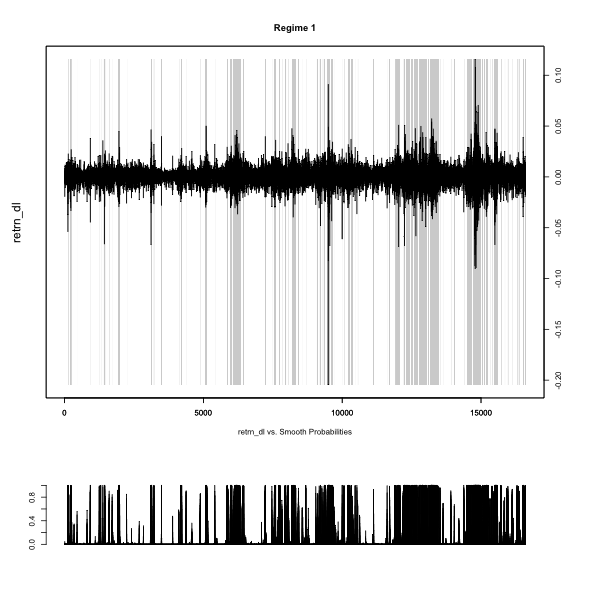
\includegraphics[width=1\textwidth]{../results/regime/SPX}
%\label{fig: returnsDist}
%\end{figure}

\begin{figure}[h]
\caption{Regime plot of RMZ returns and its smoothed probabilities} 
\centering 
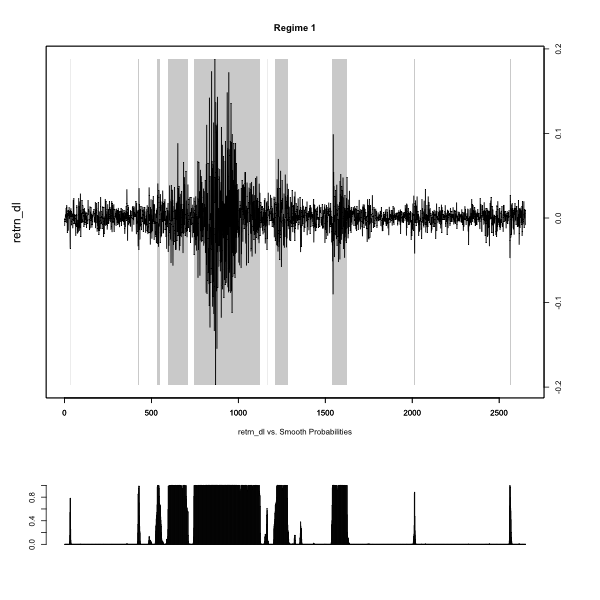
\includegraphics[width=1\textwidth]{../results/regime/RMZ}
\label{fig: RMZregime}
\end{figure}

\begin{table}[!h]
\caption{Descriptive summary and risk diagnostics for RMZ of each regime} 
\centering 
\begin{tabular}{| r | r | r |} 
 \hline
& Regime 1 & Regime 2 \\
& High volatility & Low volatility \\
 \hline 
Mean & -0.046\% & 0.067\% \\
Number of trading days & 699 & 1954\\ 
Percentage of observations & 26.3\% & 73.7\% \\ 
Maximum daily return &18.8\% & 3.6\% \\
Minimum daily return & -19.7\% & -4.0\% \\
Longest continuous days & 381 & 546\\ \hline
VaR (empirical, p = 0.95) & 6.8\% & 1.6\% \\
ES (empirical, p = 0.95) & 9.3\% & 2.2\% \\
 \hline
\end{tabular}
\label{table:statSumRegimeRMZ}
\end{table}

\subsubsection{Risk diagnostics}

In order to make a consistent comparison of risk diagnostics between two regimes, we ignore some short discontinuity and pick two longest single occurring episode for each regime. Both episode contain 530 trading days. The episode of regime 1 range from 10/30/2007 to 12/07/2009, and the episode of regime 2 range from 06/20/2013 to 07/29/2015.

As shown in Table \ref{table:ridkDiagsRegimeRMZ}, The episode of regime 1 have significantly larger VaR, ES and CED value, which indicate a larger risk. This is consistent with the fact that returns of regime 1 have larger volatility. Figure \ref{fig: RMZregime_mdd} shows the maximum drawdown distribution of now-month rolling window. It is clear from the figure that regime 1 with higher volatility has larger maximum drawdown values than regime 2. For the case of RMZ, The regime with high risk also have a higher serial correlation for order one and order two. 

\begin{table}[!h]
\caption{Risk diagnostics for RMZ of two equal-length episode of each regime} 
\centering 
\begin{tabular}{| r | r | r |} 
 \hline
& Regime 1 & Regime 2 \\
& High volatility & Low volatility \\
 \hline 
VaR (empirical, p = 0.95) & 7.4\% & 1.5\% \\
ES (empirical, p = 0.95) & 9.9\% & 2.1\% \\
CED (one-month, p = 0.9) & 38.4\% & 8.4\% \\
Serial correlation (order = 1) & -0.257 & -0.026 \\
Serial correlation (order = 2) & -0.023 & 0.008 \\
 \hline
\end{tabular}
\label{table:ridkDiagsRegimeRMZ}
\end{table}


\begin{figure}[h]
\caption{Maximum drawdown density of two regimes} 
\centering 
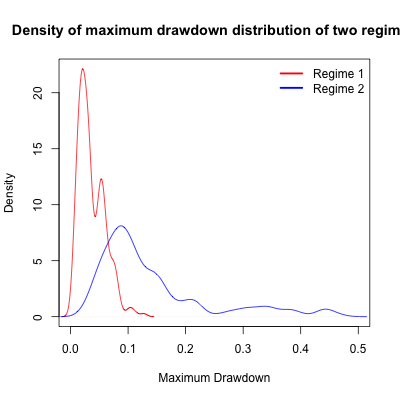
\includegraphics[width=0.7\textwidth]{../results/regime/RMZ_mon1_mdd}
\label{fig: RMZregime_mdd}
\end{figure}

\subsubsection{Rolling risk diagnostics}

For the two regimes in the above section, we calculated the VaR, ES, VaR and maximum drawdown based on one-month rolling window. Based on the rolling risk diagnotics, we are able to calculate and compare the corelation between different risk diagnotics and their difference under high and low volatility regimes. As shown in Table \ref{table:corr_risk_serial_regime}, in high volatility regimes, the correlation between isk diagnostics and serial correlation is higher than in low volatility regimes.

\begin{table}[!h]
\caption{correlation between risk diagnostics and serial correlation of two equal-length episode of each regime} 
\centering 
\begin{tabular}{| r | r | r |} 
 \hline
& Regime 1 & Regime 2 \\
& High volatility & Low volatility \\
 \hline 
corr(VaR, $\rho(1)$)  & -0.29 & 0.08 \\
corr(ES, $\rho(1)$)   & -0.30 & 0.07 \\
corr(volatility, $\rho(1)$)  & -0.33 & 8.4 \\
corr(maximum drawdown, $\rho(1)$)  & -0.24 & 0.07 \\
 \hline
\end{tabular}
\label{table:corr_risk_serial_regime}
\end{table}

\iffalse
\end{document}
\fi

\clearpage

%%%%%%%%%%%%%%%%%%%%%
\section{Time Series -- ARMA model}%%%%
%%%%%%%%%%%%%%%%%%%%%

\iffalse

%-*- program: xelatex -*-        
%-*- program: biber -*-`        
%-*- program: xelatex -*-
\documentclass[12pt]{article}
\usepackage{amsmath,textcomp,amssymb,geometry,graphicx,enumerate,upquote,color}
\usepackage{hyperref}
\usepackage{float}
\usepackage{tikz}
\usepackage{array}
\usepackage{amsfonts}
\def\Session{Fall 2015}
\usepackage[english]{babel}
\title{Relationship between Serial Correlation and Different Risk Measurement}
\author{Boying Gong, Xinyue Zhou}
\newenvironment{qparts}{\begin{enumerate}[{(}a{)}]}{\end{enumerate}}
\def\endproofmark{$\Box$}
\newenvironment{proof}{\par{\bf Proof}:}{\endproofmark\smallskip}
\begin{document}
\maketitle

\fi

\subsection{Explortary Step}
In this section, we have tried to explore the relationship between serial correlation with VaR, ES and CED using several simple time series model. They are AR(1), MA(1) and ARMA(1,1). The three models here are not necessary the best one, or even the ones that all underlying assumptions are satisfied. This step is just try to have a general idea if the serial correlation of each model is related with risk measurements in some way. When it comes to serial correlation here, it refers to the first order autocorrelation of the time series models. 

\subsubsection{AR(1)}

\begin{equation}
X_t = \phi X_{t-1} + \epsilon_t
\end{equation}

AR(1) is the time series model utilized in the paper ON A CONVEX MEASURE OF DRAWDOWN RISK for exploring the relationship between serial correlation and CED of US Equity and US Government Bonds. Here we were trying to implement the same method but expand it to more assets (the eleven US equities). Moreover, we added scatter plots between $\kappa$ and other risk measurements, which enable us to check if CED is more correlated with serial correlation of returns.

Figure \ref{fig:SerCol-VaR5yrAR1}, Figure \ref{fig:SerCol-ES5yrAR1} and Figure \ref{fig:SerCol-CED5yr3monAR1} show the relationship between the theoretical first-order serial correlation and VaR, ES, CED, separately. We can see that the correlation between first-order serial correlation and various risk measures are not so obvious. There are both positive (such as RMZ, BCOM, RAY, USGG10YR) and negative correlations (such as HYG, TIP). The correlation between first-order serial correlation ($\kappa(1)$) and various risk measures are listed in Table \ref{table:corSerialRisk}. We can see from the results that assets such as AGG (0.92) and RMZ (0.90) show high positive correlations, while HYG and TIP show signifiant negative correlation. Moreover, the correlations between VaR ,ES and $\kappa(1)$ are generally greater than the correlation between VaR and $\kappa(1)$.

The Table \ref{table:corSerialRisk} is got from computing the correlation of $\kappa(1)$ and the risk measurement, VaR, ES and CED, which are calculated from the previous study. We also adjust the them to be in the same time period. The time window used for get risk measurements and $\kappa(1)$ is 5 years, and the rolling window within 5 year for CED is 3 month. Consistent with what was showing in the plot, all the assets except MXEA and MXEF have the high correlation between $\kappa(1)$ and risk measurements. Within each asset, as expected, the correlation with VaR and ES are very closed, as VaR is highly correlated with ES internally. However, compared with VaR and ES, the correlation with CED is relatively smaller, and sometimes the correlations are even with different sign. For example, for MXEF asset, the correlation with VaR and ES are positive, and though small, the correlation with CED is negative.

\begin{table}[!h]
\caption{Correlation between $\kappa(1)$ (calculated using AR(1)) and risk measures}
\centering 
\begin{tabular}{ | c || r r r| } 
 \hline
Asset & VaR  & ES & CED \\
  \hline \hline
AGG & 0.92 & 0.95 & 0.94 \\ 
HYG & -0.61 & -0.56 &  -0.41 \\ 
TIP & -0.67 & -0.75 &  -0.73 \\ 
BCOM & 0.86 & 0.80 & 0.76 \\ 
MXEA & 0.26 & 0.33 & 0.08 \\ 
MXEF & 0.23 & 0.22 & -0.05 \\ 
RAY & 0.79 & 0.76 & 0.49 \\ 
RMZ & 0.90 & 0.93 &  0.81 \\ 
SPX & 0.62 & 0.70 & 0.15 \\ 
USGG10YR & 0.67 & 0.64 &  0.66 \\
 \hline
\end{tabular}
\label{table:corSerialRisk}
\end{table}

\iffalse

\begin{figure}
  \caption{First-order serial correlation calculated using AR(1) model versus VaR}
  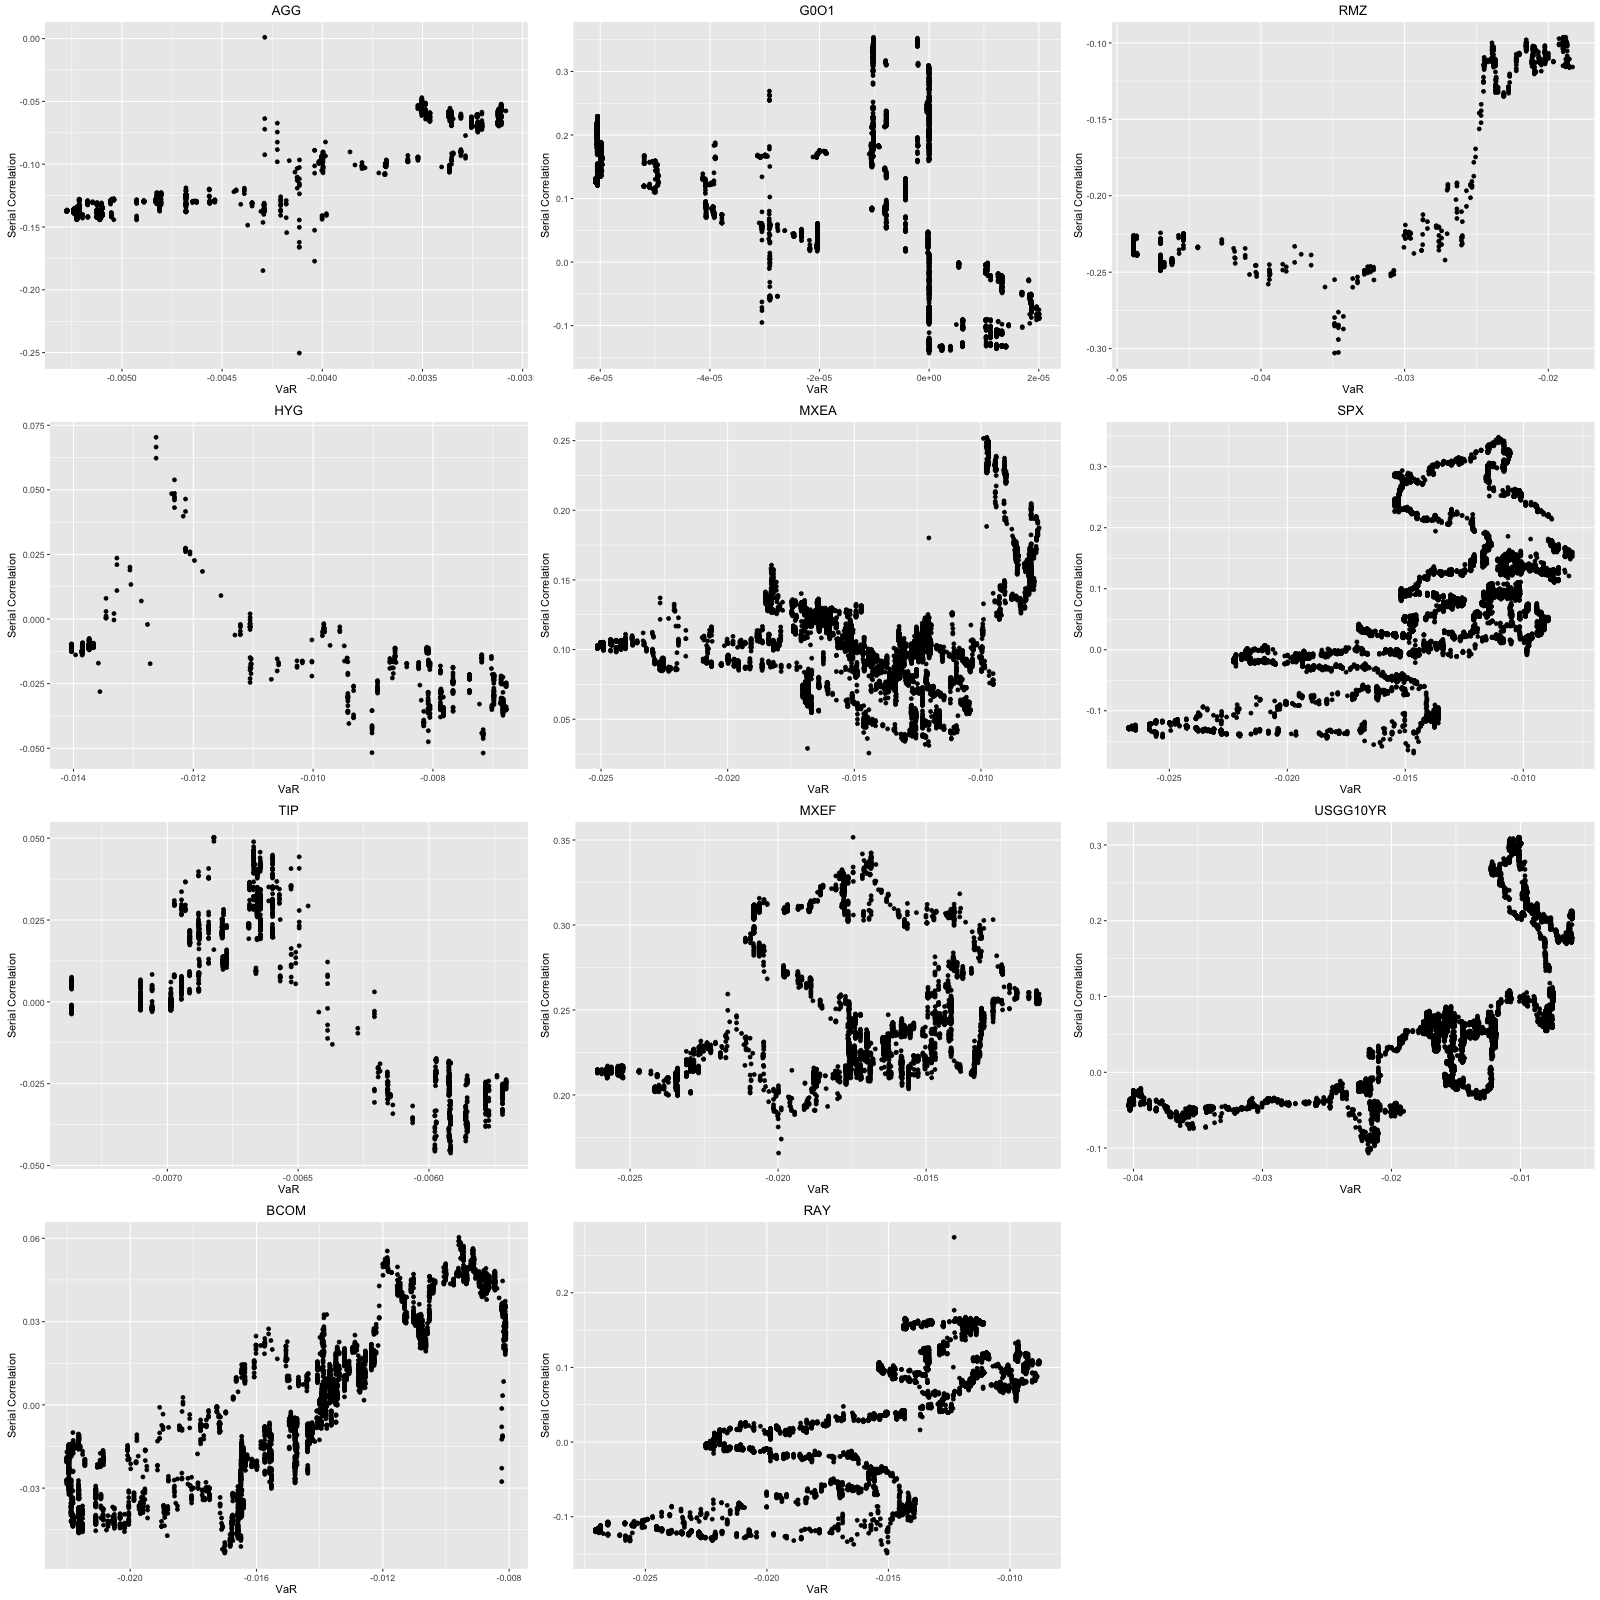
\includegraphics[width = 1\textwidth]{../results/SerCol-VaR5yrAR1}
  \label{fig:SerCol-VaR5yrAR1}
\end{figure}

\begin{figure}
  \caption{First-order serial correlation calculated using AR(1) model versus ES}
  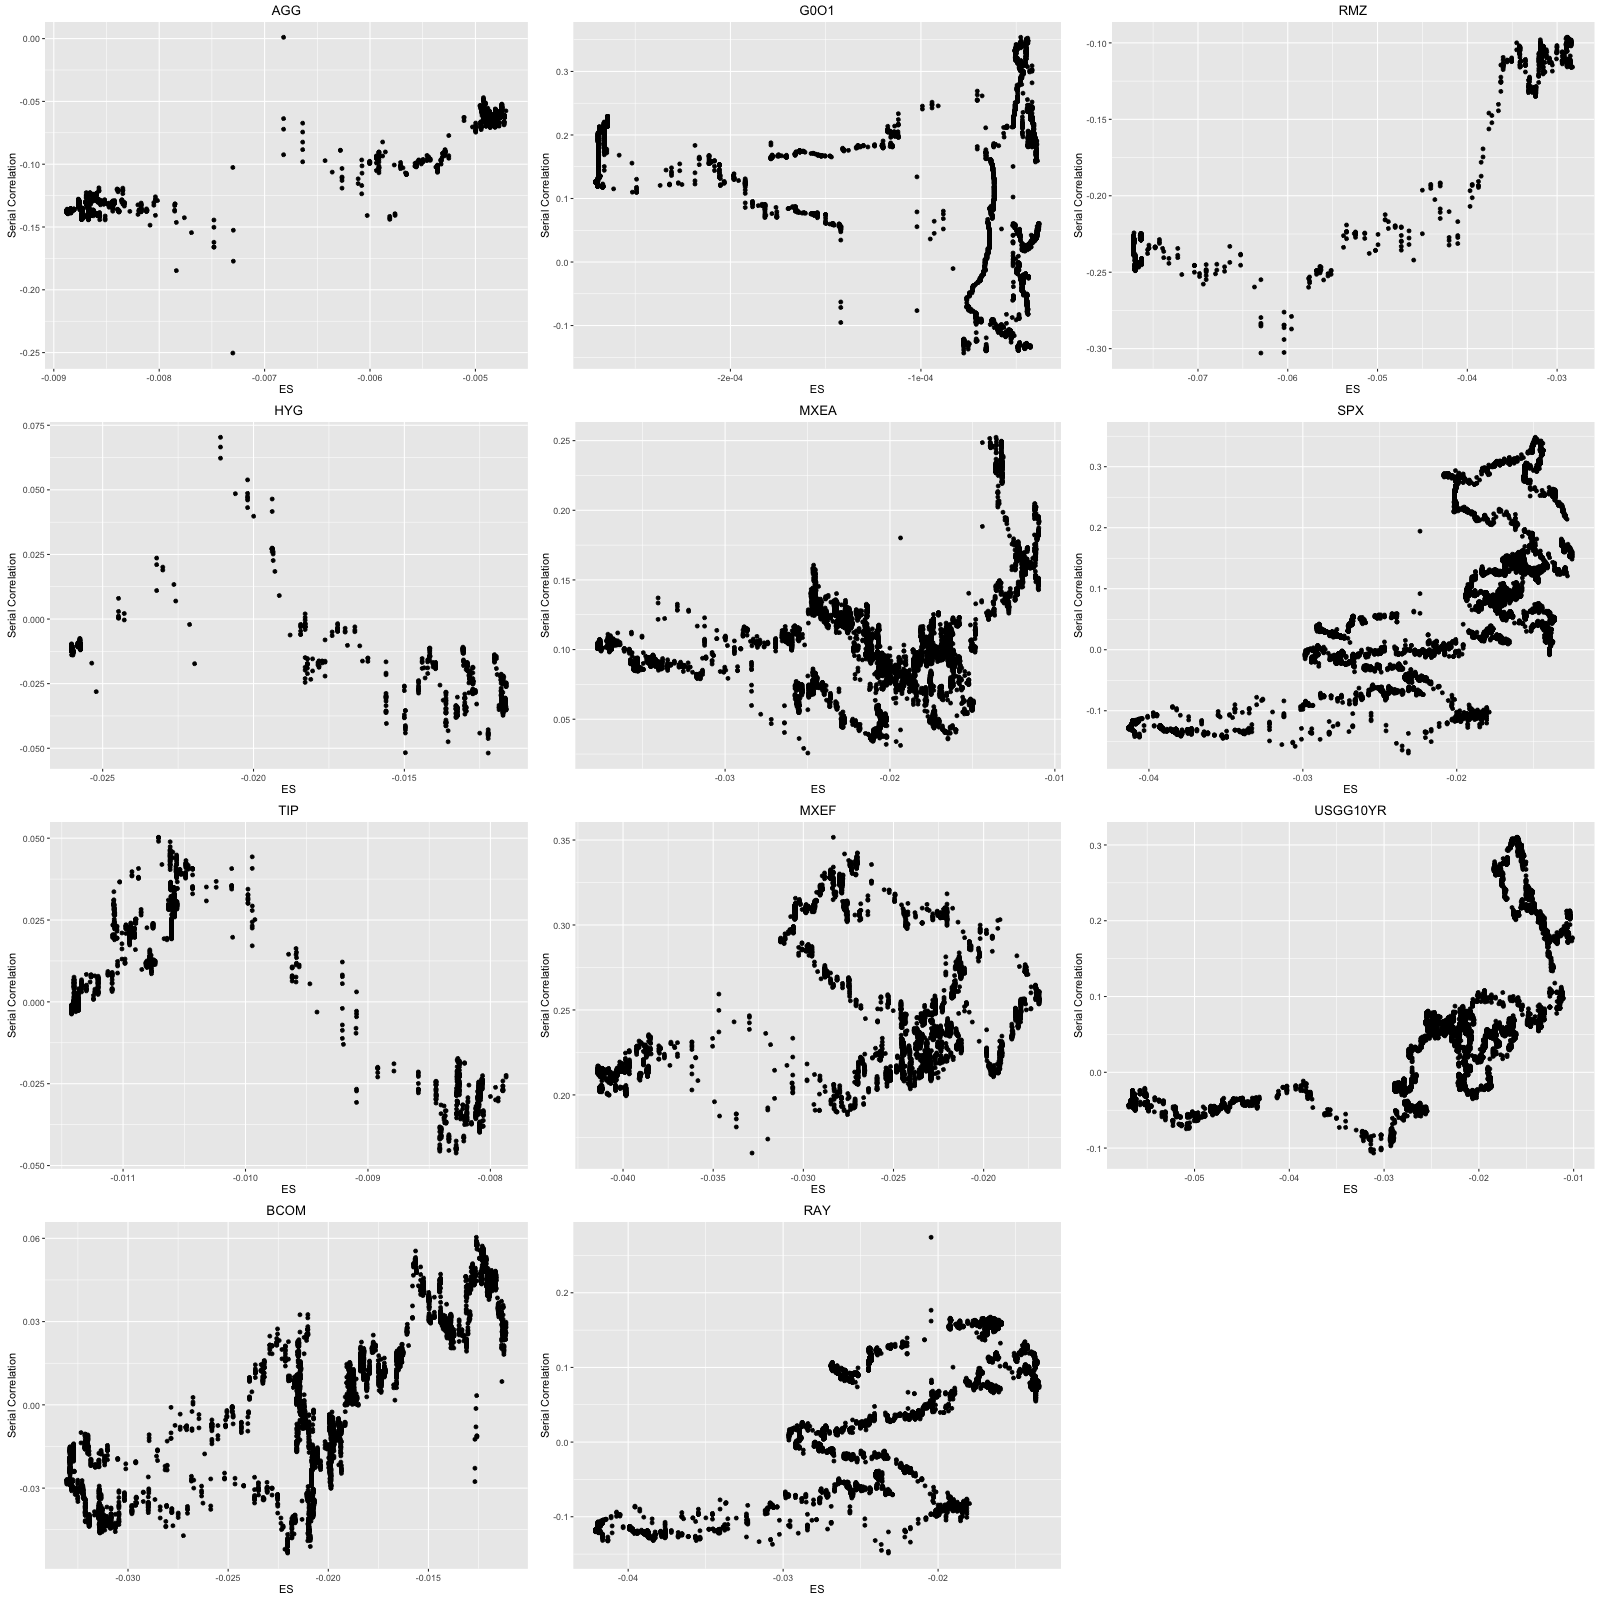
\includegraphics[width = 1\textwidth]{../results/SerCol-ES5yrAR1}
  \label{fig:SerCol-ES5yrAR1}
\end{figure}

\begin{figure}
  \caption{First-order serial correlation calculated using AR(1) model versus CED}
  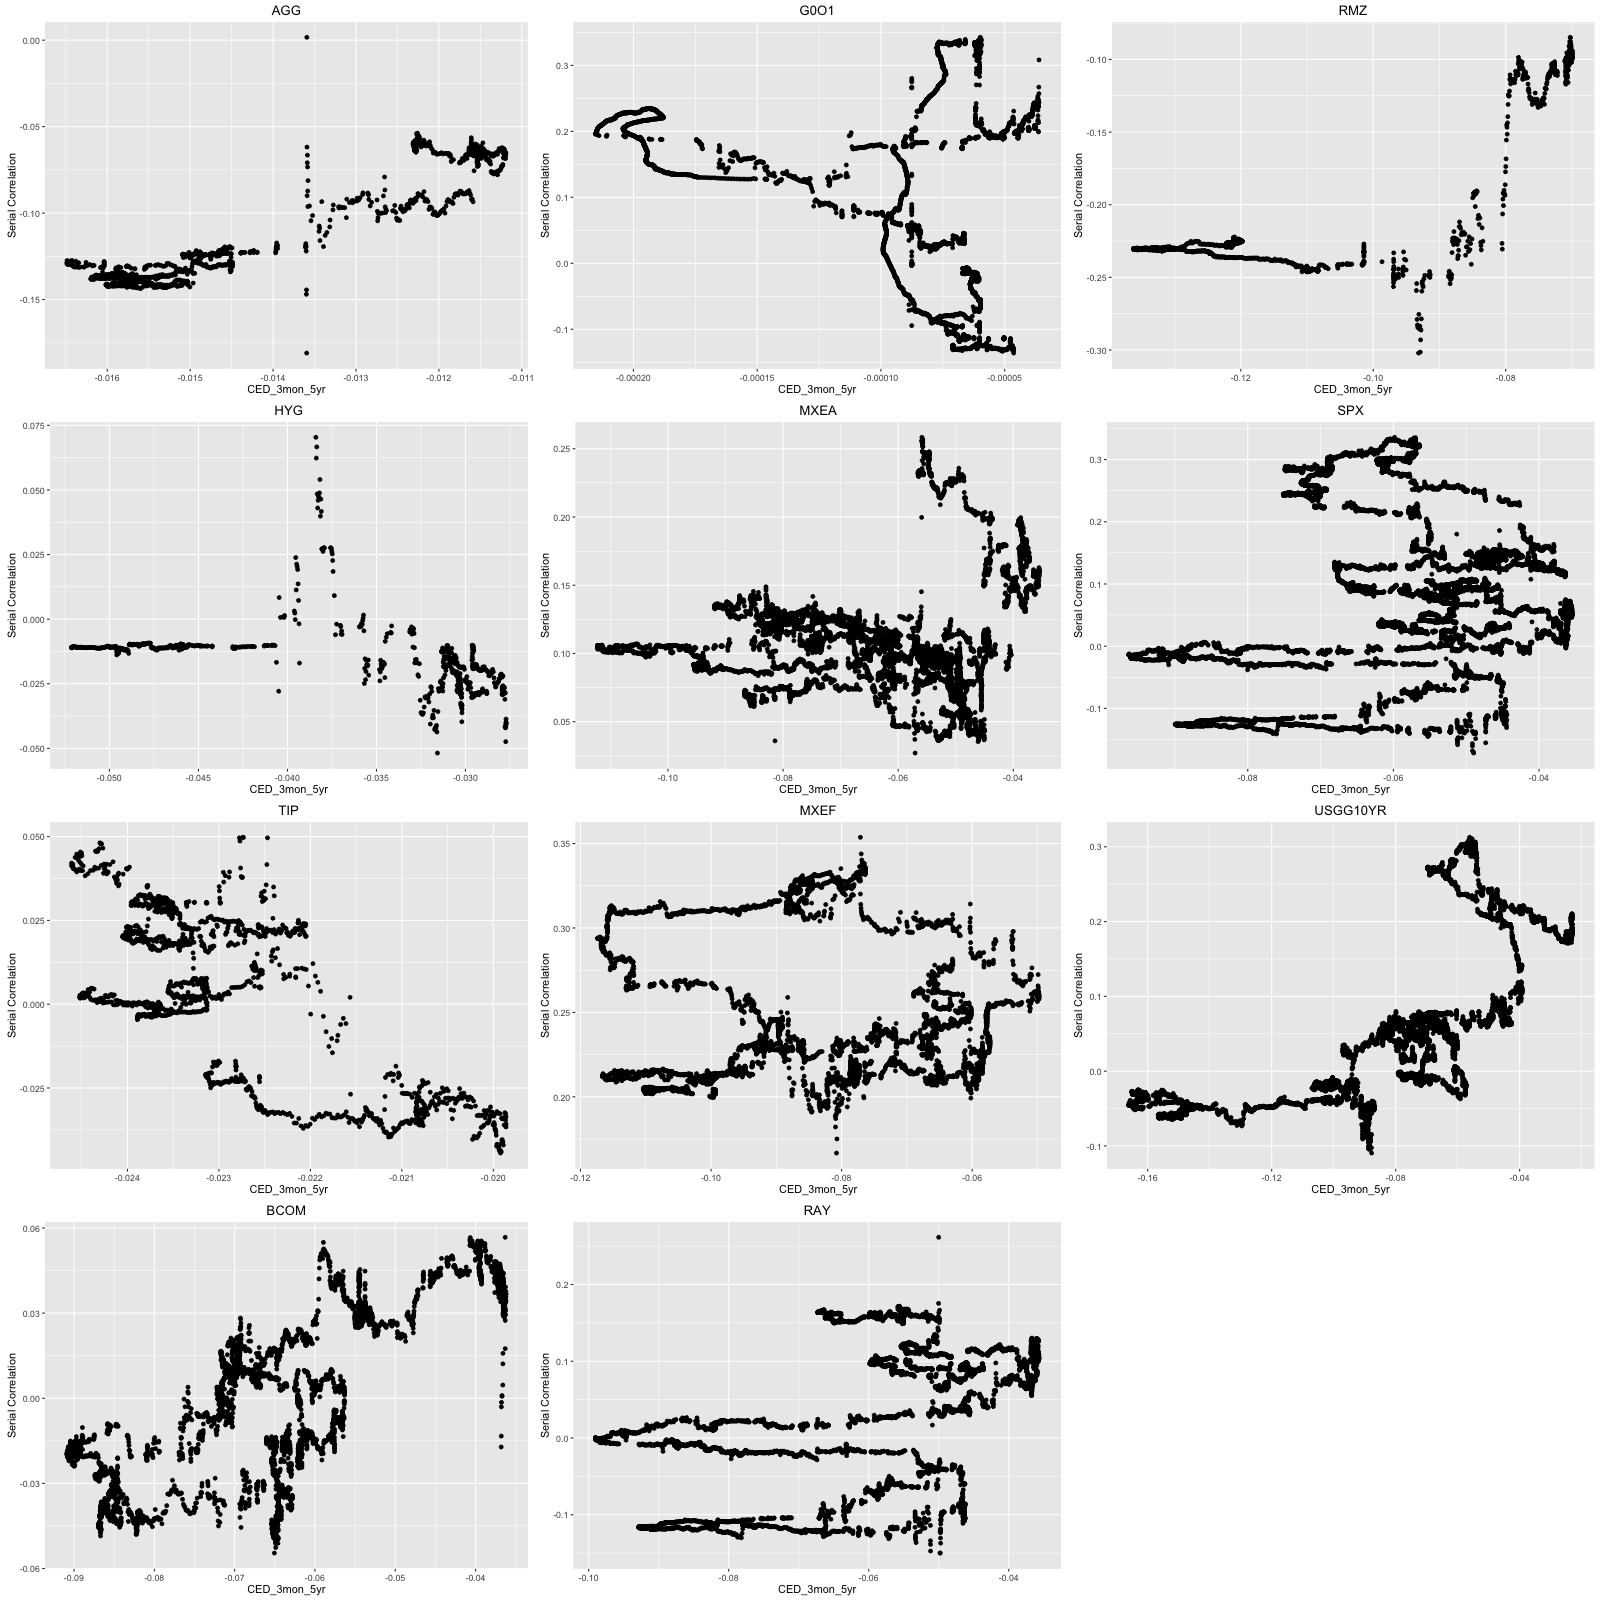
\includegraphics[width = 1\textwidth]{../results/SerCol-CED5yr3monAR1}
  \label{fig:SerCol-CED5yr3monAR1}
\end{figure}

\fi


\subsubsection{MA(1)}
MA(1) is another simple model that is widely used on the Financial time series. In fact, it is a very good one for fitting index \textbf{RMZ}, which will be further elaborated in next section. Since the plot of $\kappa$ vs ES is similar to that with VaR, so only one plot is chosen to put on the report.
\begin{equation}
X_t = \epsilon_t + \theta\epsilon_{t-1}
\end{equation}
For MA(1), there is a simple formula for calculating theoretical first-order serial correlation.
\begin{equation}
\kappa(h) = \begin{cases} \frac{\theta}{(1+\theta^2)} &\mbox{if } h = 1 \\ 
0 & \mbox{otherwise } \end{cases}
\end{equation}

The plots are very similar with that of AR(1) 

\iffalse

\begin{figure}
  \caption{First-order serial correlation calculated using MA(1) model versus VaR}
  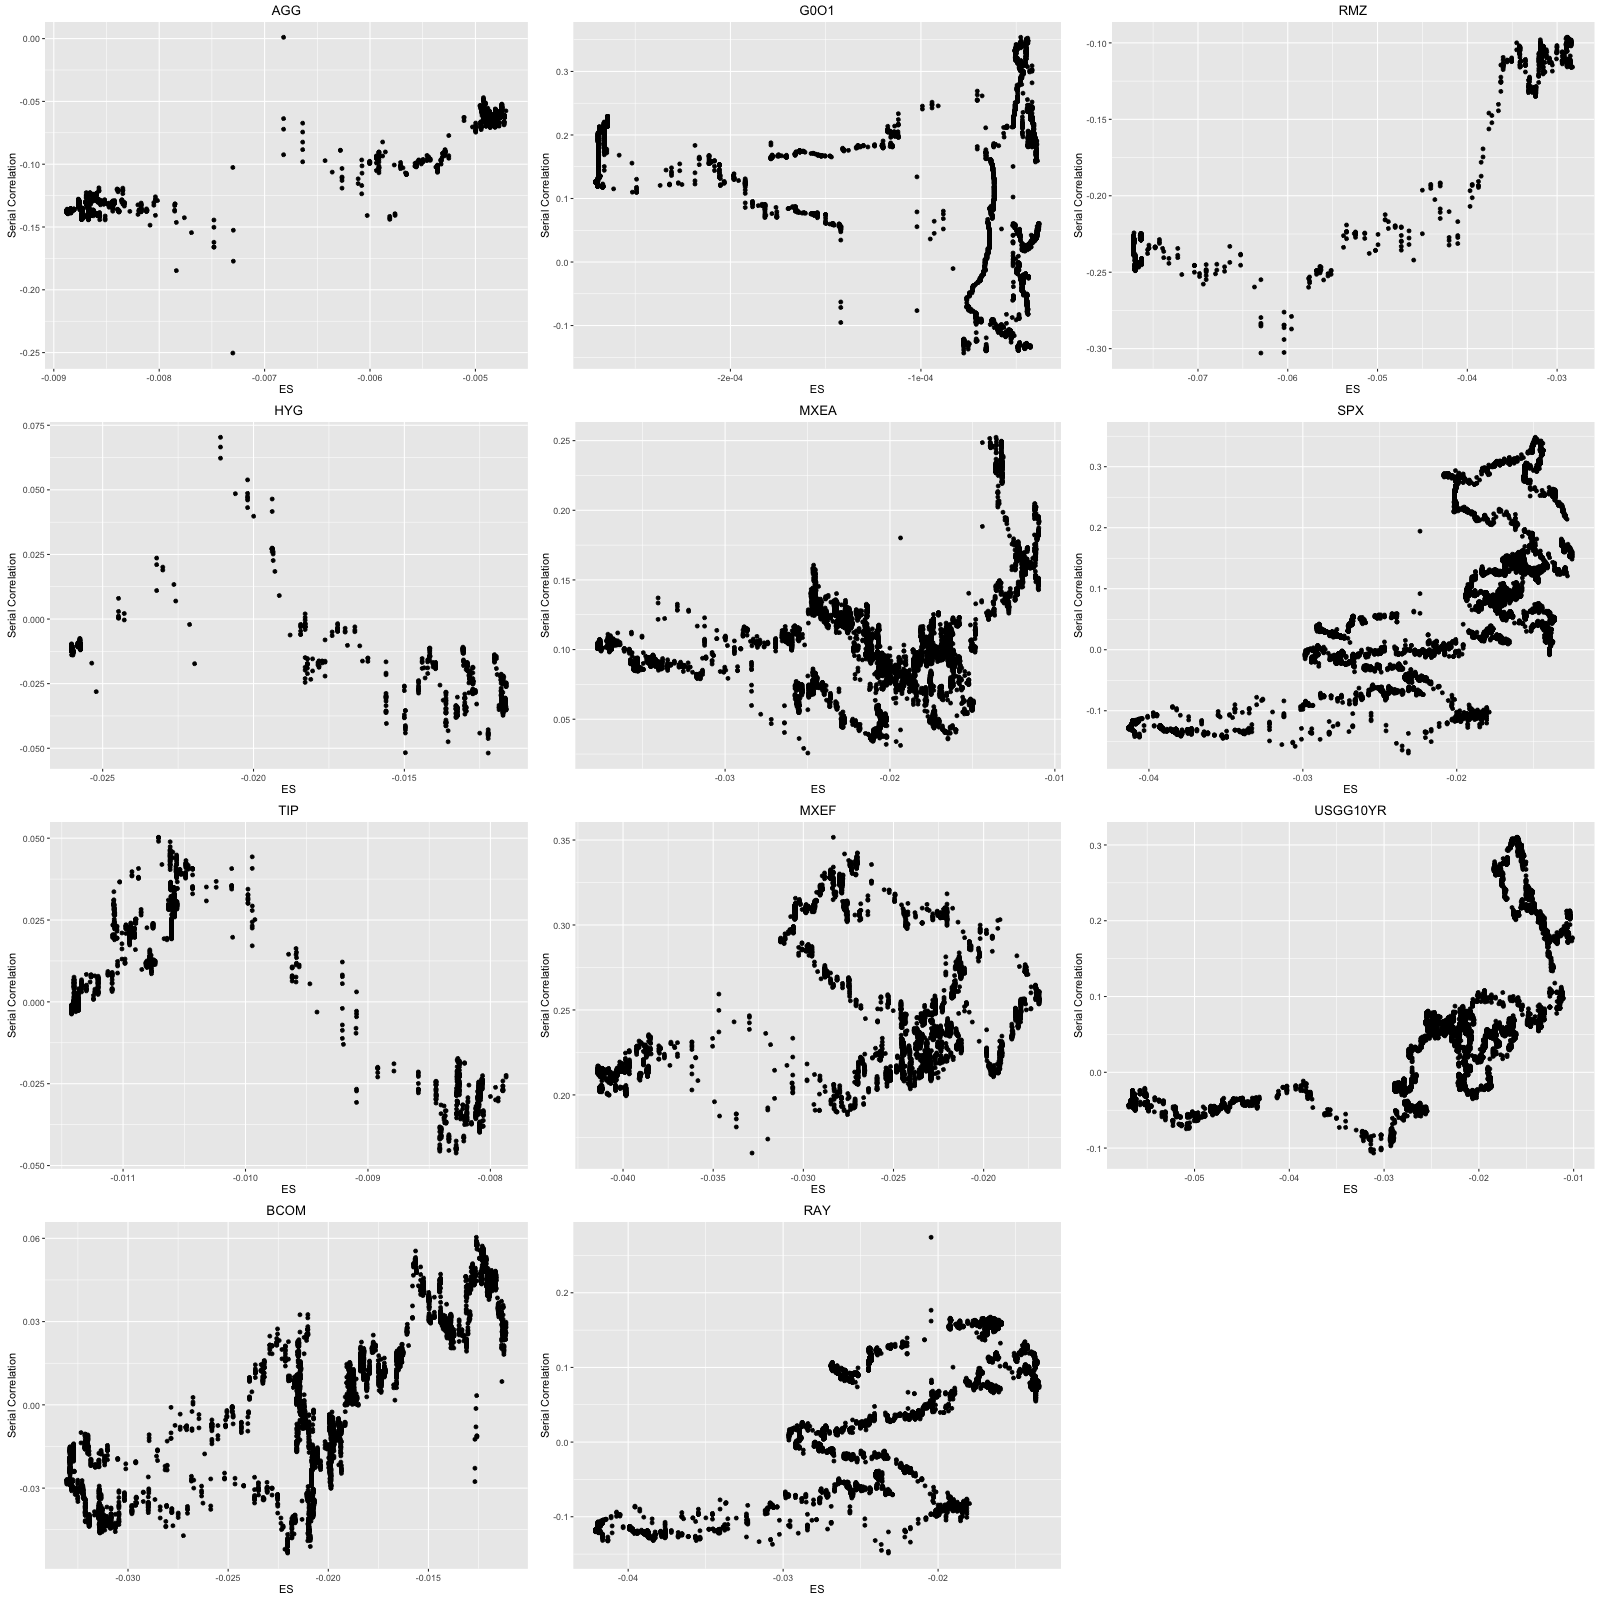
\includegraphics[width = 1\textwidth]{../results/SerCol-ES5yrMA1}
  \label{fig:SerCol-ES5yrMA1}
\end{figure}

\begin{figure}
  \caption{First-order serial correlation calculated using MA(1) model versus CED}
  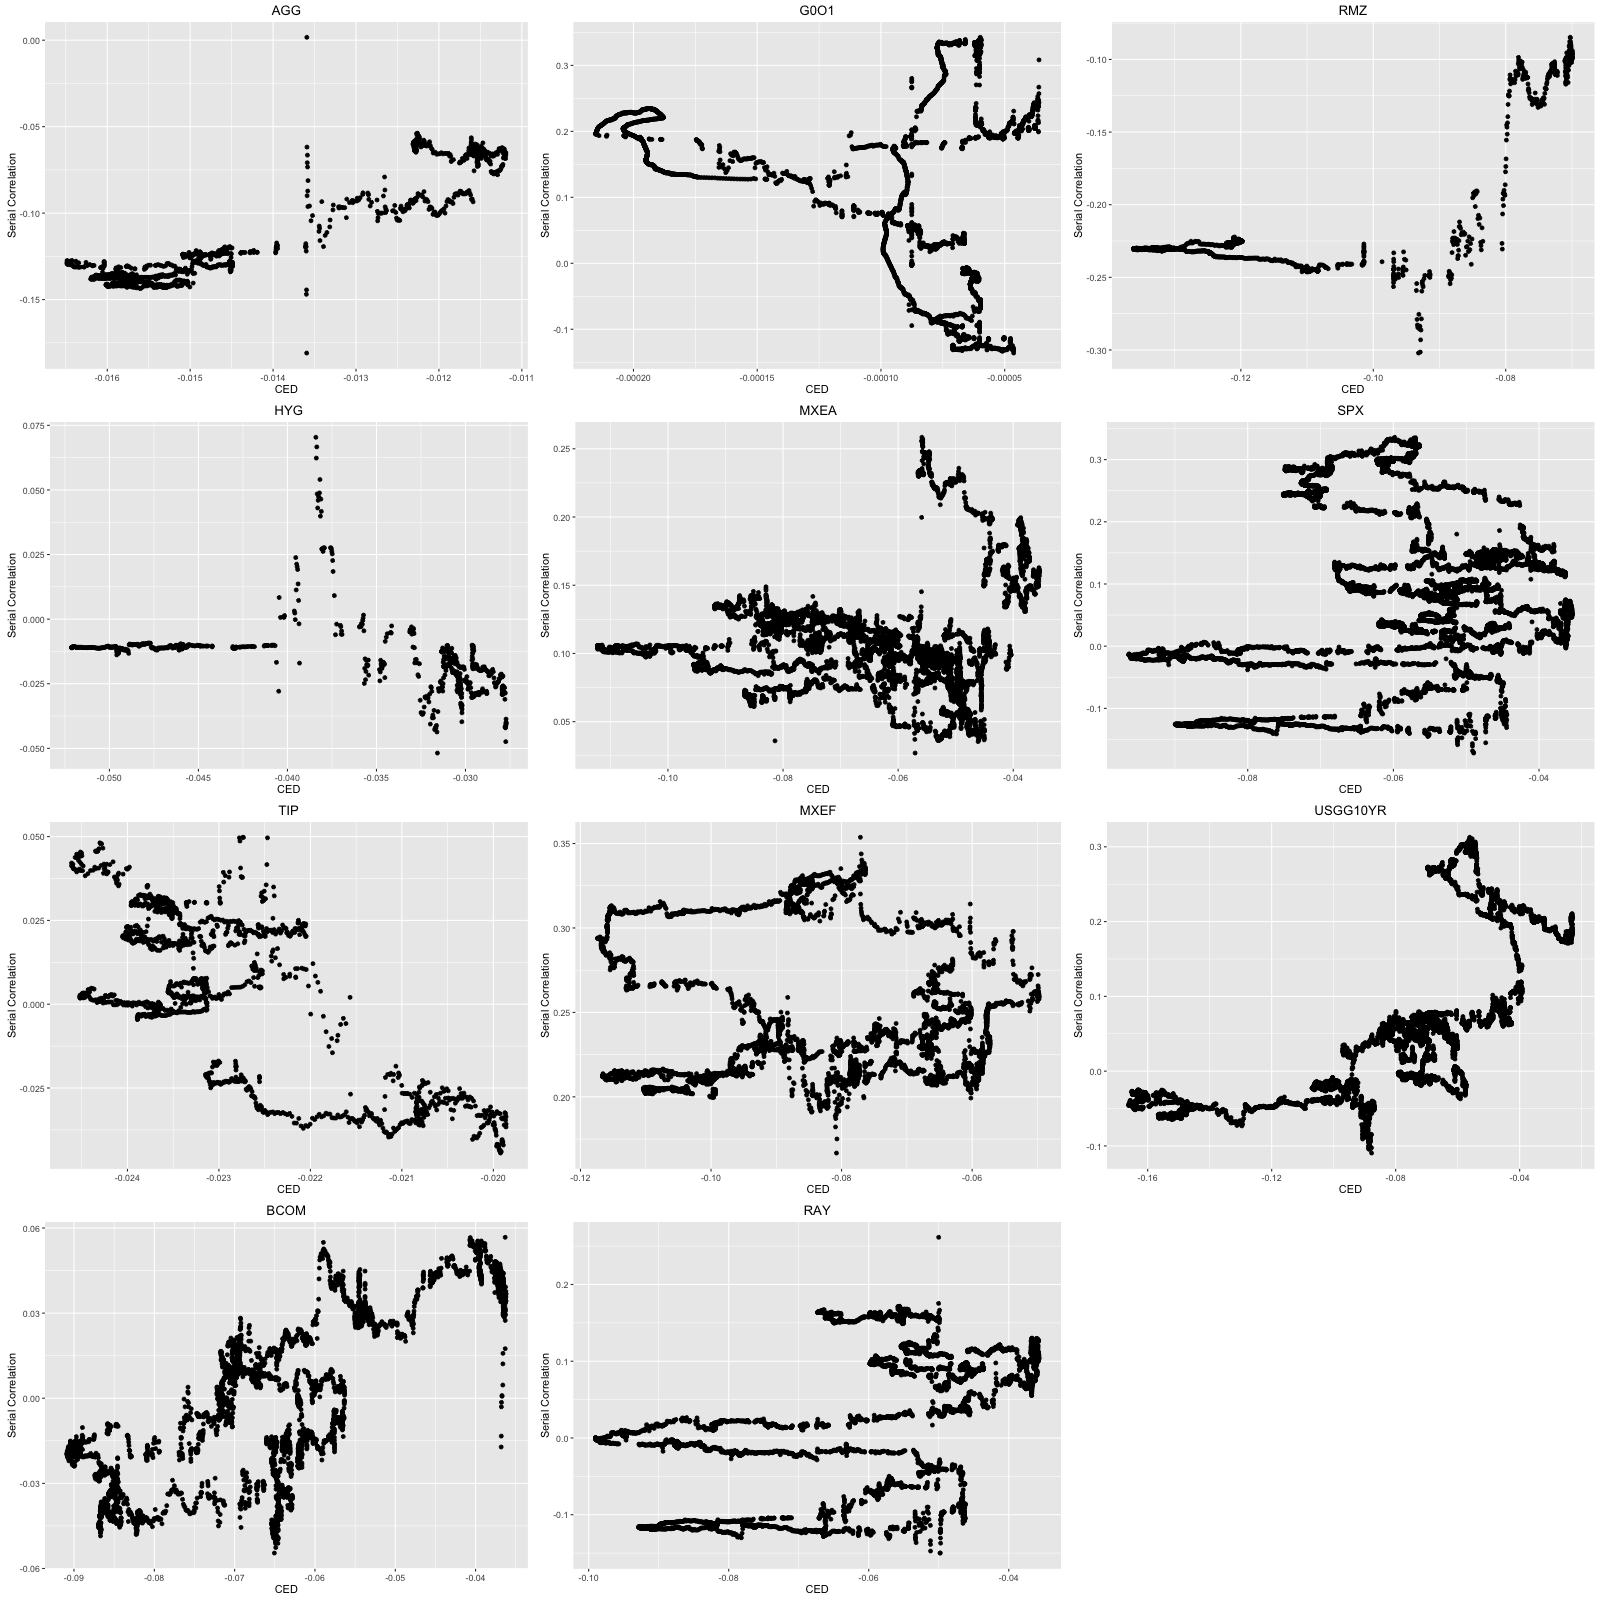
\includegraphics[width = 1\textwidth]{../results/SerCol-CED5yr3monMA1}
  \label{fig:SerCol-CED5yr3monMA1}
\end{figure}

\fi

\begin{table}[!h]
\caption{Correlation between $\kappa(1)$ (calculated using MA(1)) and risk measures}
\centering 
\begin{tabular}{ | c || r r r| } 
 \hline
Asset & VaR  & ES & CED \\
  \hline \hline
AGG & 0.94 & 0.96 & 0.94 \\ 
HYG & -0.51 & -0.45 &  -0.29 \\ 
TIP & -0.65 & -0.74 &  -0.73 \\ 
BCOM & 0.86 & 0.80 & 0.76 \\ 
MXEA & 0.01 & 0.11 & 0.15 \\ 
MXEF & 0.15 & 0.16 & -0.12 \\ 
RAY & 0.79 & 0.77 & 0.50 \\ 
RMZ & 0.92 & 0.95 &  0.84 \\ 
SPX & 0.65 & 0.72 & 0.17 \\ 
USGG10YR & 0.65 & 0.64 &  0.68 \\
 \hline
\end{tabular}
\label{table:corSerialRisk2}
\end{table}

\subsubsection{ARMA(1,1)}

The ARMA(1, 1) has the following expression:

\begin{equation}
X_t = \phi X_{t-1} + \epsilon_t + \theta\epsilon_{t-1}
\end{equation}

The serial correlation calculated using the theoretical expression of fitted ARMA model has a more vague correlation with the various risk measures. The convergence problem occured when fitting the model also indicate a potential model specification.

There is also a formula for calculating the first order correlation for ARMA(1,1) model.
\begin{equation}
\kappa(h) = \frac{(1+\theta \phi)(\theta + \phi)}{1+ 2\theta \phi +\phi^2} \phi^{h-1}, \mbox{if } h \geq 1
\end{equation}

Figure \ref{fig:SerCol-CED5yr3monARMA1} shows the scatter plot of first-order serial correlation calculated using ARMA(1) model versus CED.

\iffalse

\begin{figure}
  \caption{First-order serial correlation calculated using ARMA(1) model versus CED}
  
\includegraphics[width = 1\textwidth]{../results/SerCol-CED5yr3monARMA11}
  \label{fig:SerCol-CED5yr3monARMA1}
\end{figure}

\fi

\subsection{Model Selection}
Things are becoming tricky when it comes to the model selection part. For the fact that it makes no sense to fit different model for each rolling time period within one asset, we tried to find a proper time series model for the all data for each asset. Unfortunately, observing from the ACF plot of returns, they are not stationary by nature without drift term, which means ARMA model is not a good selection for fitting them. It may also explain the reason why the previous section did not produce a expected result that CED is more correlated with serial correlation $\kappa(1)$.

Our criterion here for "better model" is the smaller AIC value. To confirm the fact that ARMA is not reasonable for almost all the indices, we tried sets of parameter for ARMA and select the one with the smallest AIC value. Basically, we chose the combination of AR and MA parameters ranging from 1 to 5.  Here is the results.

AIC short for Akaike information criterion, which is one of the most commonly used criterion for model selection. Here is the formula for AIC.
\[
AIC = 2k - ln(L)
\]
k is the number of parameter in the model and L is the maximum value of the likelihood function for a certain model. Intuitively, AIC rewards goodness of fit (as assessed by the likelihood function), but it also includes a penalty that is an increasing function of the number of estimated parameters \footnote{https://en.wikipedia.org/wiki/Akaike\_information\_criterion}. Therefore, we want the model with smallest AIC value.

\begin{table}[!h]
\caption{Best ARMA Model Based on AIC Value}
\centering 
\begin{tabular}{ | c || r | } 
 \hline
Asset & ARMA (p,q) \\
  \hline \hline
AGG & (5,5)\\ 
HYG & (5,5) \\ 
TIP & (5,4)  \\ 
BCOM & (4,4) \\ 
MXEA & (5,5)  \\ 
MXEF & (5,4) \\ 
RAY & (4,5)  \\ 
RMZ & (3,3)  \\ 
SPX & (5,4) \\ 
USGG10YR & (5,5) \\
 \hline
\end{tabular}
\label{table:bestArmaModel}
\end{table}

From the Table \ref{table:bestArmaModel} almost all the assets, the parameters are as high as 4 or 5, which indicates the time series are not stationary. It also involved some converging issue is when the parameters are getting larger.

For the next step of exploring reasonable model for those assets, several potential models is there can be taken in to consideration:
\begin{itemize}
\item \textbf{ARIMA model with $d=1$}. We found the time series became much more stationary after first-order differencing. 
\item \textbf{ARCH/GARCH model}. Those are the models widely used for financial assets, in which variance of time series are more likely clustering.
\end{itemize}

\subsubsection{EXAMPLE: RMZ data}
Let us take RMZ for example. There are several reasons why we chose to use RMZ: 1) the RMZ has a shorter period, which means a smaller data set to test different time series models. 2) Larger serial correlation and ES, VaR comparing with other indices, implying it is more suitable for analysing the relationship between serial correlation and various risk measures. 3) There are less modes in Maximum drawdown of RMZ, indicating it is reasonable to get tail mean, which is CED.

We also compared RMZ with other index in models selection. From the ACF/PACF plots, RMZ seems the one most suitable for fit ARMA model. Others are not stationary even after a long lag.

First of all, we checked if the time series was stationary in long term. Here is the ACF/PACF plot of the ten-year data. It turns out to be good for using ARMA(0,0,1), MA(1) or ARMA(1,0,1) model, except several lags are a little bit higher than blue line ($|h|$ = 0.05). We also took the first-order difference of the data. The time series become more stationary then before and ARIMA(0,1,1) seems to be a good model for it.

\begin{figure}
  \caption{ACF/PACF of Return for RMZ}
  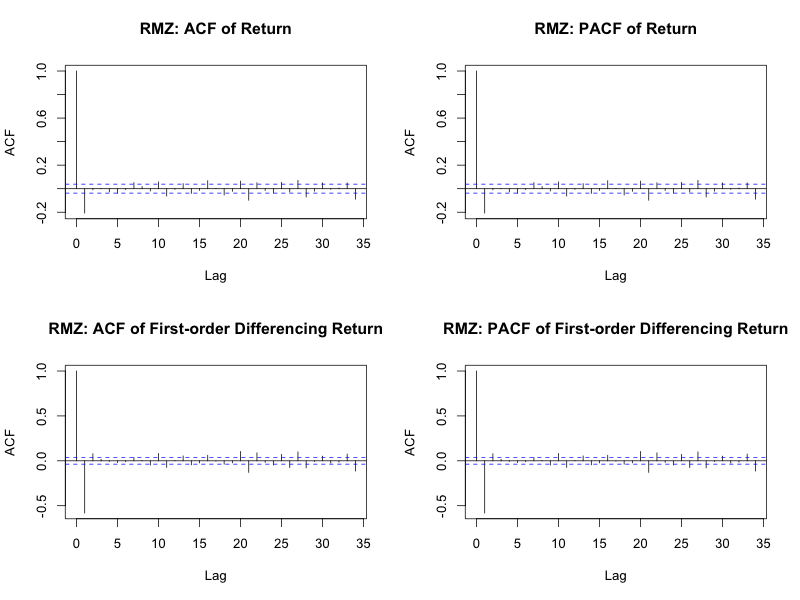
\includegraphics[width = 1\textwidth]{../results/ACFofRMZ}
  \label{fig:ACFofRMZ}
\end{figure}

We also fitted in short time period (1 year period), and the time series became more stationary in each subperiods, and thus the three models mentioned seemed to be reasonable. Below we summarized the model we used for RMZ. We found that the MA(1) model has the smallest AIC within the three parameter sets we chose below. 
\begin{itemize}
\item AR(1) --- to be consistent with your paper
\item MA(1) --- produce least AIC among list 4 models when fitting the all data of RMZ
\item ARMA(1,1)
\item ARIMA(0,1,1) --- Last two is chosen from the pattern of ACF, PACF plot.
\end{itemize}

Here are some diagnostics for MA(1):
\begin{figure}
  \caption{Diagnostic Plots of MA(1) for RMZ}
  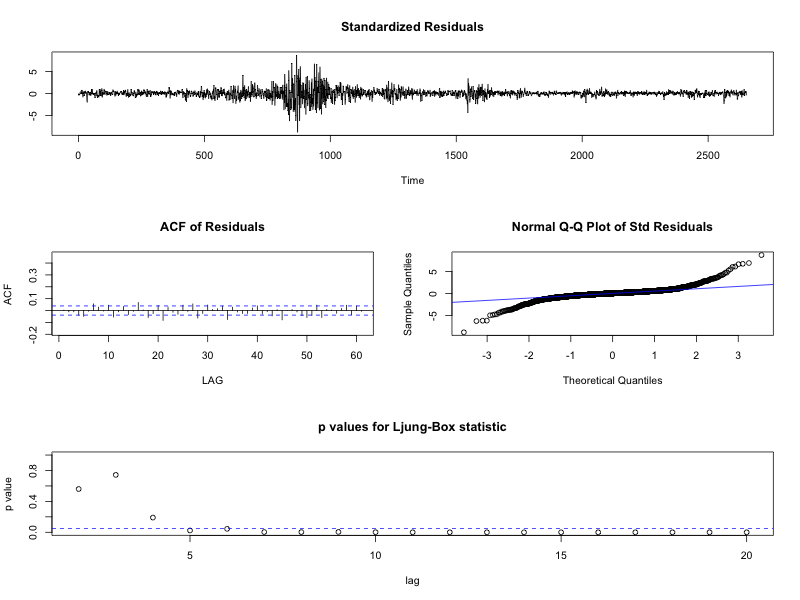
\includegraphics[width = 1\textwidth]{../results/DiagnosticRMZ}
  \label{fig:DiagnosticRMZ}
\end{figure}

From the Figure: \ref{fig:DiagnosticRMZ} above, it is not surprising to see that MA(1) cannot capture the variance cluster in the return, resulting in some variance cluster left the residual plot. There still exists some correlation between residuals after more than 50 lags, but they are comparatively small after the fitting. Normal Q-Q shows that residuals are heavy-tailed. Ljung–Box–Pierce Q-statistic, used for test grouped $\kappa_e(h)$, rejects $H_0$ after $5^{th}$ lag, which also indicates the residual is not white noise after fitting.

In summary, although MA(1) seems to be the good model we could find in ARMA family, it is not enough to capture all the characters in the RMZ return.

\iffalse

\section{Summary: questions}

\subsection{How to find the serial correlation?}

In the paper ON A CONVEX MEASURE OF DRAWDOWN RISK, you fitted the AR(1) model and using the kappa to measure the serial correlation. Now we fit higher order time series model and obtained more than one value of time series coefficient. It's not that reasonable to plot every coefficient versus the risk diagnostics. One solution we came up with is to plot the risk diagnostics versus the serial correlation instead of the time series coefficients. Then how to find serial correlation? 
There are two ways to calculate the serial correlation:
\begin{enumerate}
\item Calculate directly using the return data. For example, for first order serial correlation, we can use $E[X_t X_{t-1}]$;
\item Calculate using the fitted ARMA model. Since we can get the order and coefficients using the fitted model, we may also use them to calculate the theoretical autocorrelation function based on the time series expressions.
\end{enumerate}

We've calculated the serial correlation using both methods, but which one is more reasonable? If the first one is enough, why are we fitting time series model?

\subsection{The correlation between CED and serial correlation is small}

We are supposed to plot the serial correlation verses various risk measure, eg. ES, CED, VaR.  The assumption would be CED is more sensitive to the change of serial correlation, is that right? (And basically we are looking at first order serial correlaion)

We calculated the correlation between first order serial correlation and various risk diagnostics. Then found out they are not that correlated. (with both negative and positive values, compared with the high correlation between various diagnostics which are usually greater than 0.85) Mover, the correlations between serial correlation and CED are even smaller than the correlations between serial correlation and other risk measure. (See Table \ref{table:corSerialRisk})

\subsection{Time series model selection}
 
First, I am curious about the criterion you chose AR(1) for fitting the model in the paper. Is that a common method which is applied to all assets? For our case, when faced more assets with varied property, which criterion are we suppose to use?(right now we use AIC  for model selection). Moreover, when we select the model based on rolling fitting performance, how to choose the criterion? Can we choose to use average AIC, while we think the assumption of using average AIC is the independence between models, which is highly suspicious.


% \bibliographystyle{unsrt}
% \bibliography{analysis}

\end{document}

\fi

\clearpage

%%%%%%%%%%%%%%%%%%%%%
\section{Time Series -- GARCH model}%%%%
%%%%%%%%%%%%%%%%%%%%%

\iffalse
%-*- program: xelatex -*-        
%-*- program: biber -*-`        
%-*- program: xelatex -*-
\documentclass[12pt]{article}
\usepackage{amsmath,textcomp,amssymb,geometry,graphicx,enumerate,upquote,color}
\usepackage{hyperref}
\usepackage{float}
\usepackage{breqn}
\usepackage{tikz}
\usepackage{array}
\usepackage{amsfonts}
\def\Session{Fall 2015}
\usepackage[english]{babel}
\title{Model Selection for the US Indices}
\author{Boying Gong, Xinyue Zhou}
\newenvironment{qparts}{\begin{enumerate}[{(}a{)}]}{\end{enumerate}}
\def\endproofmark{$\Box$}
\newenvironment{proof}{\par{\bf Proof}:}{\endproofmark\smallskip}
\begin{document}
\maketitle
\fi


\subsection{Introduction}
As described in the previous report, for financial assets, the returns have strong dependent across the time, thus it is reasonable to fit time series to interpret and predict them. In the study before,  the ARIMA model is used for fitting, while the diagnostics are infeasible for most assets. They cannot capture the variance cluster in the return, resulting in some variance cluster left the residual plot. In the example of RMZ  before, we are still able to fit at least one `'not too bad'' ARIMA model. However, for other assets, it almost impossible to fit arima: the autocorrelations are still there even after a long lag, and after we adding order more than p = 5, q = 5, the convergence issue always happens. However, we still attach the best ARIMA for each assets we can find to the end.

In this report, we search to apply another widely used model, GARCH,  to fit the returns, and also catch the variance clusters in the them. It turns out to have a much better performance in capturing the variance, and the diagnostic are also showing a delightful patterns

\subsection{Diagnostics of ARMA}
Under our context, Garch models are mainly used for clustered residual left in ARMA model. Therefore, to ensure that GARCH is in need, normally, one should first plot the residuals and other diagnostics of the existing ARMA model. Then from the diagnostics, conclusion can be made if GARCH is necessary and what are the GARCH parameters.

The follow plot is an example of RMZ assets. In the previous study, we found the best ARIMA model for RMZ is MA(1), the diagnostic plot is attached below. Again, the variance clusters in the residual are not captured in the model.

\begin{figure}
  \caption{Diagnostic Plots of MA(1) for RMZ}
  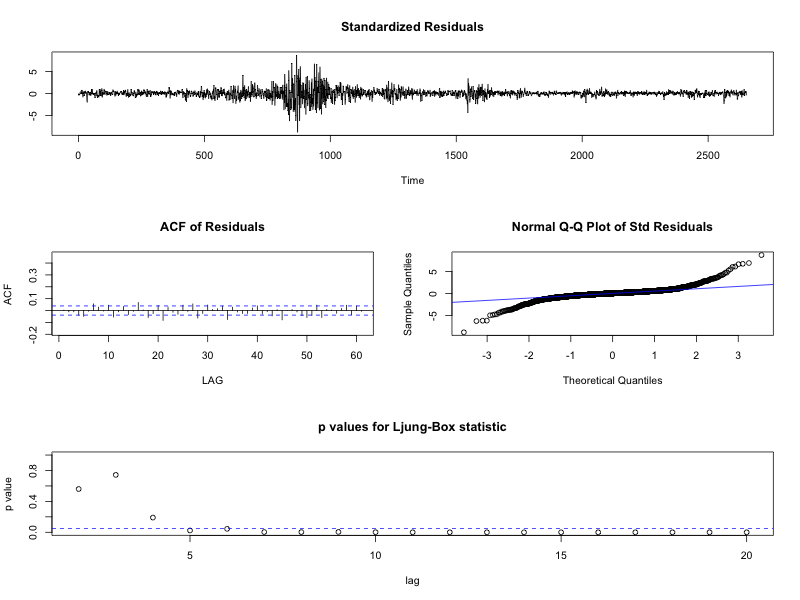
\includegraphics[width = \textwidth]{../results/DiagnosticRMZ}
  \label{fig:DiagnosticRMZ}
\end{figure}

In all the ten American indices, except for \textbf{G0O1}, it is the common phenomenon that assets have the clustered variance, and thus, the GARCH model is in need for model the residuals, as is shown in the Figure \ref{fig:DiagnosticResids}.

\begin{figure}
  \caption{Residuals after fitting using the best ARIMA Model}
  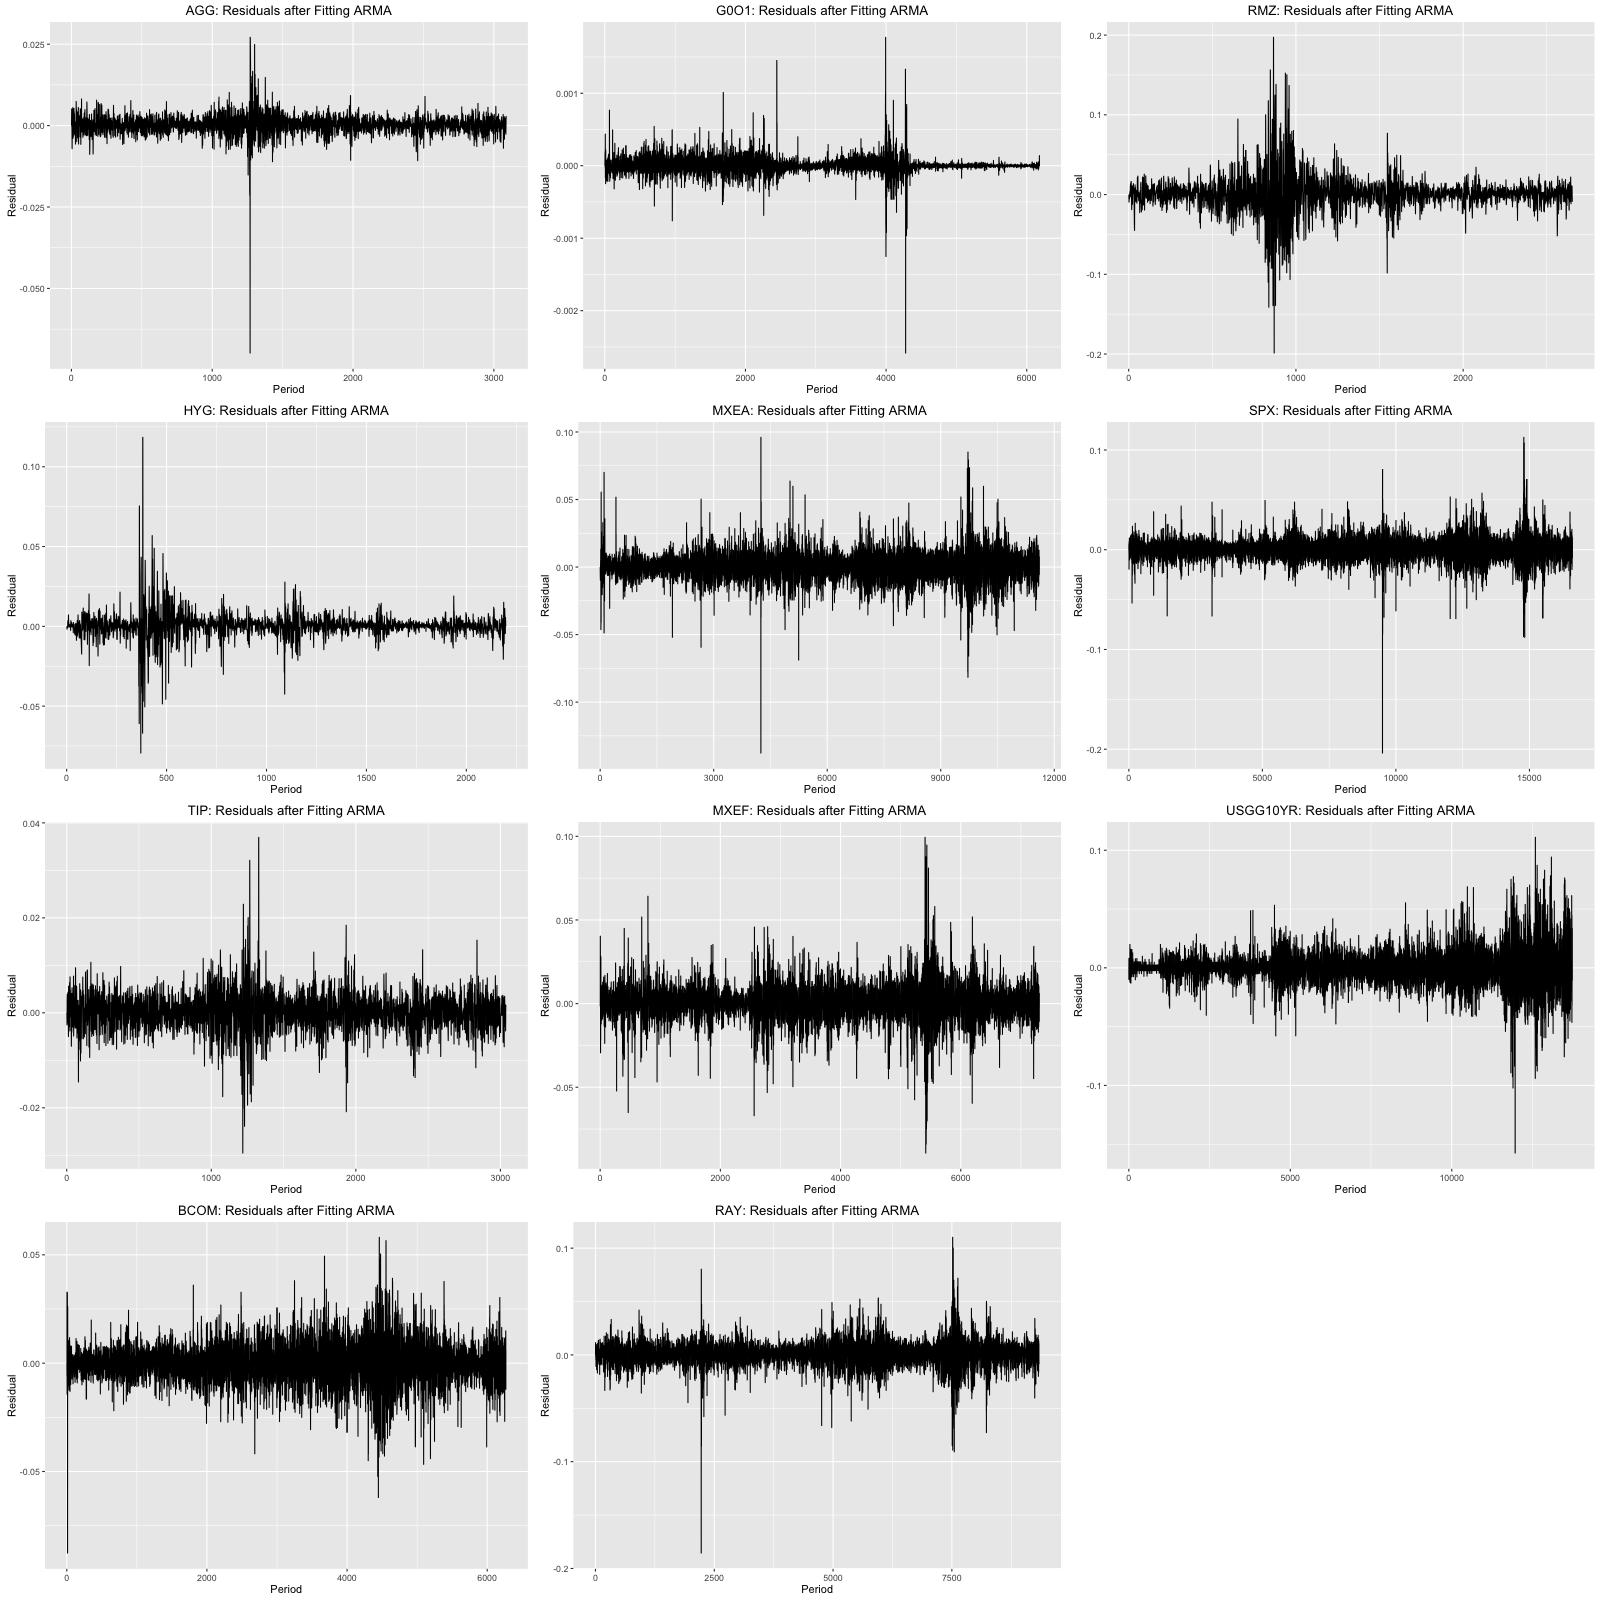
\includegraphics[width = \textwidth]{../results/resids}
  \label{fig:DiagnosticResids}
\end{figure}

The Table \ref{table:BestArima} shows the `'best'' ARIMA model selected from a set of ARIMA parameters. Noticing that model for G0O1is ignored from the analysis, since G0O1 is too stable and always used for free-risk rate.

\begin{table}[!h]
\caption{Best ARIMA Model for the U.S. Assets }
\centering 
\begin{tabular}{ | c || r | } 
 \hline
Asset & ARIMA (p,d,q) \\
  \hline \hline
AGG & (5,0,5) \\ 
HYG & (3,0,1) \\ 
TIP &  (0,0,0)\\ 
BCOM & (0,0,0)\\ 
MXEA & (2,0,2) \\ 
MXEF & (4,0,2)\\ 
RAY &  (2,0,2)\\ 
RMZ & (0,0,1) \\ 
SPX & (2,0,2) \\ 
USGG10YR & (0,0,0) \\
 \hline
\end{tabular}
\label{table:BestArima}
\end{table}

\subsection{Fit Garch Model}
In this section,  RMZ is chosen as an example to explain the process of fitting GARCH, and corresponding diagnostics. RMZ is selected to continue the study in the previous report. RMZ, as shown before, is selected considering its short period, larger series correlaitions, larger risk measurements, and less mode in the Maximum Draw Down.

GARCH(1,1) is the most widely used the model in financial assets, so we fit the residual in MA(1) to GARCH(1,1) here. Rather than ARIMA having constant variance assumption, GARCH(1,1) also model the heteroscedasiticity in the time series.  For GARCH(1,1), the model is discribed as following:

\begin{align*}
y_t & = \sigma_t \epsilon_t\\
\sigma_t^2 & = \alpha_0+ \alpha_1 y_{t-1}^2 +\beta_1\sigma_{t-1}^2
\end{align*}


The residuals left after modeling ARIMA are extracted to feed to GARCH model. The range of GARCH parameters are always hard to figure out just from the plots of diagnostic, so a set GARCH models are applied to each real data. Then we chose the best model based on the BIC criterion. The reason why BIC is used instead of AIC or AICc is that BIC always penalize more on extra parameters and suggest a smaller model, avoiding the overfitting problem.

After fitting the GARCH models on the residuals left from ARMA models, diagnostics are conducted on each GARCH model. It is a common situation that all the autocorrelations between residuals have been highly reduced after modeling, which mean GARCH effectively model the residuals. The Table \ref{table:BestGarch} present the best GARCH model according to BIC values. 

\begin{table}[!h]
\caption{Best GARCH Model for the residuals after Fitting ARIMA}
\centering 
\begin{tabular}{ | c || r | } 
 \hline
Asset & ARIMA (p,q)+ GARCH(m,n) \\
  \hline \hline
AGG & ARMA(5,5)+GARCH(1,1) \\ 
HYG & ARMA(3,1)+GARCH(1,1) \\ 
TIP &  GARCH(1,1)\\ 
BCOM & GARCH(1,1)\\ 
MXEA & ARMA(2,2)+ GARCH(1,2) \\ 
MXEF & ARMA(4,2) + GARCH(1,1)\\ 
RAY &  ARMA(2,2) + GARCH(1,1)\\ 
RMZ & MA(1) + GARCH(1,1) \\ 
SPX & ARMA(2,2) +GARCH(1,1)\\ 
USGG10YR & GARCH(1,3) \\
 \hline
\end{tabular}
\label{table:BestGarch}
\end{table}


 We are also faced with several problems in diagnostics, after finding the most reasonable GARCH parameters. The first thing needs to be mentioned is that it always appears heavy tail problem after fitting.  The residual left after GARCH is almost white noise  , which is a good sign for eliminating the correlations between points, as ACF plots. However, the heavy tail is existing as the sign from the normal Q-Q plots   , in which points deviate from line at both ends. Several approach can be adopted to fix heavy tail, one of which is that instead of normal, using Student t distribution as conditional distribution in the GARCH. Alternatively, Generalize Normal Distribution (GED) can also used as conditional distribution to somehow alleviate heavy tail. QMLE is another potential option. 
 
 The other concern we meet in the analysis is that, even though after fitting GARCH, some of the autocorrelation still left in the residuals, and it more commonly happens on the first order correlation. Several derivative class of GARCH model are specifically used for handle this problem, while we left it for future analysis, as it does no harm for our prime research.


\subsubsection{An Example: RMZ}
In the previous study, we found the best ARIMA model for RMZ is MA(1), the diagnostic plot is attached below. Again, the variance clusters in the residual are not captured in the model.

\begin{figure}
  \caption{Diagnostic Plots of MA(1) for RMZ}
  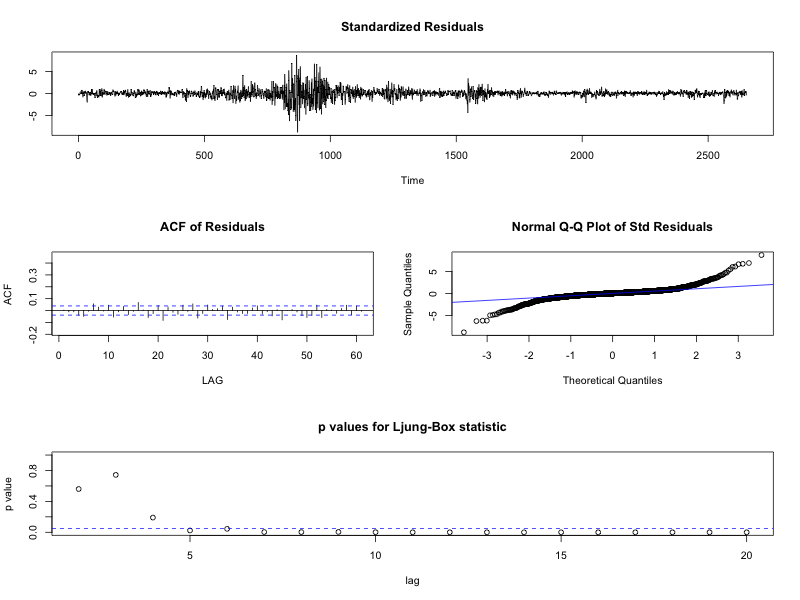
\includegraphics[width = \textwidth]{../results/DiagnosticRMZ}
  \label{fig:DiagnosticRMZ}
\end{figure}

Fit the residual of MA(1) to GARCH(1,1), we got the follow model:
\begin{align*}
R_t &= -4.1561\times 10^{-2}\epsilon_{t-1} \\
\sigma_t^2 & = 1.9955 \times 10^{-6} +1.1083\times 10^{-1} T_{t-1}^2 +8.8506\times 10^{-1}  \sigma_{t-1}^2
\end{align*}

The Figure: \ref{fig:RMZ_GARCH_dig1} are the plots of the standardized residuals. 

\begin{figure}
  \caption{RMZ: Diagnostic Plots of GARCH(1,1) with Gaussian Conditonal Distribution}
  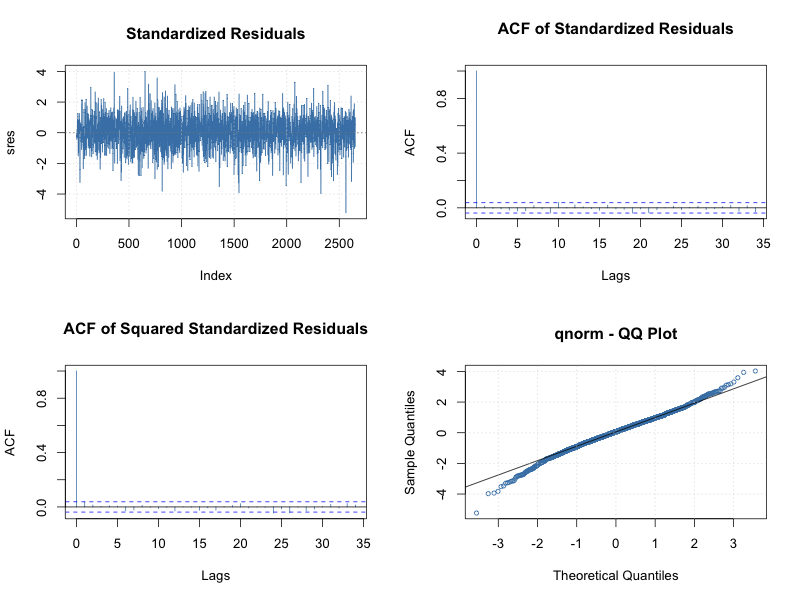
\includegraphics[width = \textwidth]{../results/RMZ_GARCH_dig1}
  \label{fig:RMZ_GARCH_dig1}
\end{figure}

After fitting GARCH, the residual left is almost white noise, which is a good sign for eliminating the correlations between points, as evidented in the next two ACF plots. However, the heavy tail problem is still there. Several approach can be adopted to fix it, one of which is instead of normal, using Student t distribution as conditional distribution in the GARCH. Finding t distribution is not really solve the problem, we finally chose to use Generalize Normal Distribution (GED) as the conditional distribution. QMLE is another potential alternative. The Figure: \ref{fig:RMZ_GARCH_dig2} indicates that the heavy tail problem is almost solved in the by applying GED.

\begin{figure}
  \caption{RMZ: Diagnostic Plots of GARCH(1,1) with GED Conditonal Distribution}
  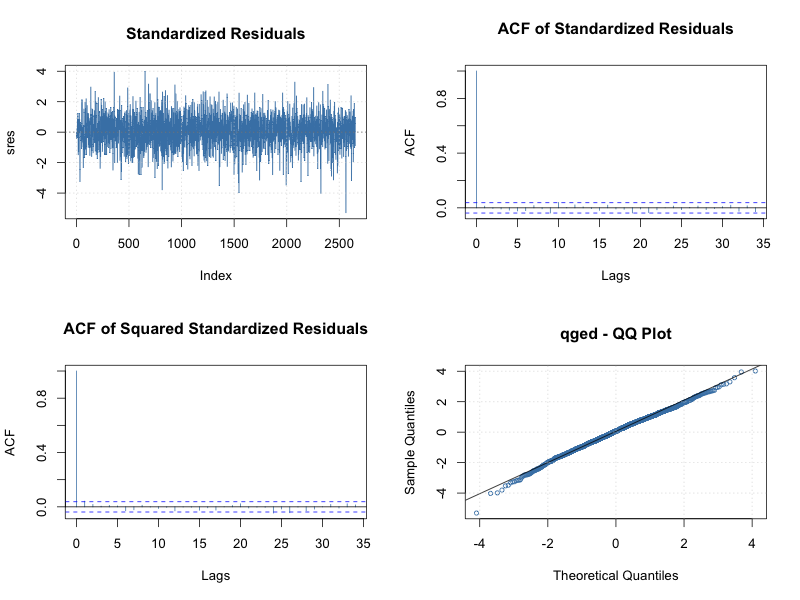
\includegraphics[width = \textwidth]{../results/RMZ_GARCH_dig2}
  \label{fig:RMZ_GARCH_dig2}
\end{figure}

Figure \ref{fig:RMZ_GARCH_ESTsd} the plot compare the estimation of standard deviation using GARCH(1,1), with using naive estimate of standard deviation. The black continuous line is the estimate of the instantaneous conditional standard deviation of the GARCH(1,1). The large peak indicative of the huge standard deviation corresponding to the crisis of 2008. Red line is the empirical standard deviation of the entries of the series in the window containing the entries of the last 30 days.  As shown in the plot, the naive estimator is smoother than GARCH, while they almost follow the sample trend.
\begin{figure}
  \caption{RMZ: Estimate of the Instantaneous Conditional Standard Deviation}
  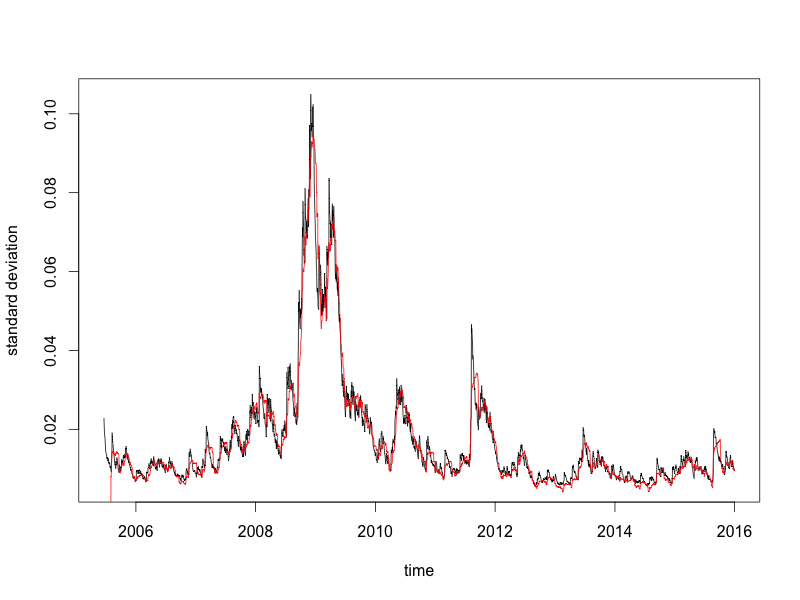
\includegraphics[width = \textwidth]{../results/RMZ_GARCH_ESTsd}
  \label{fig:RMZ_GARCH_ESTsd}
\end{figure}

Figure \ref{fig:RMZ_GARCH_predCI} show the last 120 residuals from MA(1), we used all but last 20 to fit the GARCH(1,1) model with GED conditional distribution and create an confident interval based on that. And it is nice to see that all the last 20 points lies in the interval.

\begin{figure}
  \caption{RMZ: Estimate of the Instantaneous Conditional Standard Deviation}
  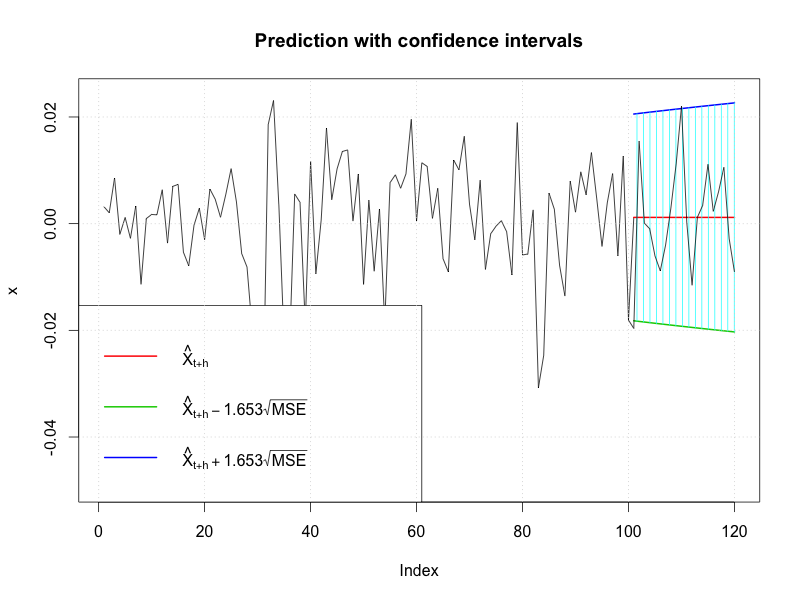
\includegraphics[width = \textwidth]{../results/RMZ_GARCH_predCI}
  \label{fig:RMZ_GARCH_predCI}
\end{figure}

In summary, instead of assuming constant variance using ARIMA, modeling the residuals from MA(1) using GARCH(1,1) seems to be more reasonable for RMZ.

\subsubsection{Summary of Results}
This section answer the questions that what kind of model should be selected for modeling the return of financial assets. Model selection hints from the descriptive statistics are also highlighted. It gives people an intuition and helps to narrow down the potential parameter sets, and thus reduce the work load. However, this is not the general rule. In order to decide the most suitable model, one should take a close look at the time series properties and compare several possible models using model selection criterions.

\begin{itemize}
\item Essentially, ARMA component do not need to be there. For those time series, conditional means are almost fixed, such as TIP, BCOM and USGG10YR. Some of statistics are able to indicate this on some extent. For example, a very high Sharpe Ratio, meaning the low return and high standard deviation, suggests that it is hard for using ARIMA  to capture the change of conditional mean in too much noise. Moreover, based on study, we found that the returns of assets with smaller absolute skewness values are more likely free from ARMA component. As can be imagined, if an asset is high skewed, it is a highly possible situation that the returns deviate from mean value at some certain time period because of economics events.
\item ARMA component sometimes is just not enough to characterize the timeseries, indicated a unstationary residuals even after a long lag. Based on my experience, the trial until p =5 and q = 5 is adequately detection for ARMA component. The change of model or adding GARCH component should be taken into consideration when larger lags in need.
 \item For the financial essets we already took a close look at, the GARCH model is always required, as the evidenced by the clustered variance in the return. Financial assets tend to have higher or lower volatility in a certain period as the result of some economics events, such as a higher fluctuation around 2008 crisis.
  \item GARCH(1,1) are always enough for charaterize the clustered variance in financial assets. Even though I select GARCH(1,2) and GARCH(1,3) for MXEA and USGG10YR based on BIC, GARCH(1,1) still works good for these two indices, showing almost no differents in diagnostic plots. 
\end{itemize}


Next present the model for each index. Those are from analysis that repeat over and over again in the previous section. To avoid redundancy, the full analysis is not showing out. The stars in the equations below represents the significance level of the coefficents. 


\begin{enumerate}
\item \textbf{AGG} (BIC = -6.8688):
\begin{dmath*}
R_t  = -0.0698R_{t-1} + 0.5235R_{t-2} - 0.7308R_{t-3}- 0.4478 R_{t-4}
+0.5656 R_{t-5} -0.0771 \epsilon_{t-1}  -0.5810\epsilon_{t-2} 
+0.774\epsilon_{t-3} +0.3736\times 10^{-4}\epsilon_{t-4}  -0.6190 \epsilon_{t-5} 
\end{dmath*}
\begin{align*}
\sigma_t^2  = 9.3294 \times 10^{-8} +6.8088\times 10^{-2} T_{t-1}^2(^{***}) +9.1898\times 10^{-1}  \sigma_{t-1}^2(^{***})\\
\end{align*}


\item \textbf{HYG} (BIC = -6.8688):
\begin{dmath*}
R_t = -0.5756R_{t-1} -0.0207R_{t-2}  -0.0996R_{t-3}
+ 0.5775 \epsilon_{t-1} 
\end{dmath*}
\begin{align*}
\sigma_t^2  &= 4.312 \times 10^{-7} +1.712\times 10^{-1} T_{t-1}^2(^{***}) +8.467\times 10^{-1}  \sigma_{t-1}^2(^{***})\\
\end{align*}

\item \textbf{TIP} (BIC = -8.3838):
\begin{align*}
\sigma_t^2  &= 1.752 \times 10^{-7} +5.254\times 10^{-2} T_{t-1}^2(^{***}) +9.357e\times 10^{-1}  \sigma_{t-1}^2(^{***})\\
\end{align*}


\item \textbf{BCOM} (BIC =-6.7632):
\begin{align*}
\sigma_t^2  &= 2.640 \times 10^{-7} +4.536\times 10^{-2} T_{t-1}^2(^{***}) +9.523e\times 10^{-1}  \sigma_{t-1}^2(^{***})\\
\end{align*}

\item \textbf{MXEA} (BIC = -6.7857):
\begin{dmath*}
R_t = -0.2176R_{t-1} -0.4230R_{t-2} 
 0.3240\epsilon_{t-1} + 0.4305 \epsilon_{t-2} + 0.0248 \epsilon_{t-3} +  0.0394 \epsilon_{t-4} 
\end{dmath*}
\begin{dmath*}
\sigma_t^2  = 1.1415\times 10^{-6} +1.2141\times 10^{-1} T_{t-1}^2(^{***}) +5.1514\times 10^{-1}  \sigma_{t-1}^2(^{***}) +3.5499\times 10^{-1}  \sigma_{t-2}^2(^{***})\\
\end{dmath*}


\item \textbf{MXEF} (BIC =-6.5399):
\begin{dmath*}
R_t = -0.6328R_{t-1}+  0.1588R_{t-2} -0.0038R_{t-3}  -0.0093R_{t-4} +
 0.8807\epsilon_{t-1} +  0.0279 \epsilon_{t-2} 
\end{dmath*}
\begin{dmath*}
\sigma_t^2  = 1.4479\times 10^{-6} + 9.8248\times 10^{-2} T_{t-1}^2(^{***}) +8.9191\times 10^{-1}  \sigma_{t-1}^2(^{***}) \\
\end{dmath*}


\item \textbf{RAY} (BIC =-6.6313):
\begin{dmath*}
R_t = 0.2526R_{t-1}+  0.3255R_{t-2} -0.2553\epsilon_{t-1} -0.3649 \epsilon_{t-2} 
\end{dmath*}
\begin{dmath*}
\sigma_t^2  = 1.1770\times 10^{-6} + 7.2784\times 10^{-2} T_{t-1}^2(^{***}) +9.1646\times 10^{-1}  \sigma_{t-1}^2(^{***}) \\
\end{dmath*}


\item \textbf{RMZ} (BIC =-5.6962):
\begin{dmath*}
R_t = -4.1561\times 10^{-2}\epsilon_{t-1} 
\end{dmath*}
\begin{dmath*}
\sigma_t^2  = 1.9955 \times 10^{-6} +1.1083\times 10^{-1} T_{t-1}^2(^{***})  +8.8506\times 10^{-1}  \sigma_{t-1}^2(^{***}) 
\end{dmath*}

\item \textbf{SPX} (BIC =-6.8697):
\begin{dmath*}
R_t =  0.3488R_{t-1}+  0.2556R_{t-2}  -0.3185\epsilon_{t-1}  -0.3083\epsilon_{t-2} 
\end{dmath*}
\begin{dmath*}
\sigma_t^2  = 6.39\times 10^{-7} + 7.4752\times 10^{-2} T_{t-1}^2(^{***}) +9.1971\times 10^{-1}  \sigma_{t-1}^2(^{***}) \\
\end{dmath*}


\item \textbf{USGG10YR} (BIC = -6.664873):
\begin{dmath*}
\sigma_t^2  = 1.1789 \times 10^{-8} +1.0817\times 10^{-1} T_{t-1}^2 (^{***}) +5.10\times 10^{-1}  \sigma_{t-1}^2(^{***}) 
+10^{-8}  \sigma_{t-2}^2(^{***}) 
+3.9287\times 10^{-1}  \sigma_{t-3}^2(^{***}) 
\end{dmath*}
\end{enumerate}

\subsubsection{Serial Correlation and Risk Measurement}
After the model selection, we now can check the relationship between serial correlations and risk measurements using the best model we get. Finding sometimes it meets some converging problem when apply the best model on subset of the data, I some times also use the second best model. For this reason, instead of  using ARMA(2,4) for MXEA, ARMA(4,2) for MXEF and (2,2) for SPX, I used MA(2) for MXEA,  AR(3) for MXEF and MA(2) for SPX. Table \ref{table:vsRiskMeasure} directly gives the correlation coefficents between first-order serial correlation and risk measurements.

It shows that it generally has a negative relationship between serial correlation and risk measurements. Some of them are quite small, such as MXEF, -0.0379 for VaR even after using the best model. Some of them are comparatively high, such as RMZ, as high as 0.8621 for VaR.

 Generally speaking,  relationship between between first-order serial correlation and risk measurements are very close. $\rho$'s with CED are always smaller than that with other risk measurements, considering the absolute value .Table\ref{table:vsRiskMeasure} also suggests that CED is not necessary to be negative. However, we find that for CED positively related to serial correlation, the corresponding $\rho$ with VaR or ES are also very small, though negative. 


\begin{figure}
  \caption{Relationship First-order Serial Correlation and VaR using Best Model}
  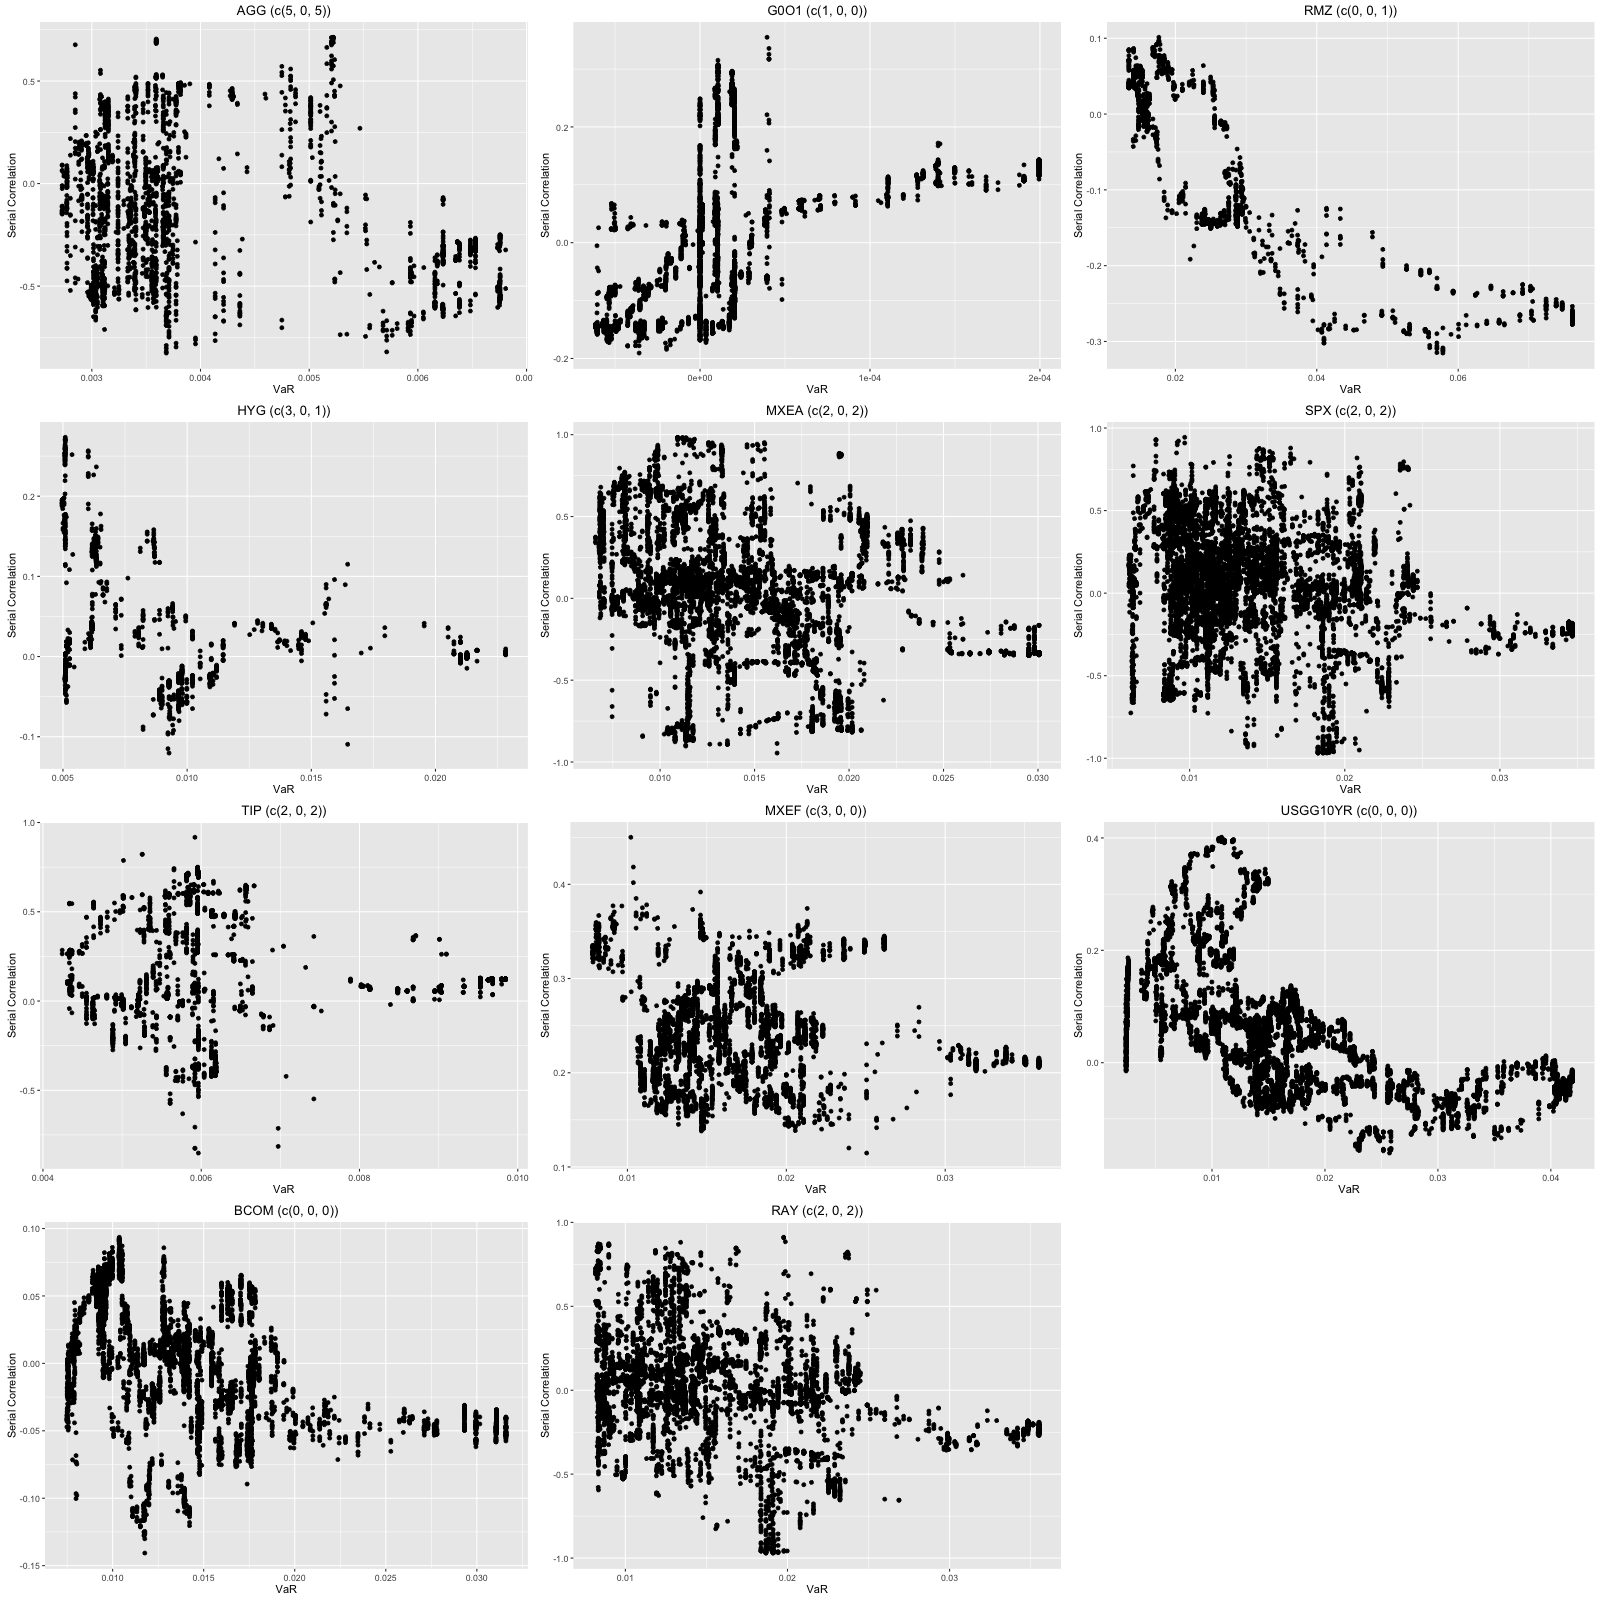
\includegraphics[width = \textwidth]{../figures/SerCol-VaR2yr}
  \label{fig:SerCol-VaR2yr}
\end{figure}

\begin{figure}
  \caption{Relationship First-order Serial Correlation and ES using Best Model}
  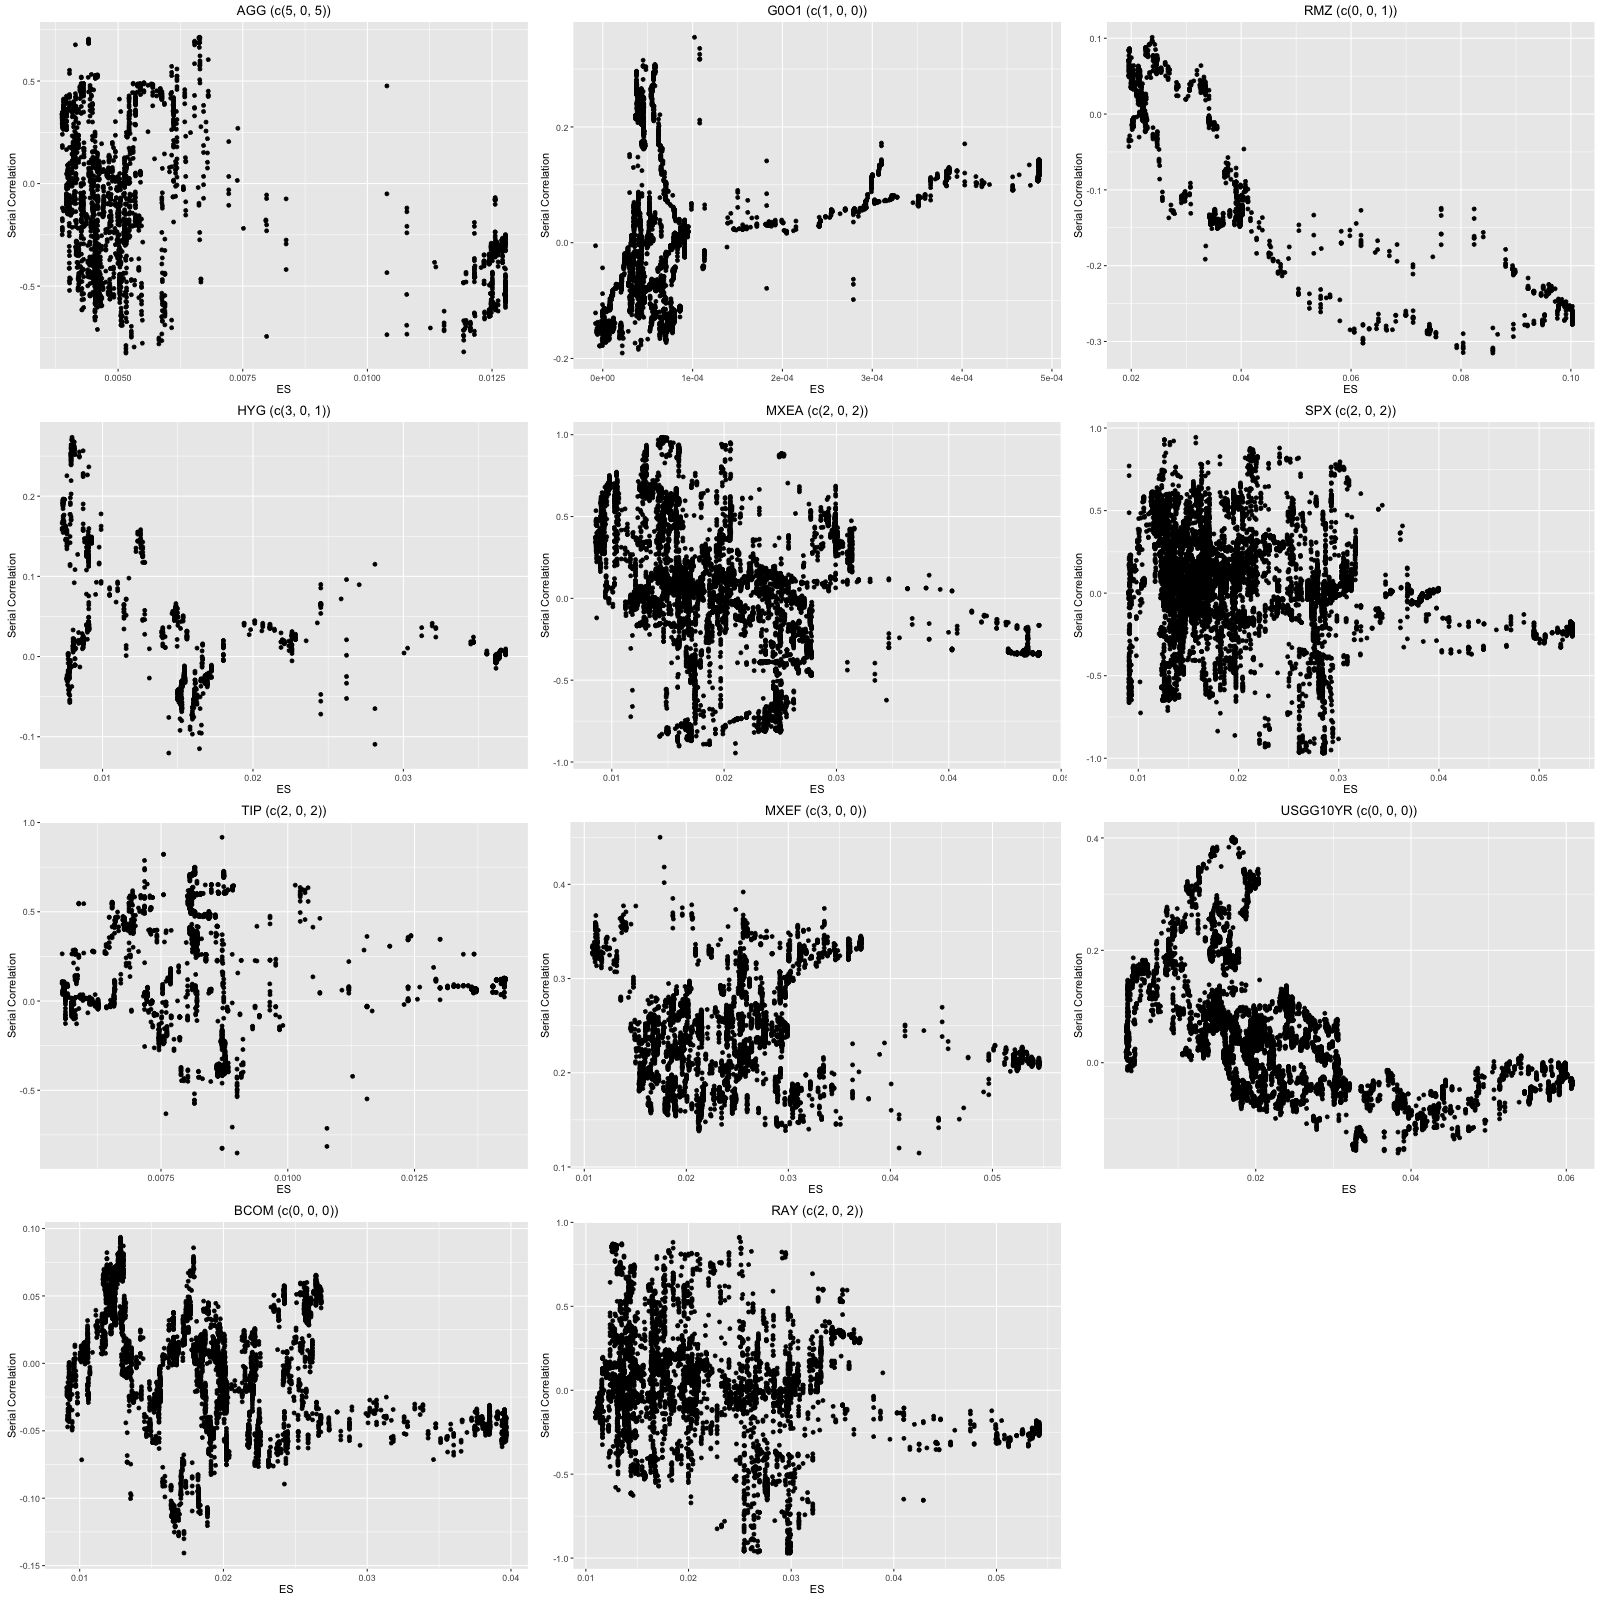
\includegraphics[width = \textwidth]{../figures/SerCol-ES2yr}
  \label{fig:SerCol-ES2yr}
\end{figure}

\begin{figure}
  \caption{Relationship First-order Serial Correlation and CED using Best Model}
  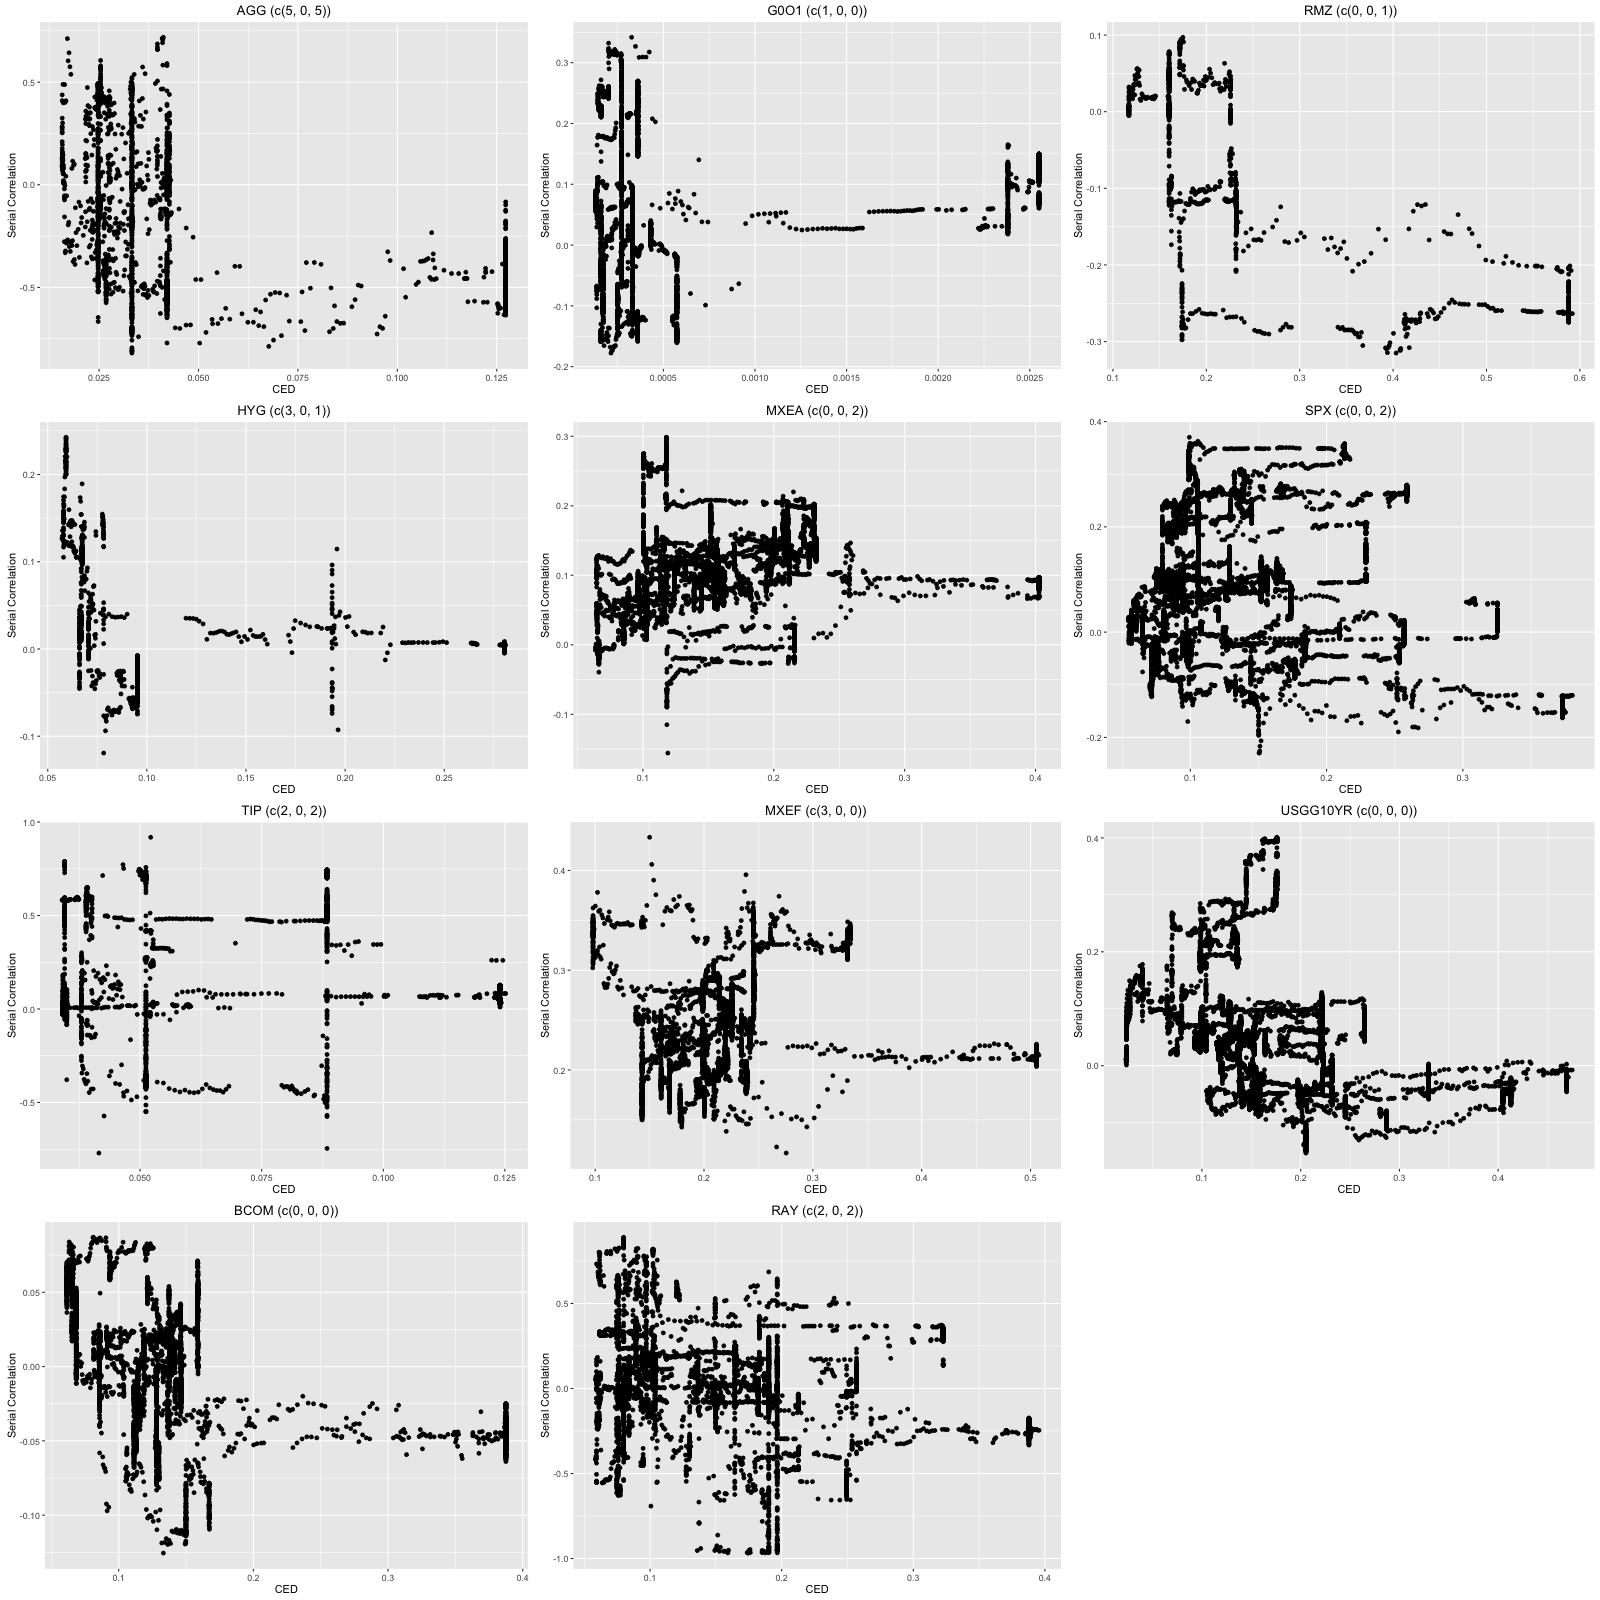
\includegraphics[width = \textwidth]{../figures/SerCol-CED3mon2yr}
  \label{fig:SerCol-CED3mon2yr}
\end{figure}

\begin{table}[!h]
\caption{Correlation between First-order Serial Correlation and Risk Measurements}
\centering 
\begin{tabular}{ | c || r | r | r | r |} 
 \hline
Asset& Model & v.s. VaR & v.s. VaR &v.s. CED\\
  \hline \hline
AGG &ARMA(5,5) &-0.2456 &  -0.3605&-0.3972 \\ 
HYG &ARMA(3,1) & -0.3162& -0.3346 & -0.2419 \\ 
TIP & AR(1)  &-0.0369 & -0.0660 & 0.0286 \\ 
BCOM &AR(1) & -0.4291&  -0.3897& -0.4298\\ 
MXEA & MA(2) &-0.3358&  -0.3542& 0.1402\\ 
MXEF & AR(3)  &-0.0379  &  -0.0084& 0.0958\\ 
RAY & MA(1) &-0.3459 &   -0.2611&  -0.2234\\ 
RMZ & ARMA(2,2) &-0.8621 &  -0.8763&  -0.7949\\ 
SPX & MA(2)  &-0.1983 &  -0.2267& -0.1220\\ 
USGG10YR &  AR(1) &-0.5578&  -0.5168& -0.3866\\
 \hline
\end{tabular}
\label{table:vsRiskMeasure}
\end{table}

\subsubsection{A Small Simulation Study}
We simulated a AR(1) time series and want to take a look at the relationship between risk measurements and serial correlations. The Figure \ref{fig:SimPart2} shows that VaR/ES has a positive relationship with first-order serial correlation. This is strange compared with the conclusion we have got in the previous section, which is in need of deeper analysis.
\begin{figure}
  \caption{Sim AR(1): First-order Serial Correlation and Risk Measurements}
  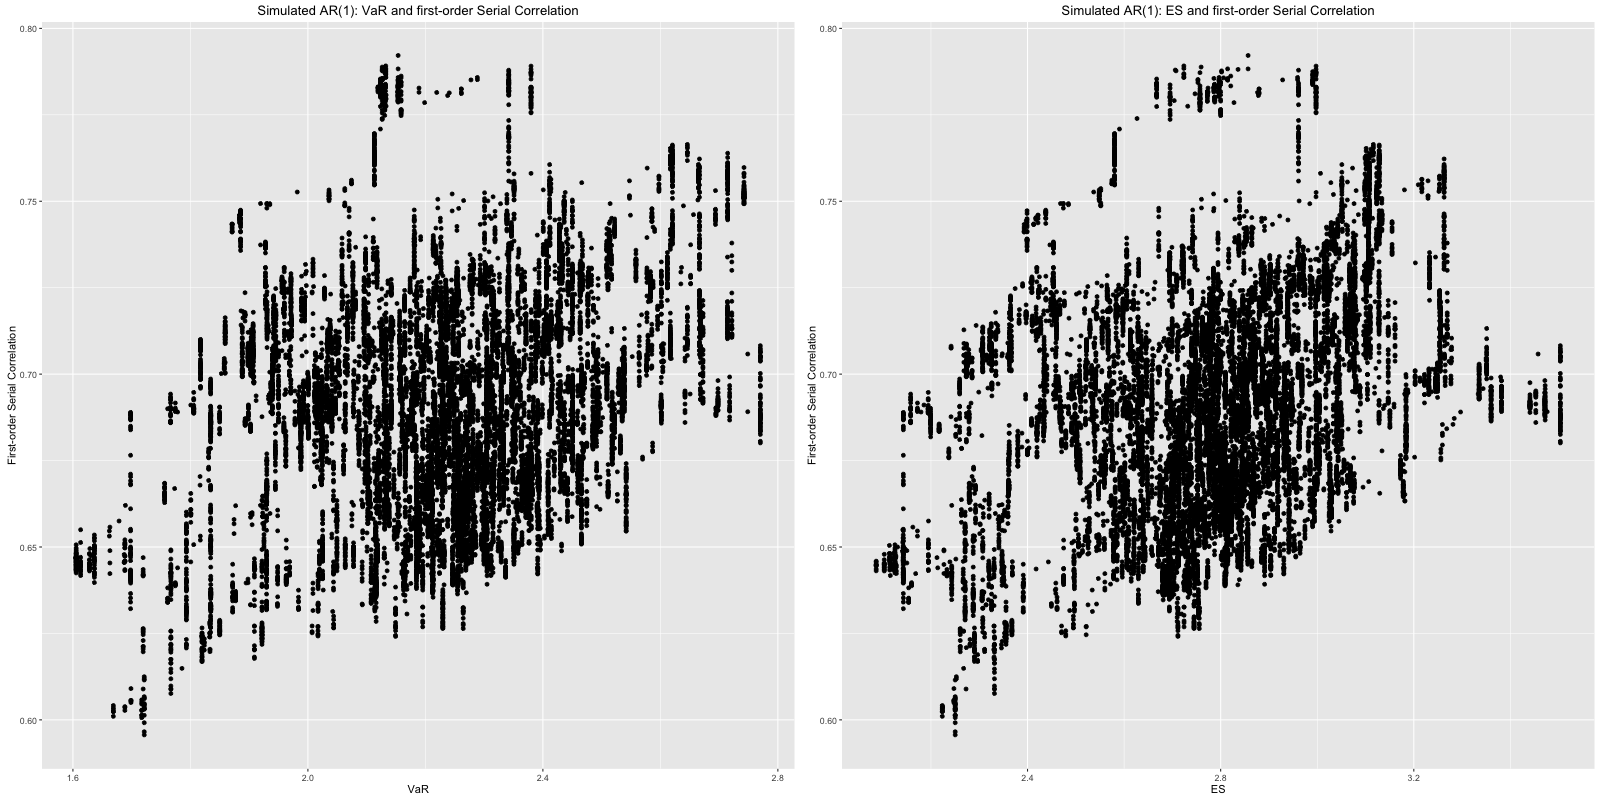
\includegraphics[width = \textwidth]{../figures/sim_part2}
  \label{fig:SimPart2}
\end{figure}
%\end{document}

\clearpage

%%%%%%%%%%%%%%%%%%%%%
\section{Analysis of weekly and monthly return frequencies}%%%%
%%%%%%%%%%%%%%%%%%%%%

\iffalse

%-*- program: xelatex -*-        
%-*- program: biber -*-`        
%-*- program: xelatex -*-
\documentclass[12pt]{article}
\usepackage{amsmath,textcomp,amssymb,geometry,graphicx,enumerate,upquote,color}
\usepackage{hyperref}
\usepackage{float}
\usepackage{tikz}
\usepackage{array}
\usepackage{amsfonts}
\def\Session{Fall 2015}
\usepackage[english]{babel}
\title{Model Selection for the US Indices}
\author{Boying Gong, Xinyue Zhou}
\newenvironment{qparts}{\begin{enumerate}[{(}a{)}]}{\end{enumerate}}
\def\endproofmark{$\Box$}
\newenvironment{proof}{\par{\bf Proof}:}{\endproofmark\smallskip}
\begin{document}
\maketitle

\fi


In this section, we focus on diffrent risk measures under different return frequencies. We're especially interested the behaviour of vaious risk diagnostics under different return frequencies. As we move to longer period such as weekly data, the risk measures such as VaR and ES become unreliable since they are based on the tail of distributions and require a comparatively large amount of dataset. Here we only focused on the comparison of daily and weekly data. 

Figure \ref{fig: mdd_dist_daily_weekly} shows the maximum drawdown distribution of daily (upper panel) and weekly returns (lower panel). Here we use three assets AGG, HYG and TIP as examples. The maximum drawdown distribution of weekly returns are more close to zero and have lighter tails than the distribution of daily returns.

\begin{figure}[h]
\caption{Maximum drawdown (3 month) density of returns based on daily (upper panel) and weekly (lower panel) frequencies} 
\centering 
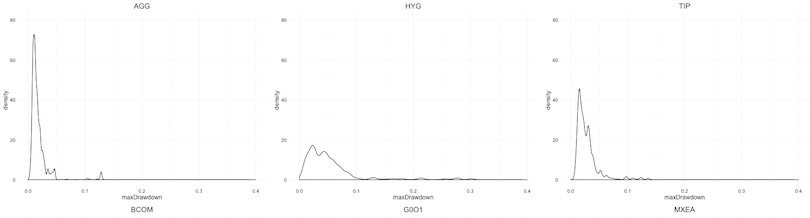
\includegraphics[width=0.9\textwidth]{../figures/maxDrawdown_CED/daily_mdd}
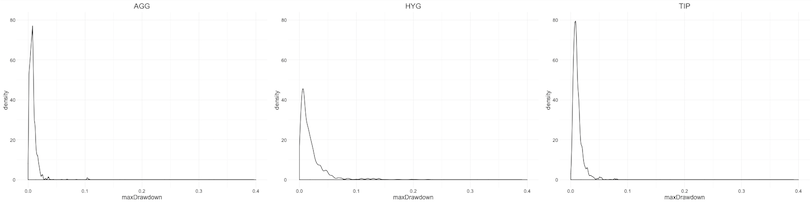
\includegraphics[width=0.9\textwidth]{../figures/maxDrawdown_CED/weekly_mdd}
\label{fig: mdd_dist_daily_weekly}
\end{figure}

We now move to other risk mesures. As we can see from last several sections, ES, VaR and volatility are every closely related. Here I use expected shortfall as an illustration. Figure \ref{fig: ES_daily_weekly_monthly} shows the ES values based on daily (upper panel), weekly (midlle panel) and monthly (lower panel) frequencies. As we expected, there are missing values for the tail mean when we move to longer period such as monthly data. The values of ES of weekly data are nearly as twice as the daily data since they are based on weeekly returns. However, after annualizing the returns, we can see that the number calculated using weekly reeturns are actually smaller. This phenomenon is more obvious when we move to monthly data. The ES calculated using annualized monthly returns are even smaller than its weekly counterpart.

\begin{figure}[h]
\caption{ES (6 month) based on daily (upper panel), weekly (midlle panel) and monthly (lower panel) frequencies} 
\centering 
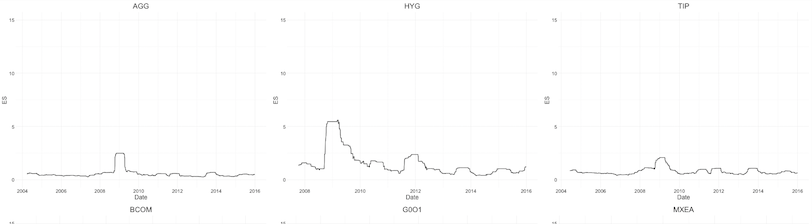
\includegraphics[width=0.9\textwidth]{../figures/rolling_stats/daily_ES}
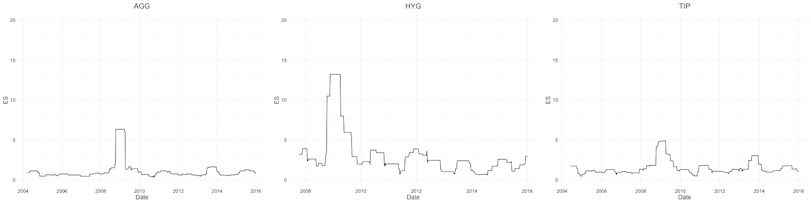
\includegraphics[width=0.9\textwidth]{../figures/rolling_stats/weekly_ES}
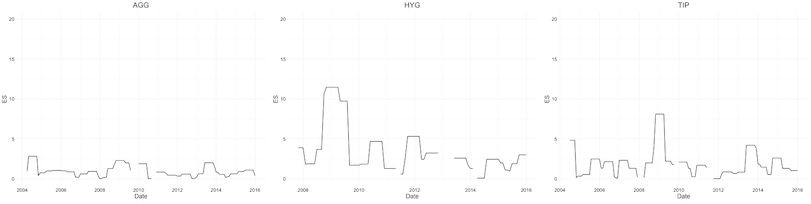
\includegraphics[width=0.9\textwidth]{../figures/rolling_stats/monthly_ES}
\label{fig: ES_daily_weekly_monthly}
\end{figure}



%\end{document}


\clearpage

%%%%%%%%%%%%%%%%%%%%%
\section{Appendix: Plot and Tables}%%%
%%%%%%%%%%%%%%%%%%%%%

\begin{figure}[h]
\caption{Daily Returns} 
\centering 
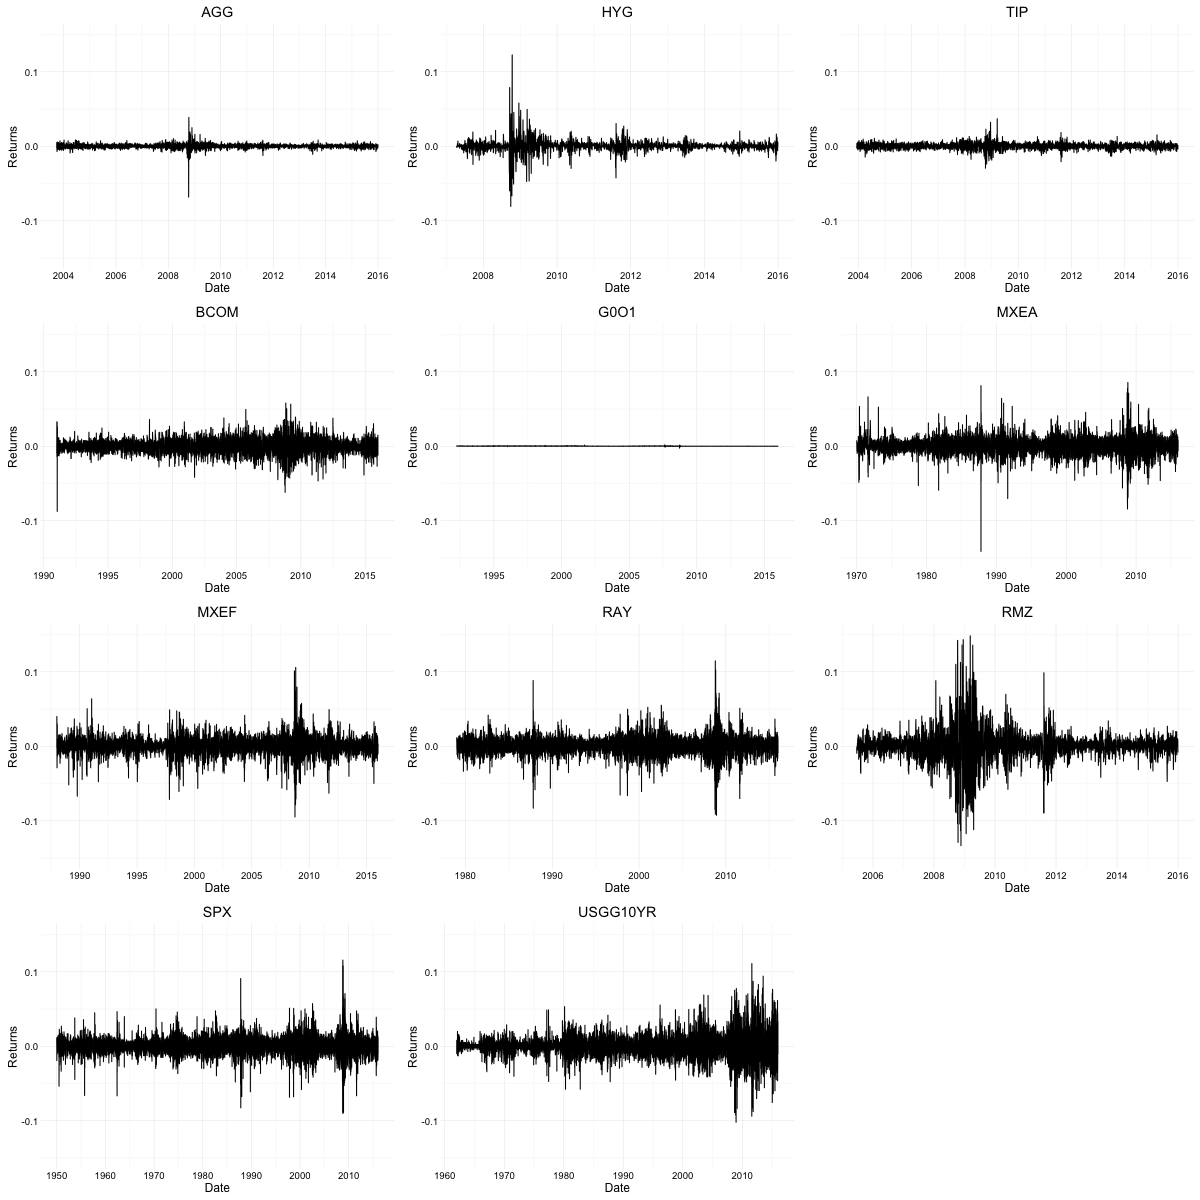
\includegraphics[width=15cm]{../figures/summary_daily/returns}
\label{fig: dailyReturns}
\end{figure}

\begin{figure}[h]
\caption{Empirical distribution of daily returns} 
\centering 
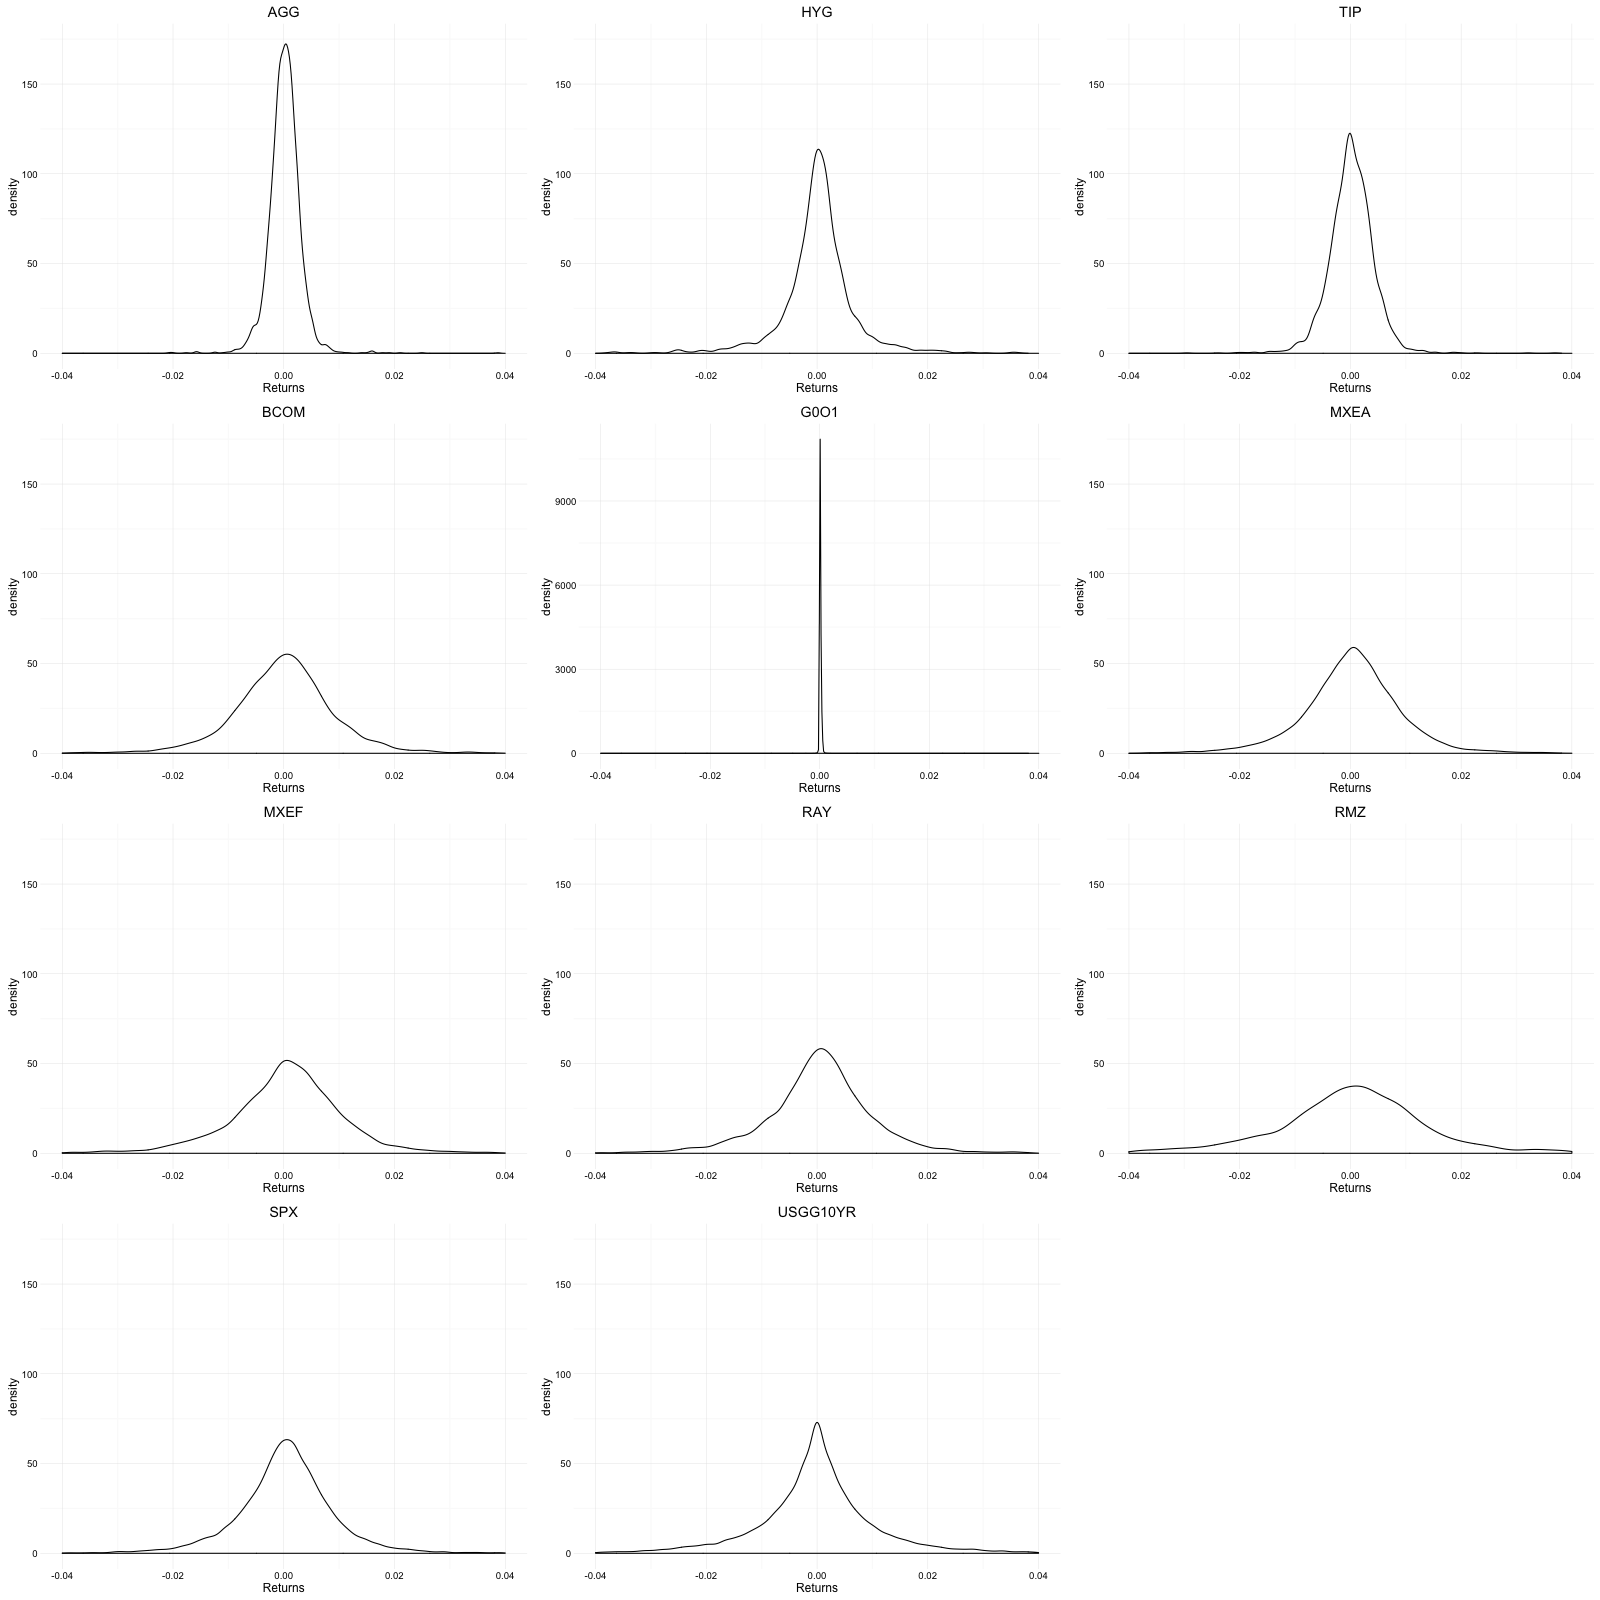
\includegraphics[width=15cm]{../figures/summary_daily/returns_dist}
\label{fig: returnsDist}
\end{figure}

\begin{figure}[h]
\caption{Empirical distribution of maximum drawdown under 3 month rolling window} 
\centering
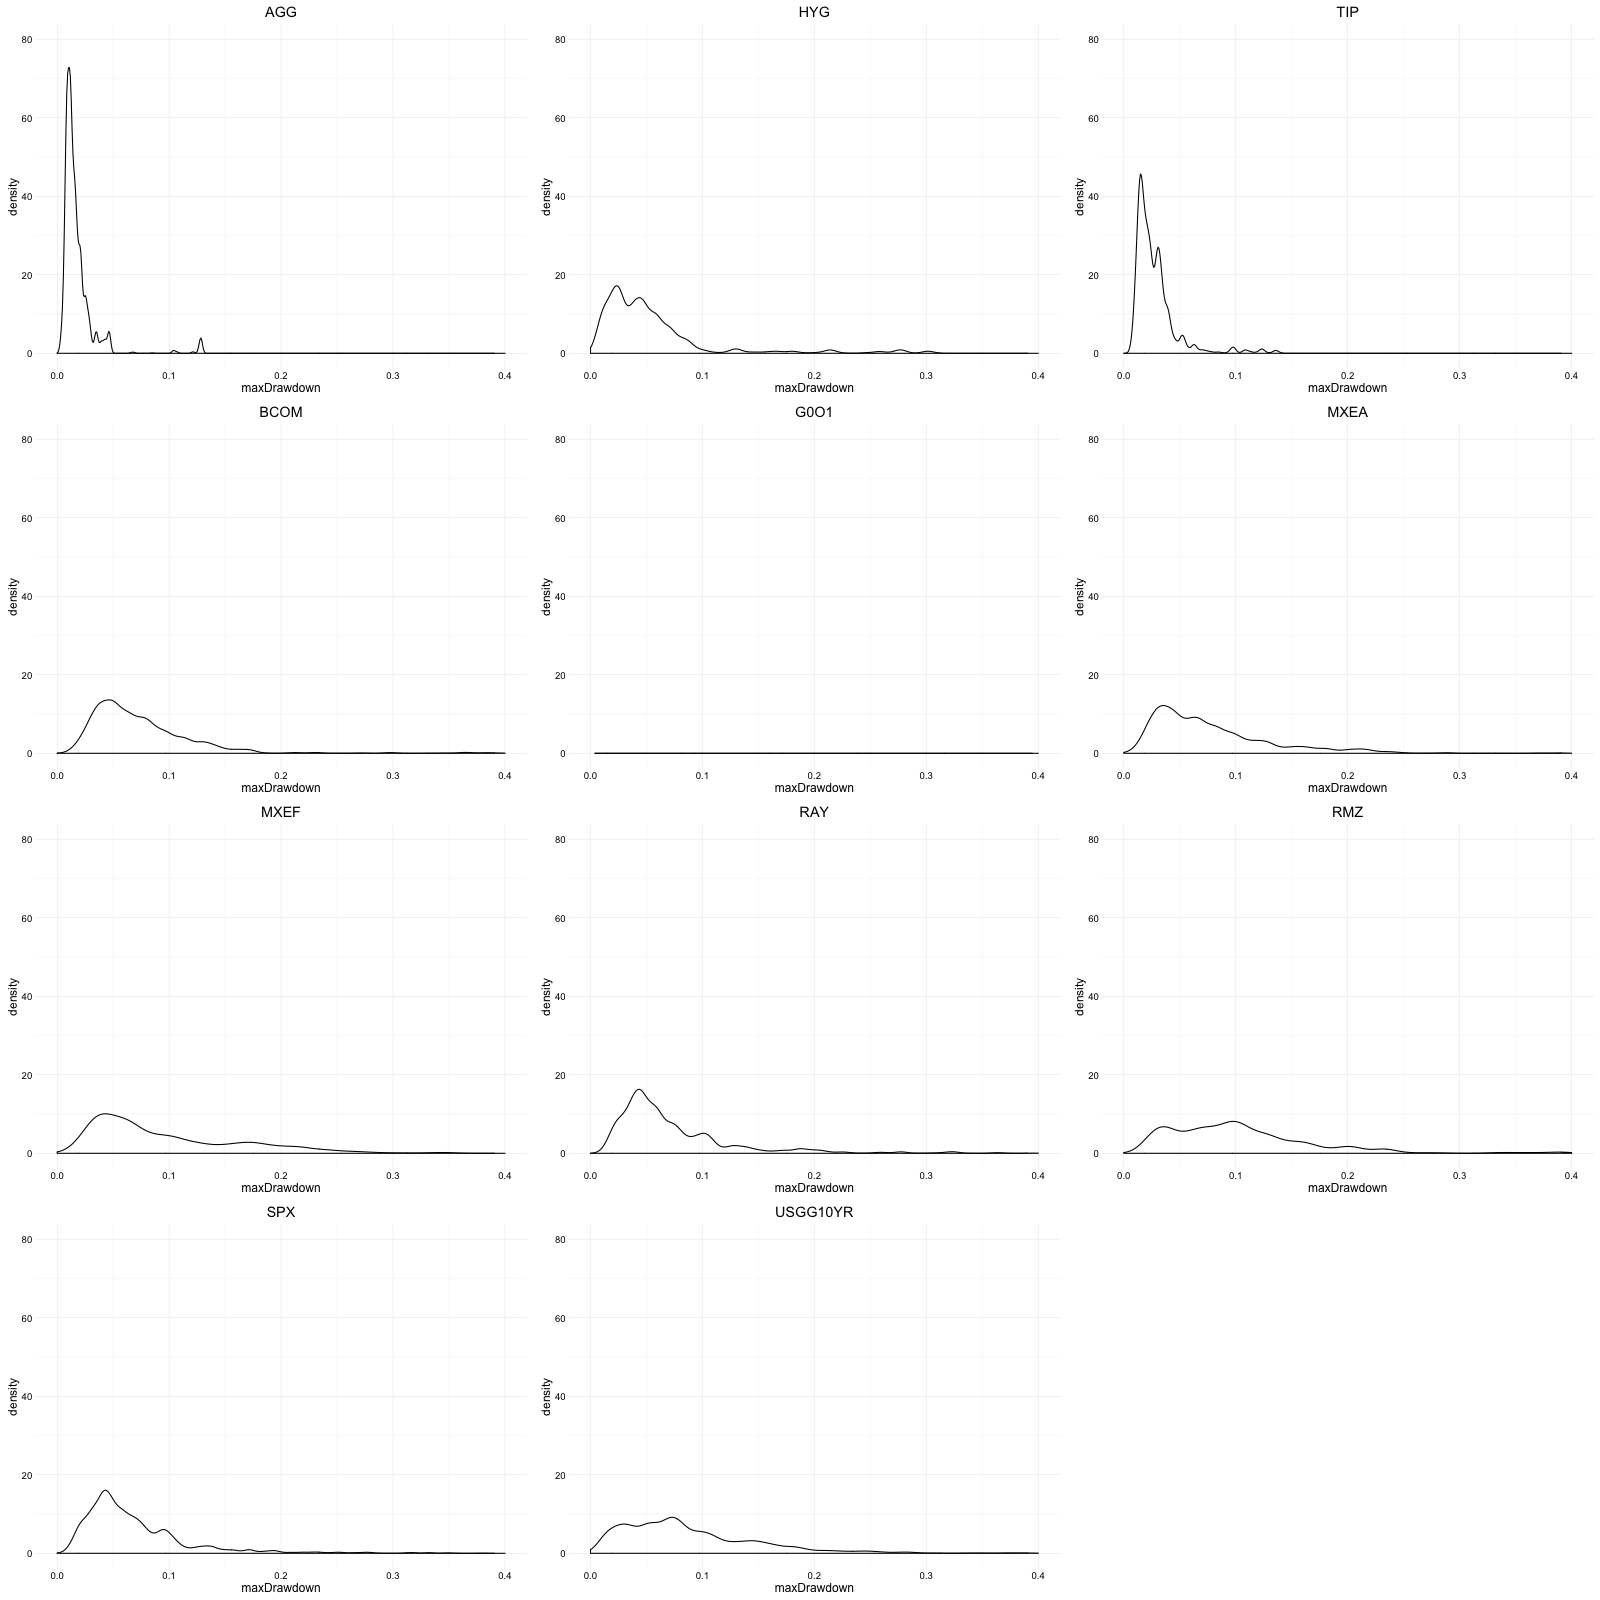
\includegraphics[width=15cm]{../figures/maxDrawdown_CED/maxDrawdown3mon}
\label{fig: dist_mdd}
\end{figure}

\begin{table}[!h]
\centering 
\caption{tail mean of maximum drawdown distribution under 3-month, 6-month, 1-year and 2-year rolling window} 
\begin{tabular}{ | r || r r r || r r r |} 
 \hline
 & & 3 month & & & 6 month & \\
Asset& 0.9 & 0.95 & 0.99 & 0.9 & 0.95 & 0.99  \\
  \hline \hline
AGG &  5.60 &  7.72 & 12.84 &  8.12 & 11.45 & 12.84\\ 
HYG & 18.41 & 24.07 & 29.67 & 26.43 & 30.77 & 32.26\\ 
TIP &  7.48 &  9.90 & 13.10 & 11.14 & 12.91 & 14.39\\ 
BCOM & 18.14 & 22.54 & 38.03 & 26.61 & 33.66 & 51.74\\ 
G0O1 &  0.10 &  0.145 &  0.26 &  0.14 &  0.23 &  0.26\\ 
MXEA & 20.39 & 23.73 & 33.32 & 27.21 & 31.79 & 47.11\\ 
MXEF & 26.21 & 30.80 & 48.03 & 36.35 & 43.30 & 59.63\\ 
RAY & 20.65 & 25.64 & 35.95 & 27.81 & 34.08 & 45.08\\ 
RMZ & 37.30 & 48.41 & 63.45 & 52.04 & 62.41 & 67.61\\ 
SPX & 18.35 & 22.67 & 32.46 & 25.18 & 30.65 & 40.69\\ 
USGG10YR & 23.28 & 28.11 & 41.83 & 32.78 & 39.00 & 49.28\\
 \hline \hline
 & & 1 year & & & 2 year & \\
Asset& 0.9 & 0.95 & 0.99 & 0.9 & 0.95 & 0.99  \\
  \hline \hline
AGG & 12.11 & 12.84 & 12.84 & 12.84 & 12.84 & 12.83\\ 
HYG & 33.15 & 34.20 &      & 34.24 & 34.25 &       \\ 
TIP & 13.73 & 14.50 & 14.57 & 14.57 & 14.57 &       \\ 
BCOM & 39.91 & 49.26 & 57.14 & 53.38 & 57.14 &       \\ 
G0O1 &  0.23 &  0.25 &  0.26 &  0.26 &  0.26 &  0.26\\ 
MXEA & 36.15 & 42.61 & 56.70 & 50.21 & 58.08 & 61.85\\ 
MXEF & 48.63 & 58.81 & 64.56 & 62.45 & 65.90 &       \\ 
RAY & 37.56 & 44.06 & 52.42 & 47.95 & 54.33 &       \\ 
RMZ & 67.09 & 69.86 & 70.02 & 73.70 & 74.56 & 74.92\\ 
SPX & 34.07 & 39.15 & 50.30 & 44.62 & 50.47 & 56.77\\ 
USGG10YR & 42.88 & 48.37 & 53.96 & 54.79 & 59.14 & 62.82\\
 \hline
\end{tabular}
\label{table:tail_maxdrawdown}
\end{table}

\begin{figure}[h]
\caption{Volatility under 6-month rolling window} 
\centering 
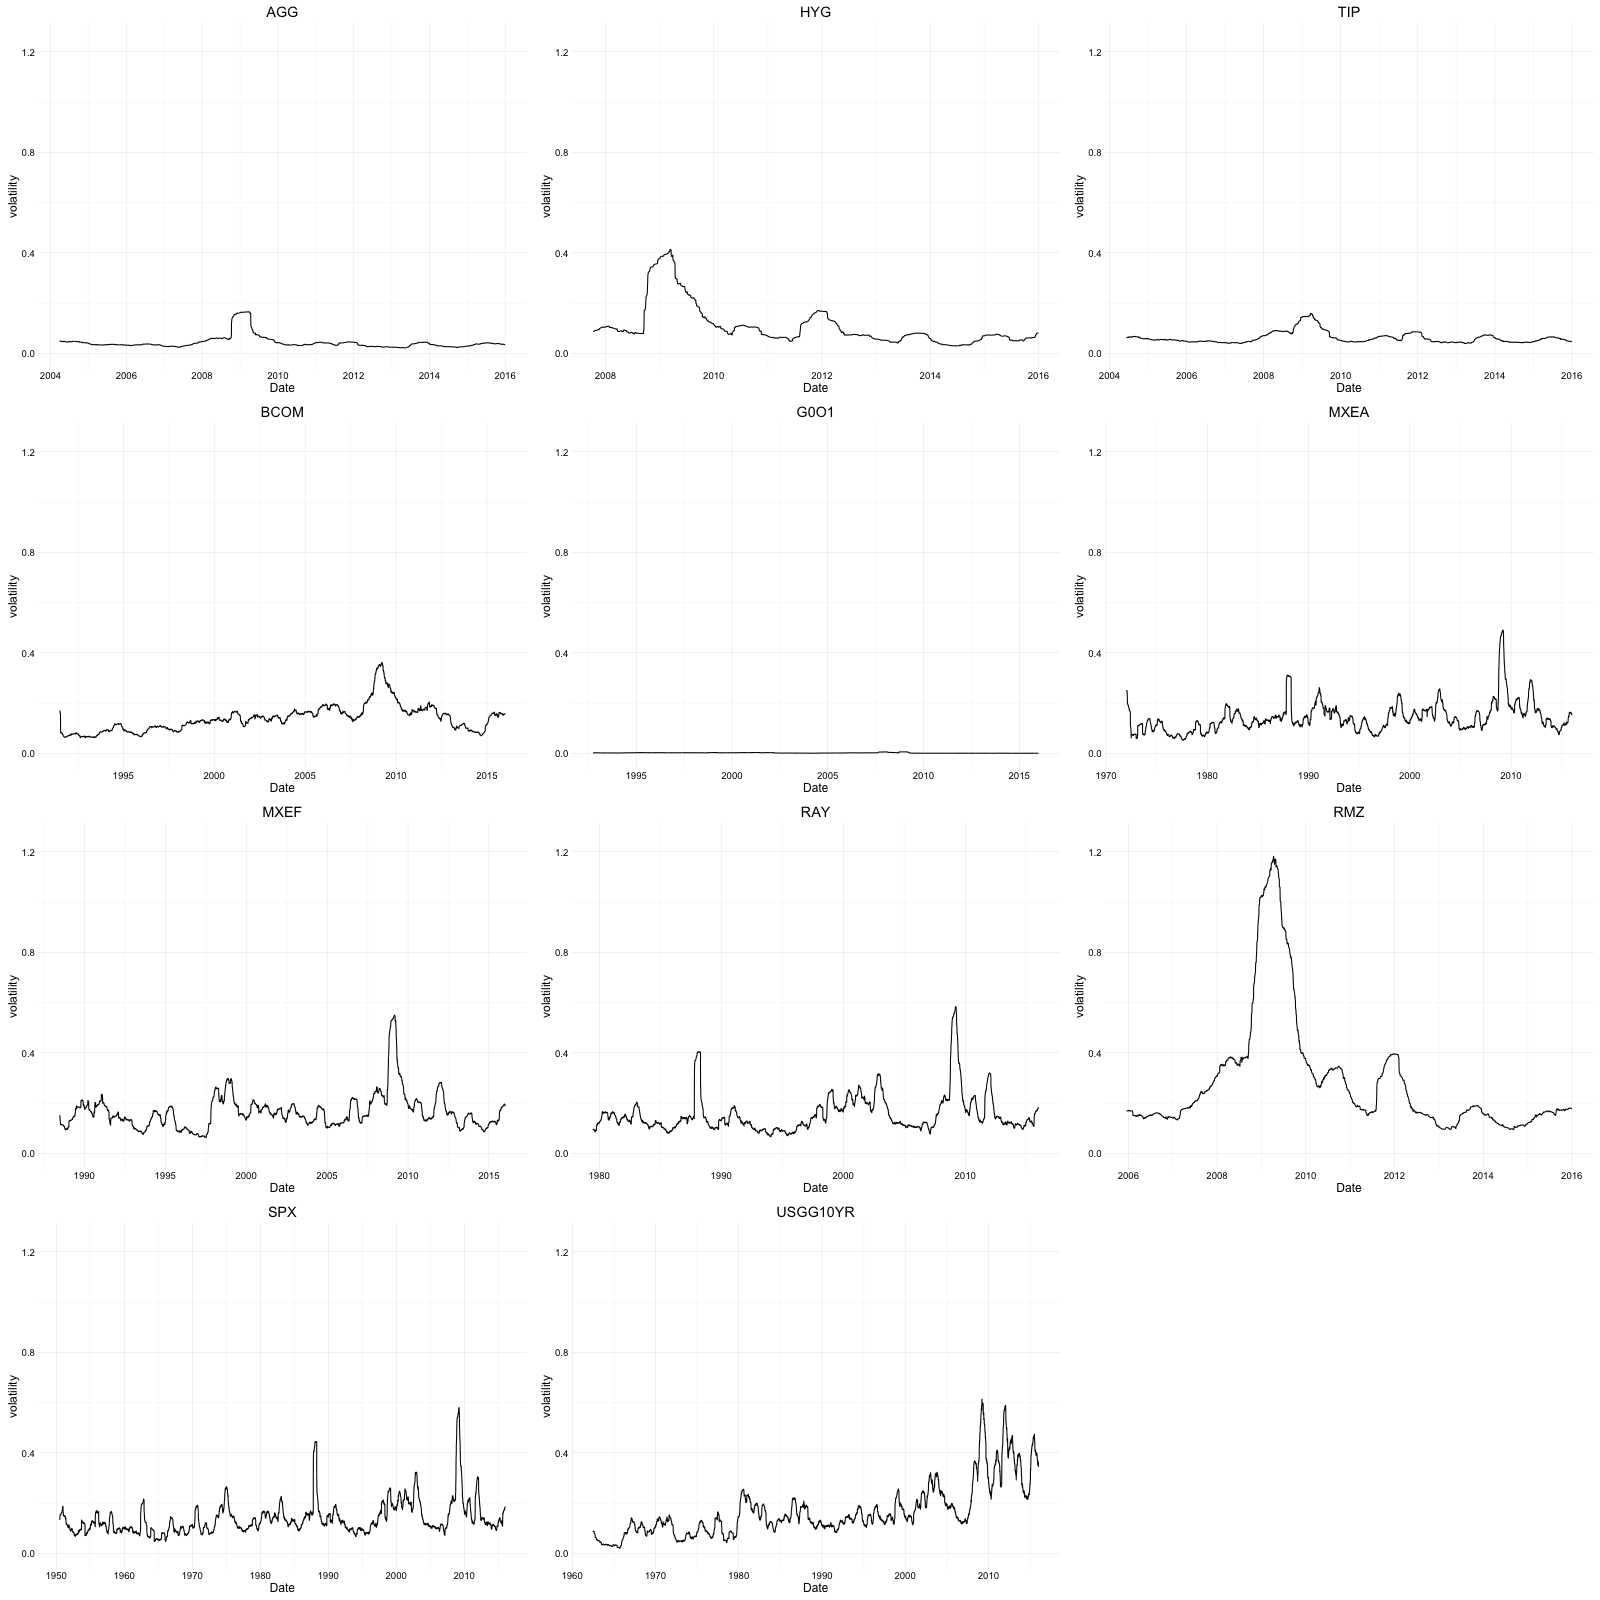
\includegraphics[width=15cm]{../figures/rolling_stats/volatility6mon_scaled}
\label{fig: variance6mon}
\end{figure}

\begin{figure}[h]
\caption{VaR(\%) (significance level = 0.95) under 6-month rolling window}
\centering 
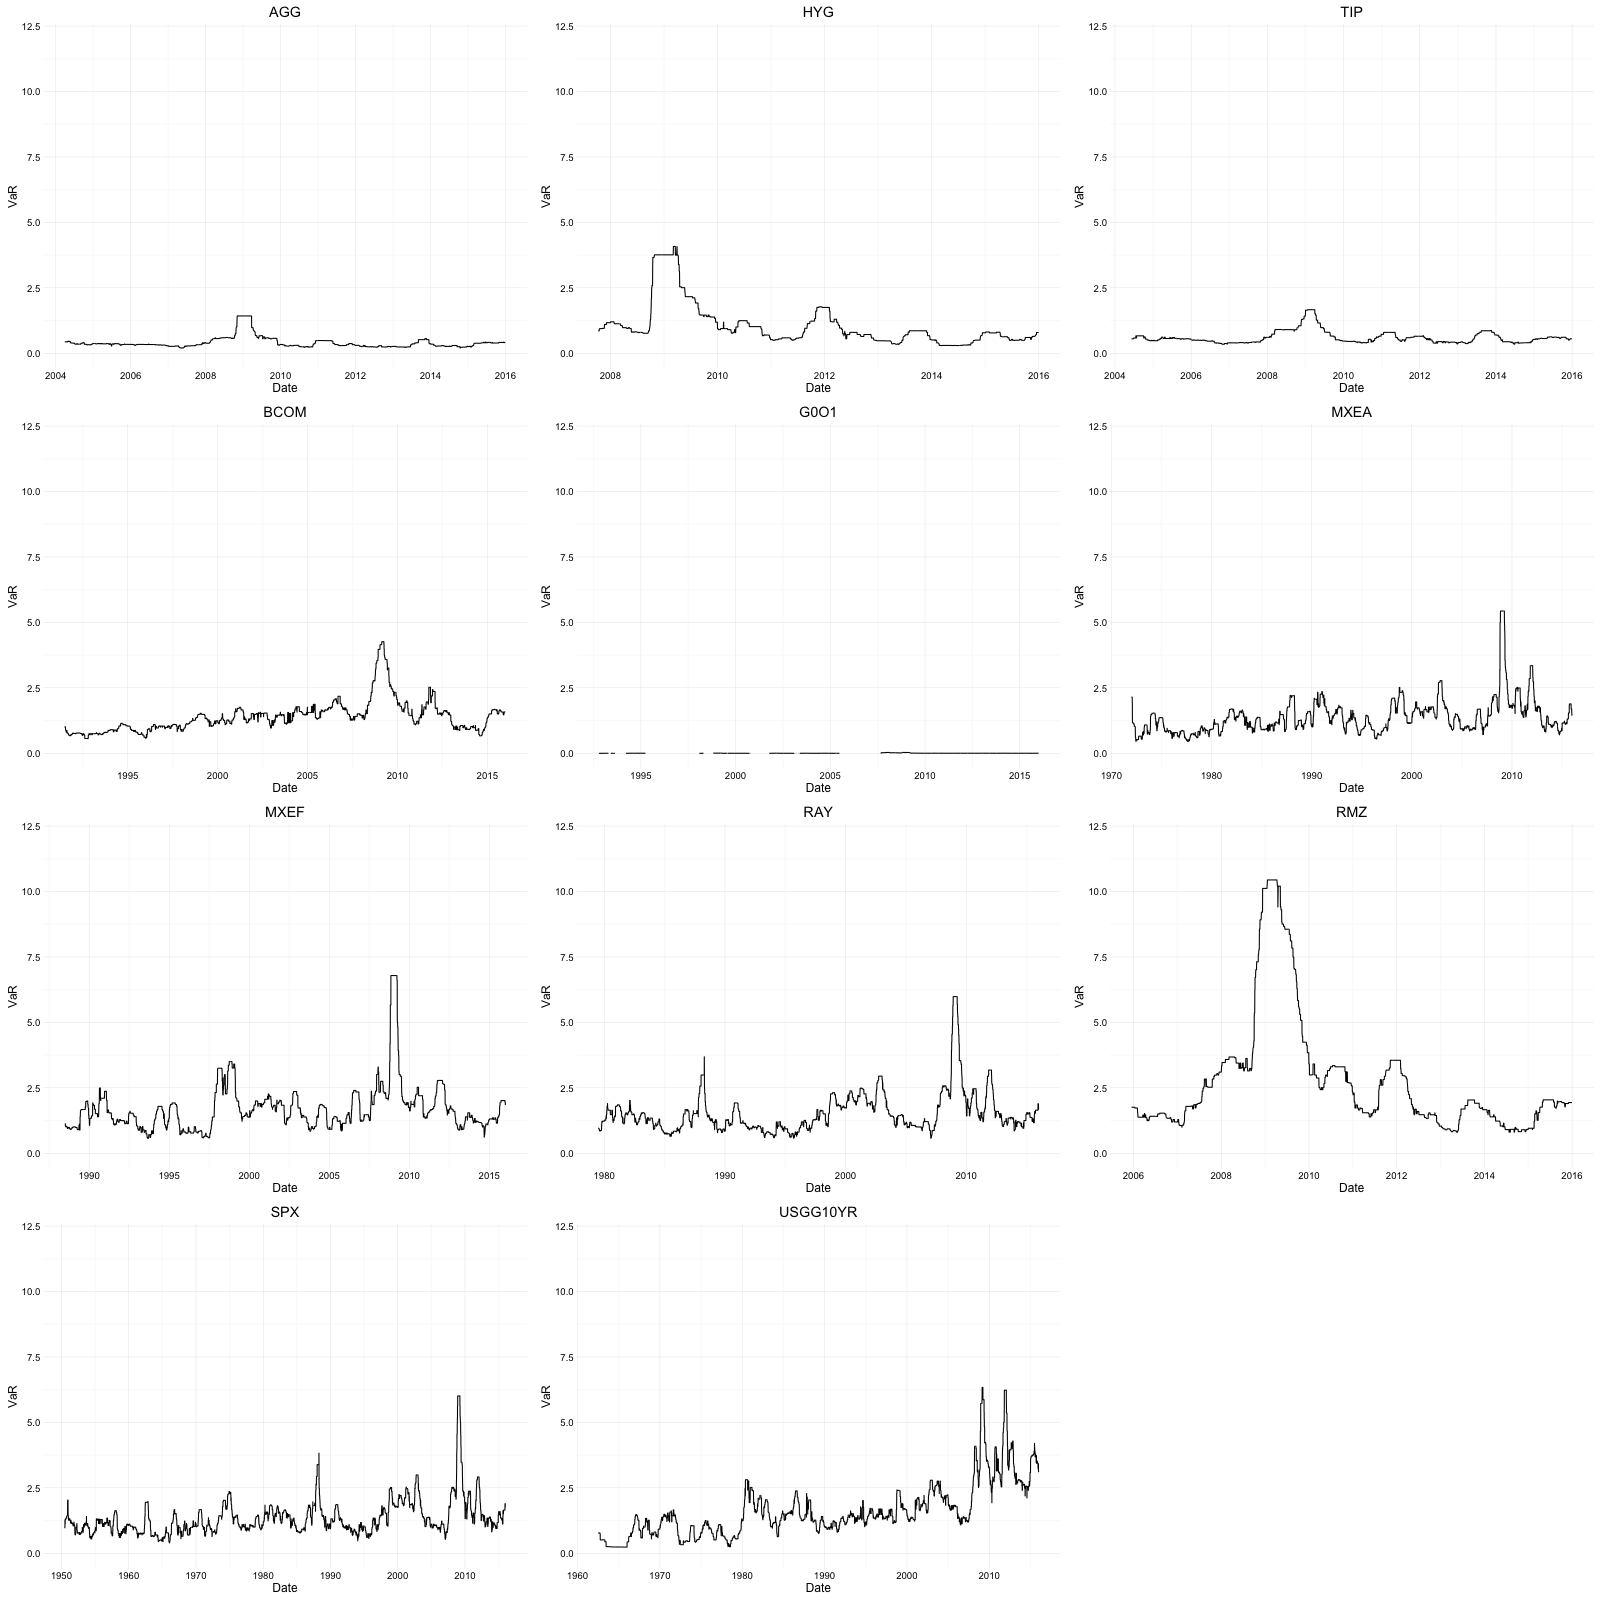
\includegraphics[width=15cm]{../figures/rolling_stats/VaR6mon_scaled}
\label{fig: VaR6mon}
\end{figure}

\begin{figure}[h]
\caption{ES(\%) (significance level = 0.95) under 6-month rolling window} 
\centering 
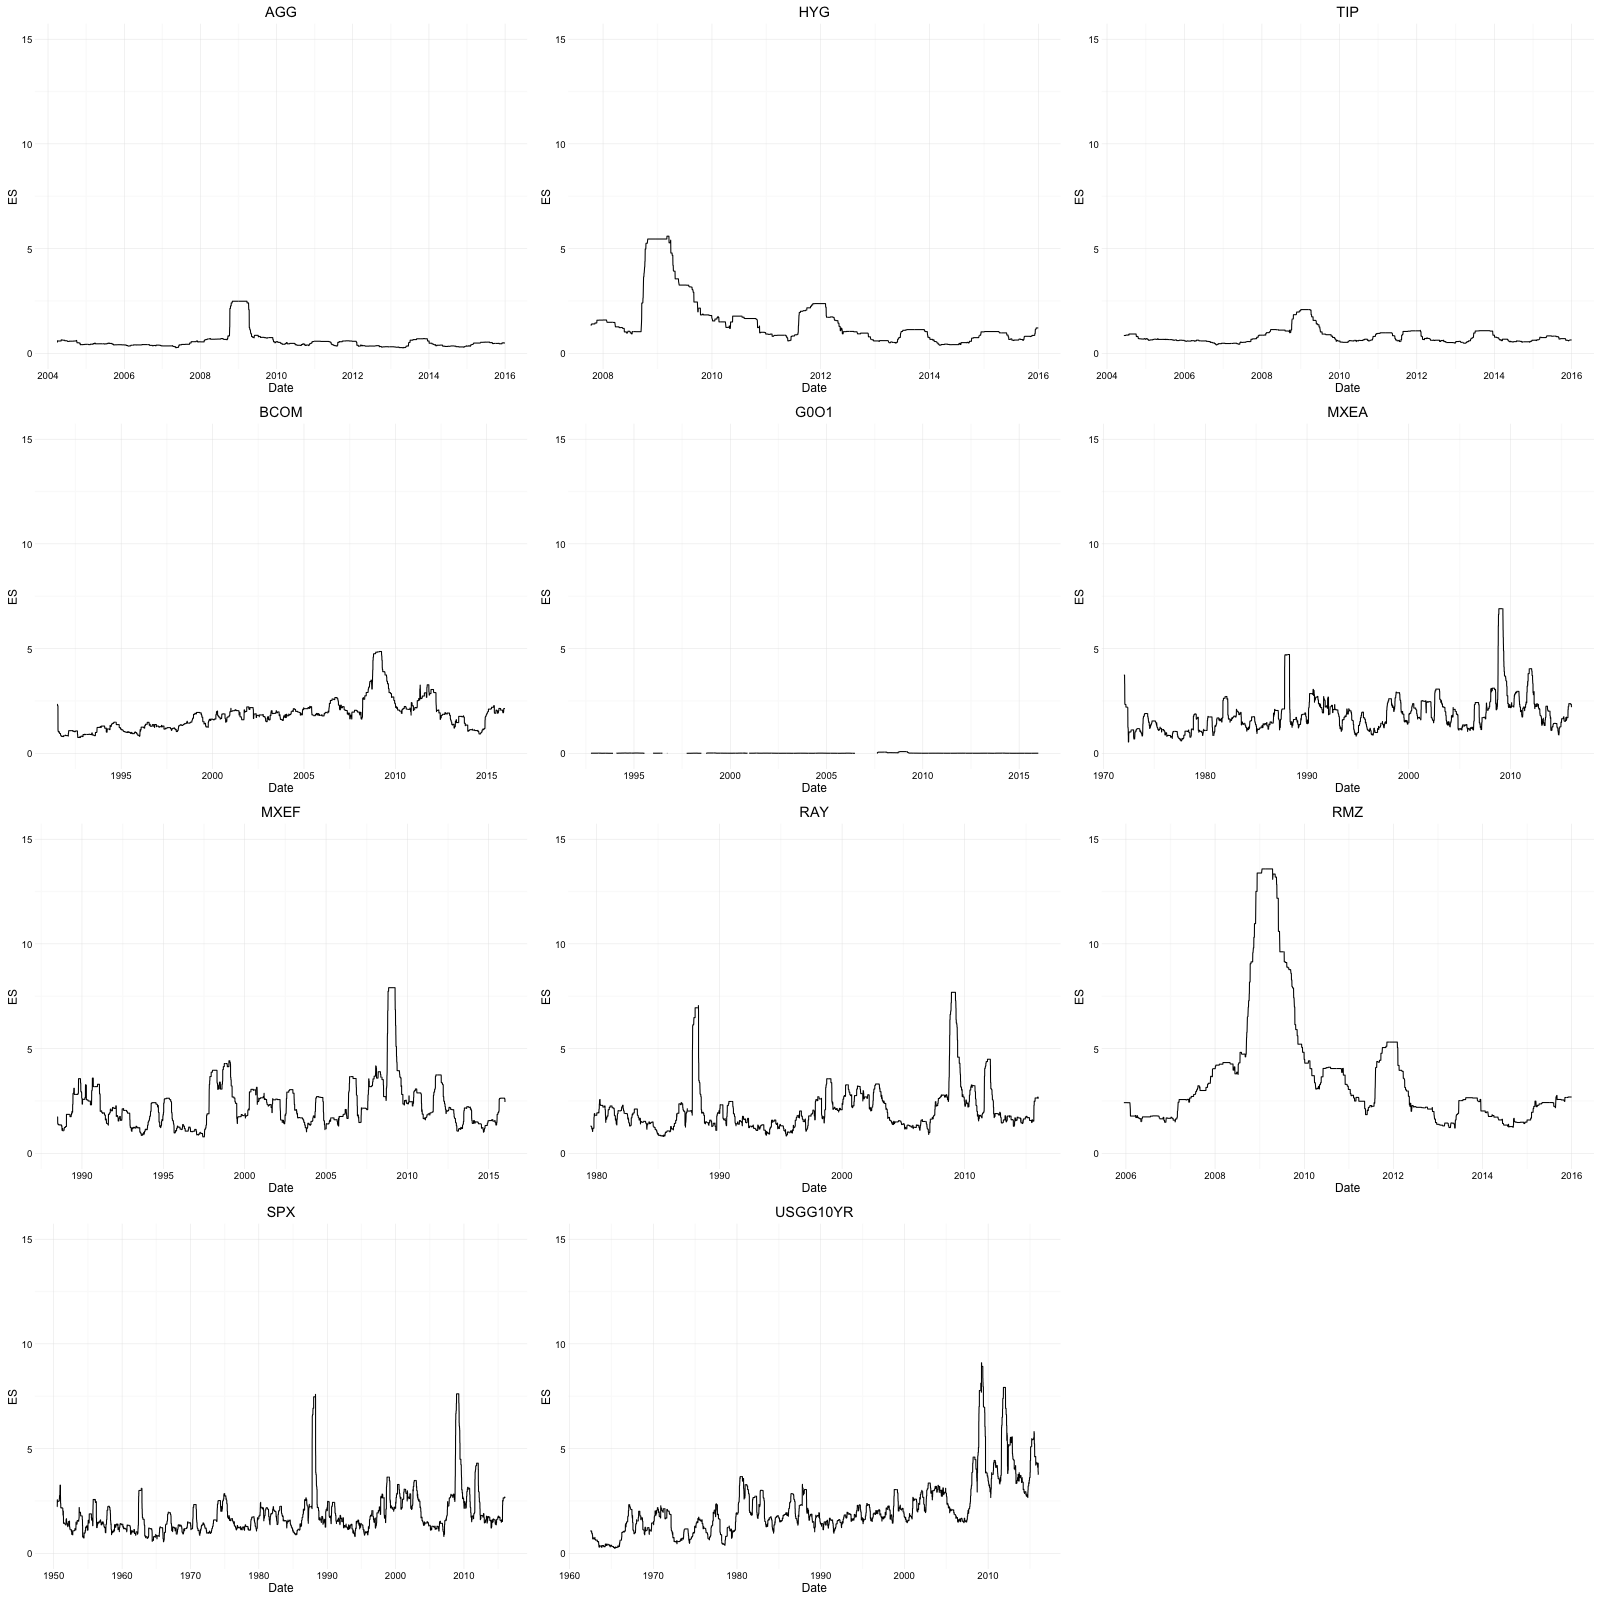
\includegraphics[width=15cm]{../figures/rolling_stats/ES6mon_scaled}
\label{fig: ES6mon}
\end{figure}

\begin{figure}[h]
\caption{CED under 3-month-5-year Rolling Window (confidence level = 0.9)} 
\centering 
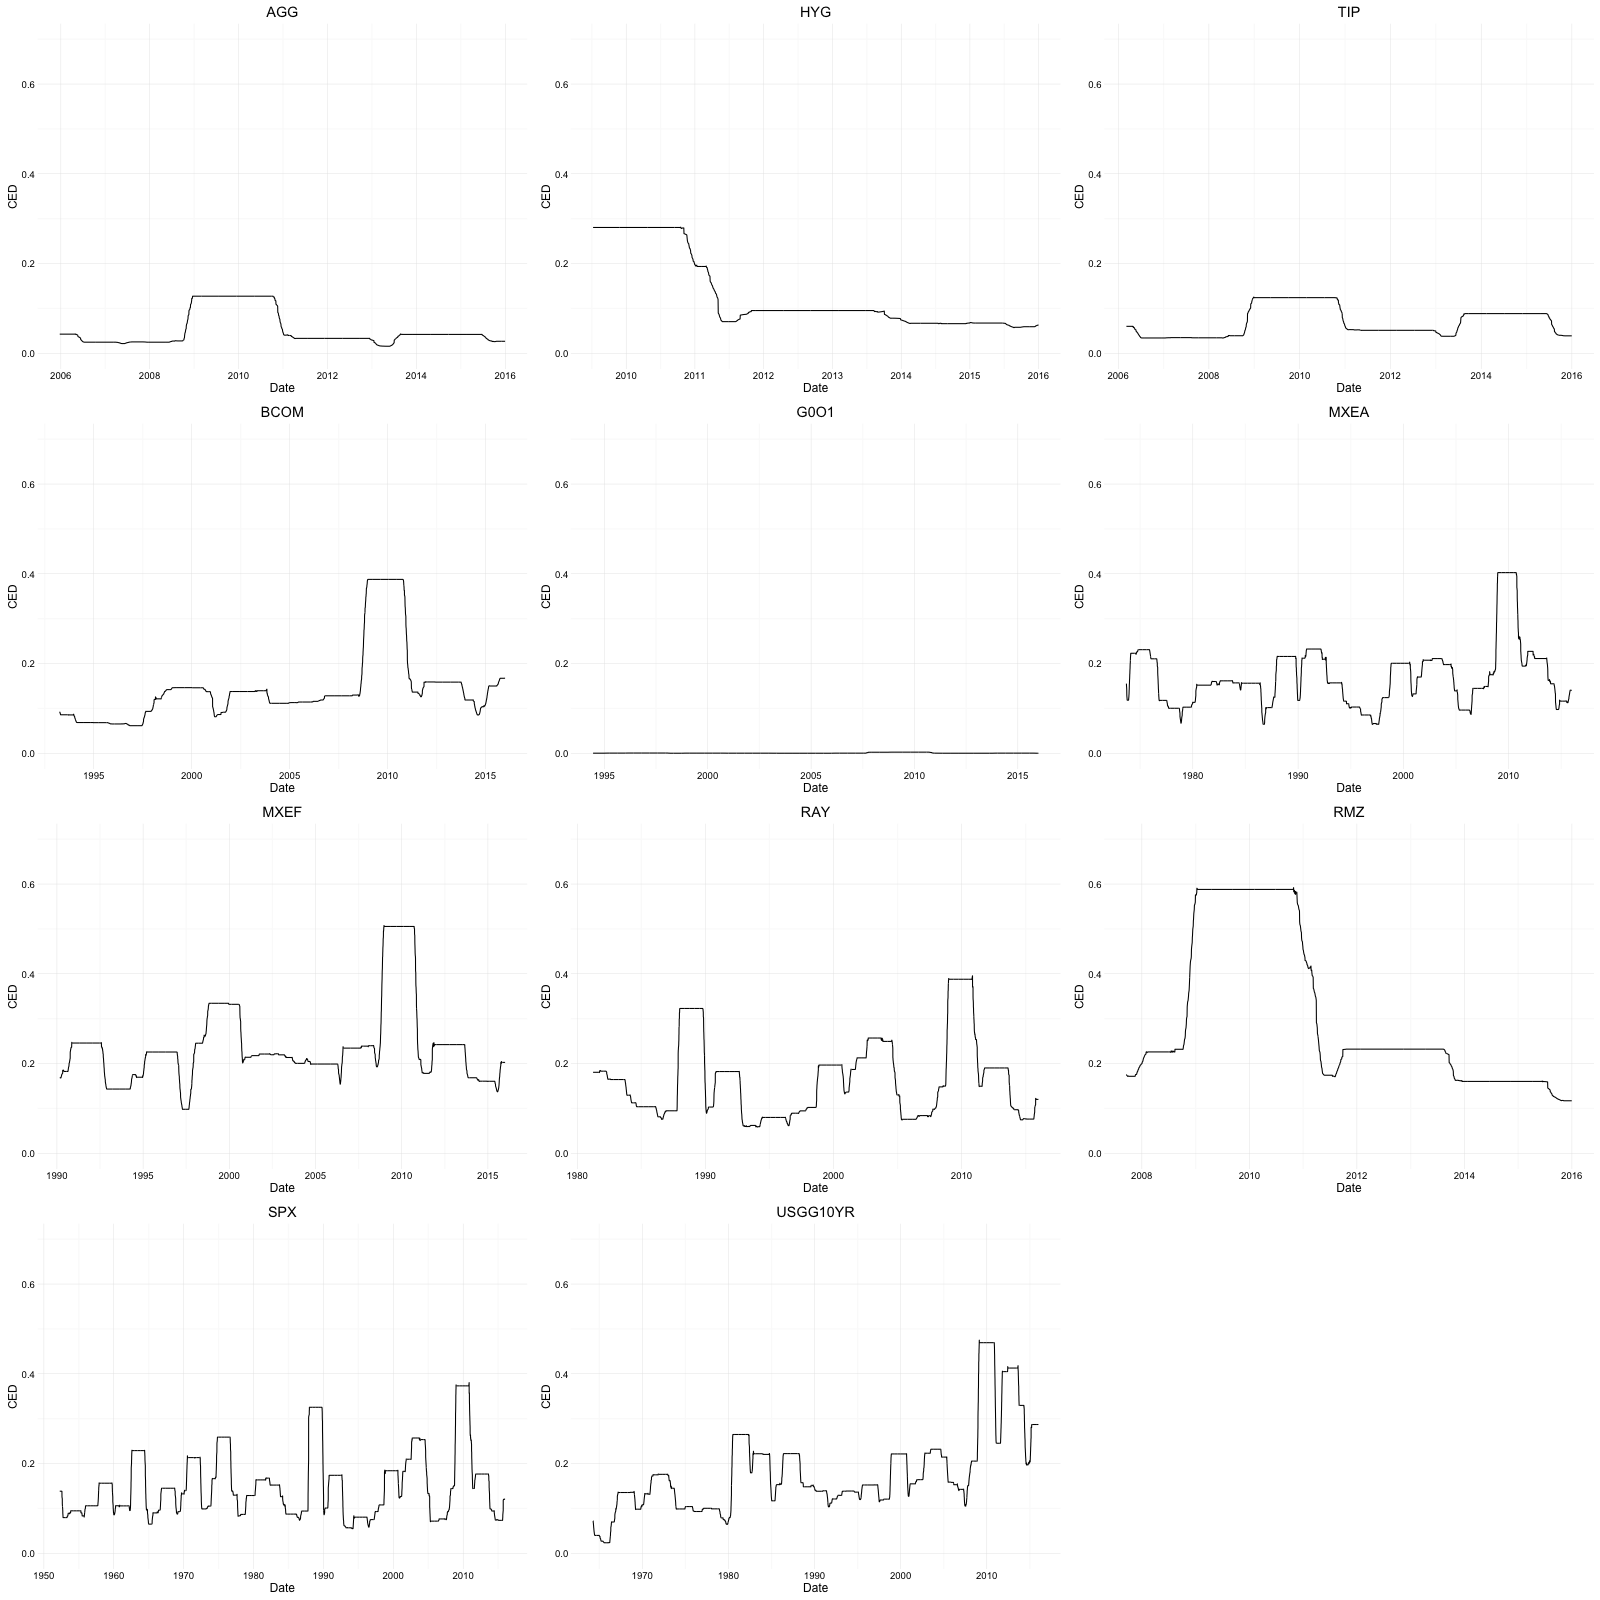
\includegraphics[width=15cm]{../figures/rolling_stats/CED3mon2yr_scaled}
\label{fig: CED3mon2yr}
\end{figure}

\begin{figure}[h]
\caption{CED (confidence level = 0.9) versus ES under 3-month-2-year Rolling Window} 
\centering 
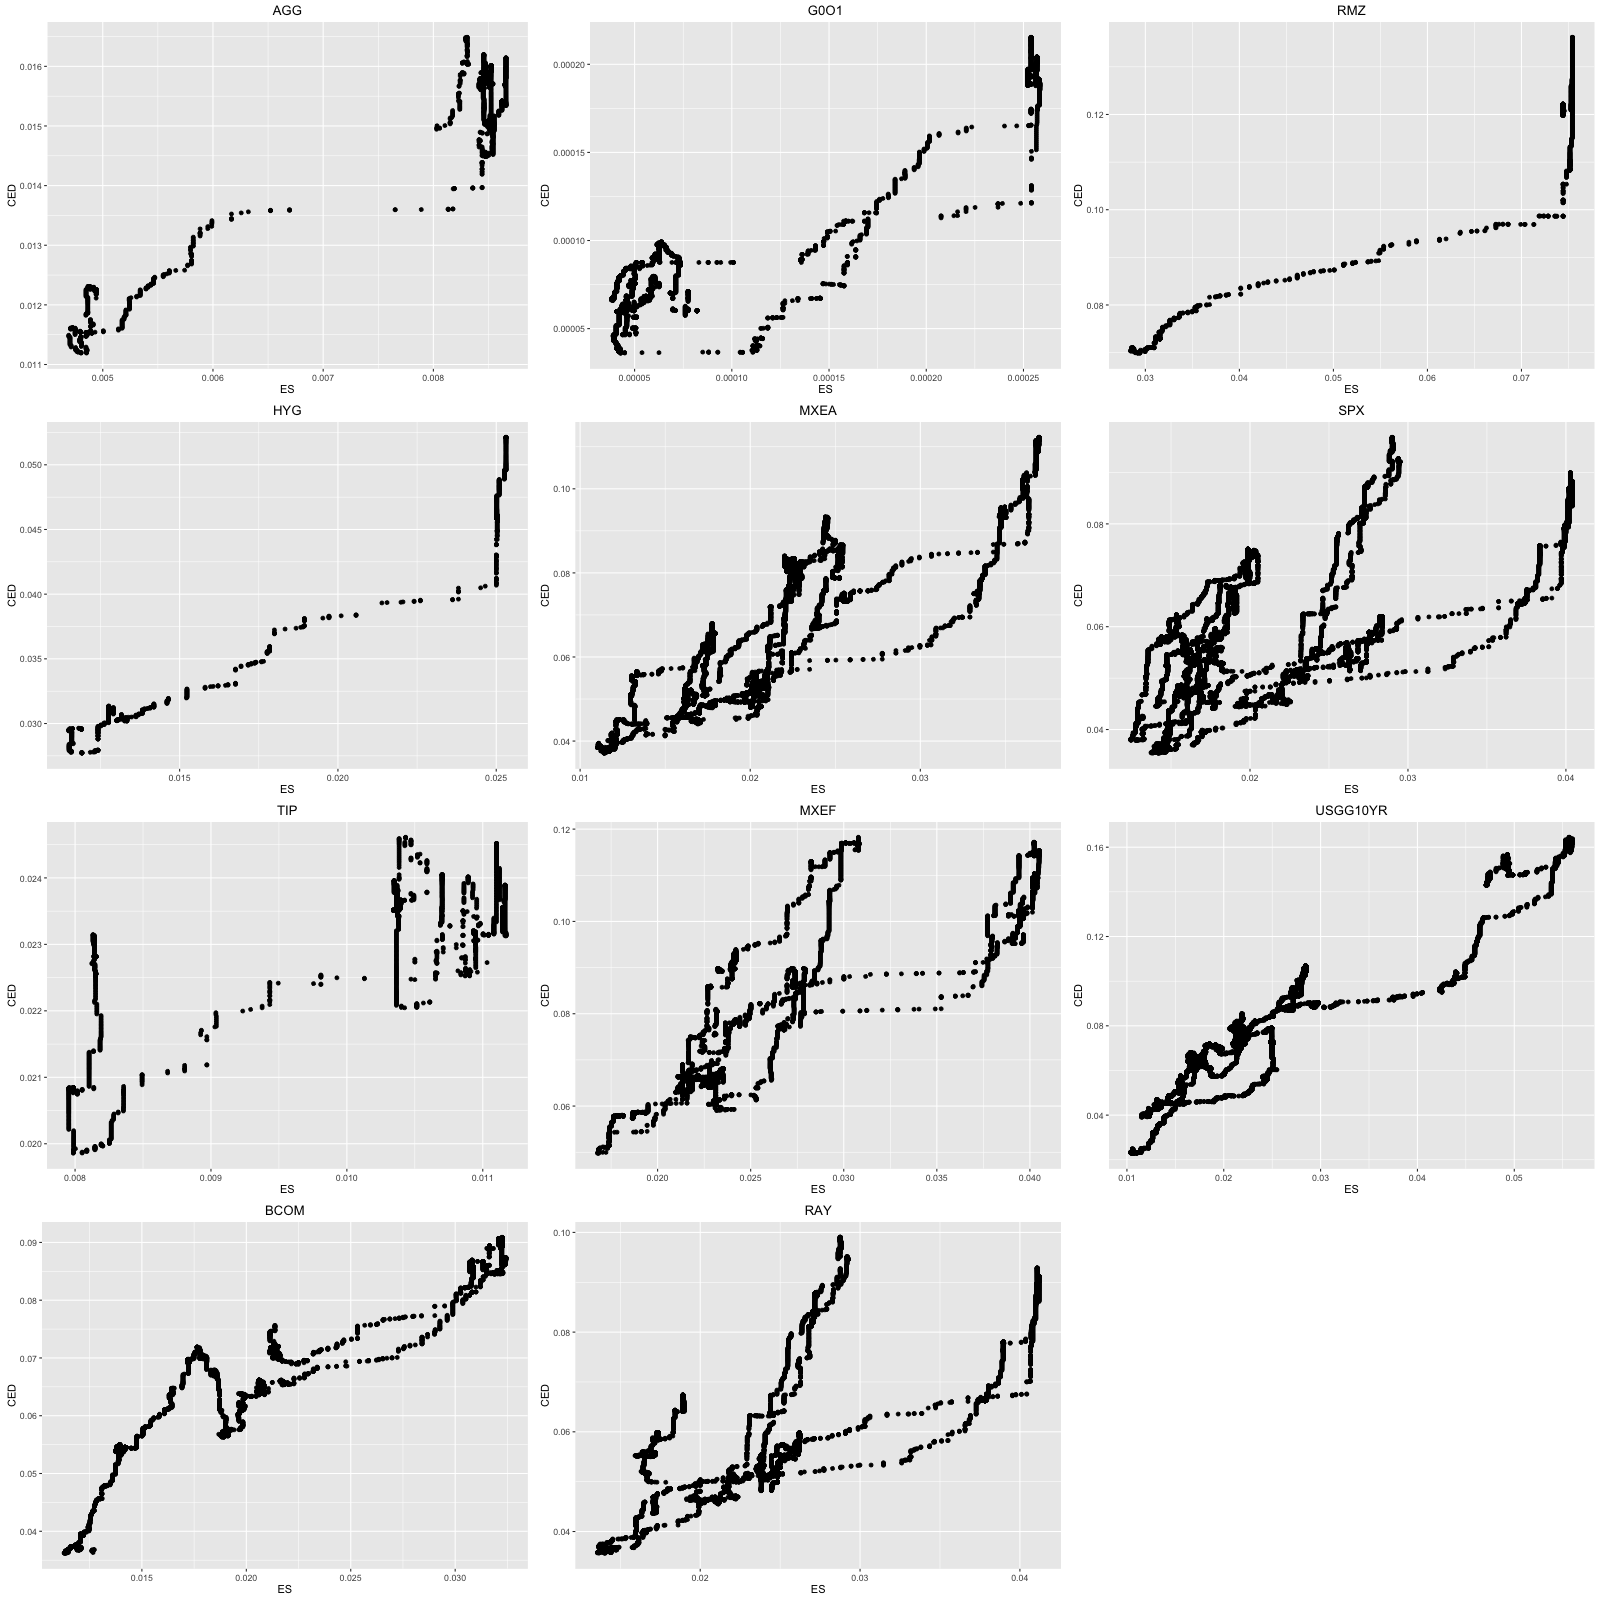
\includegraphics[width=15cm]{../results/CED_ES_3mon_5yr5yr}
\label{fig: CED_ES_3mon_5yr5yr}
\end{figure}

\begin{figure}
  \caption{First-order serial correlation calculated using AR(1) model versus VaR}
  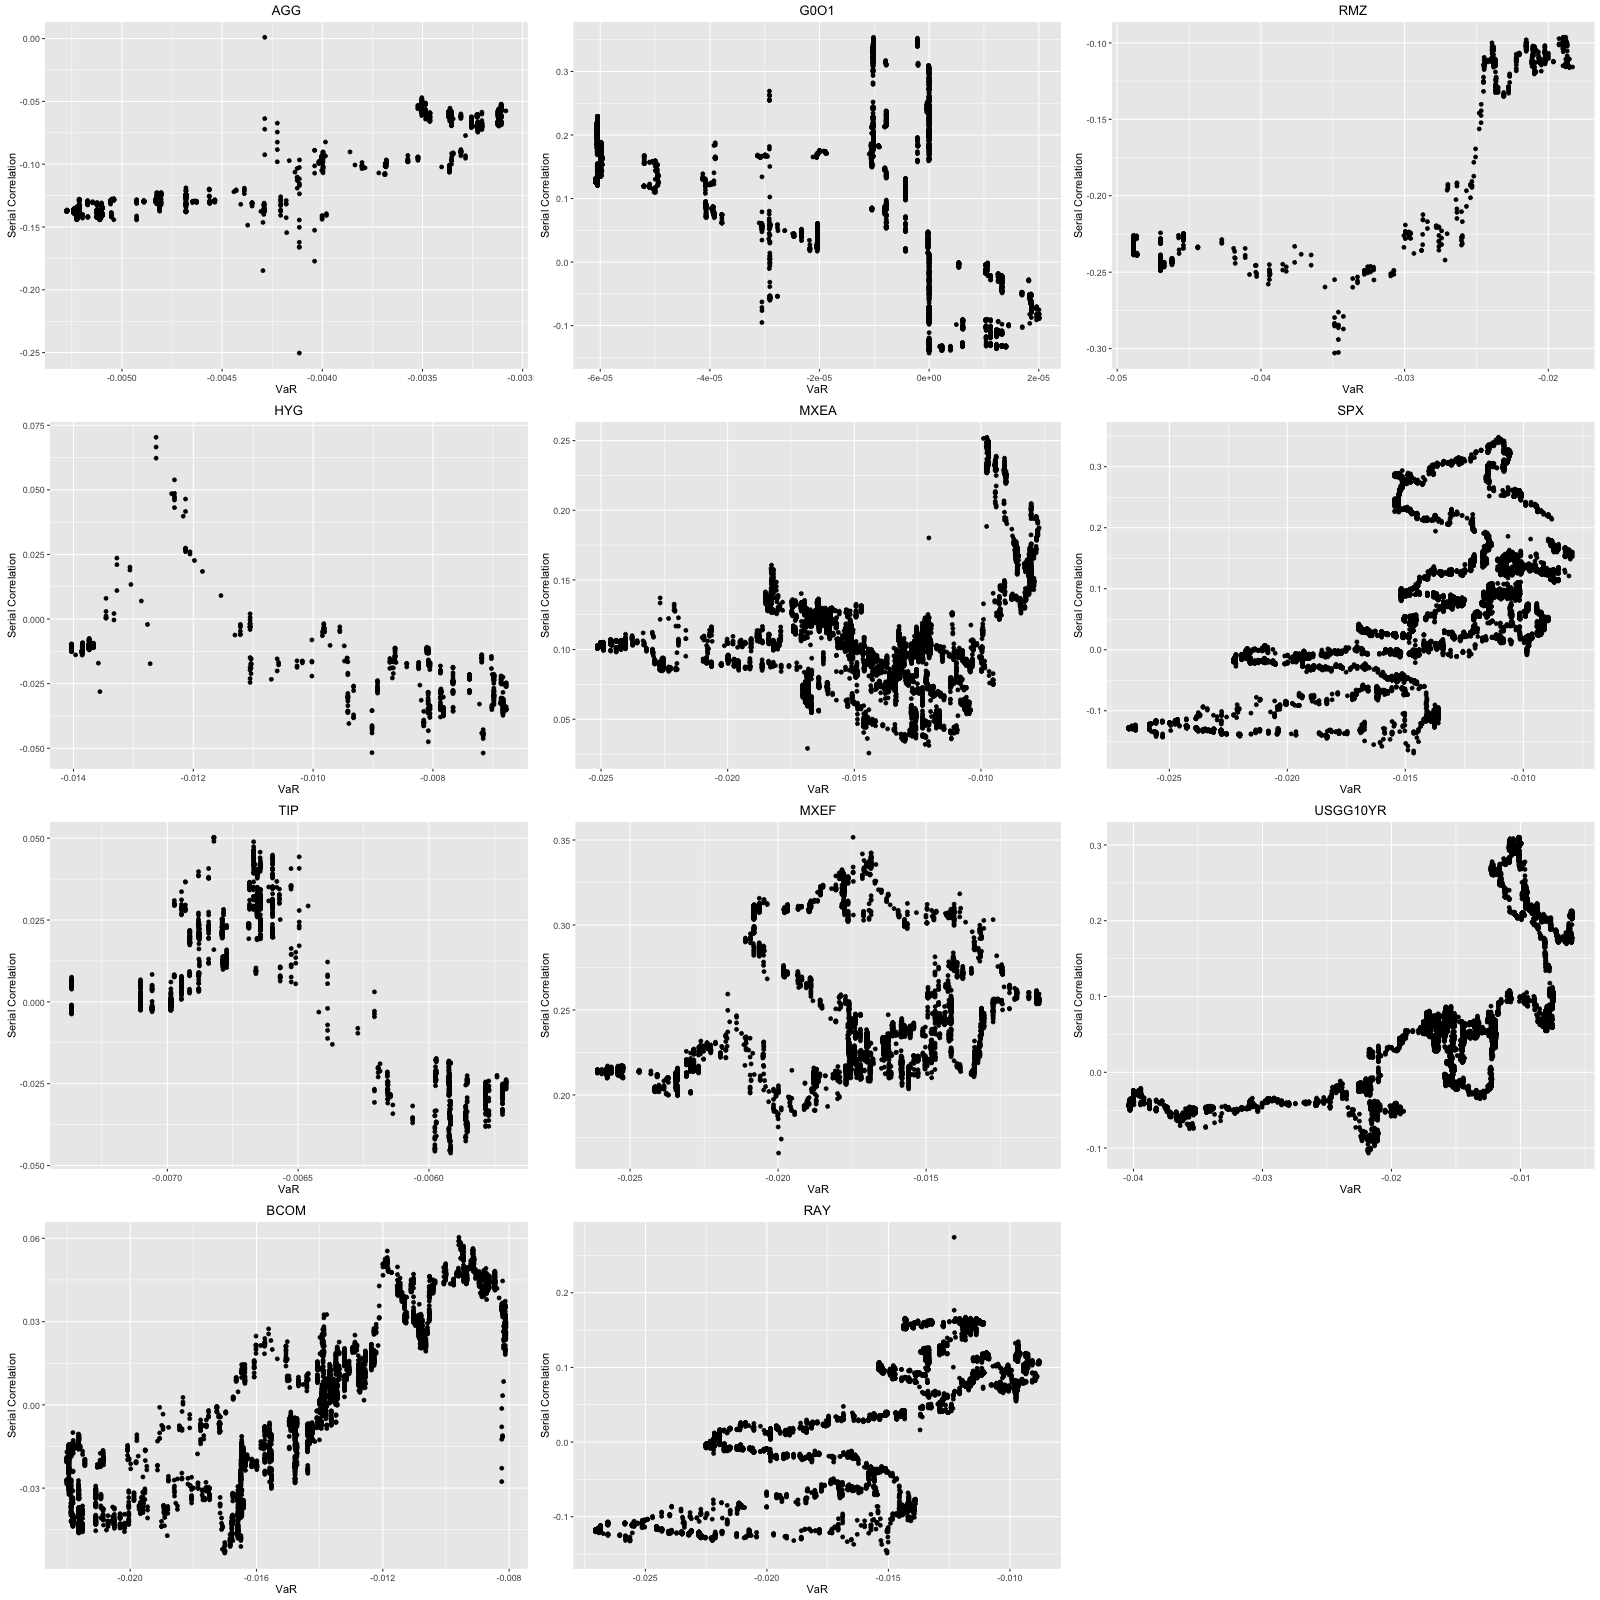
\includegraphics[width = 1\textwidth]{../results/SerCol-VaR5yrAR1}
  \label{fig:SerCol-VaR5yrAR1}
\end{figure}

\begin{figure}
  \caption{First-order serial correlation calculated using AR(1) model versus ES}
  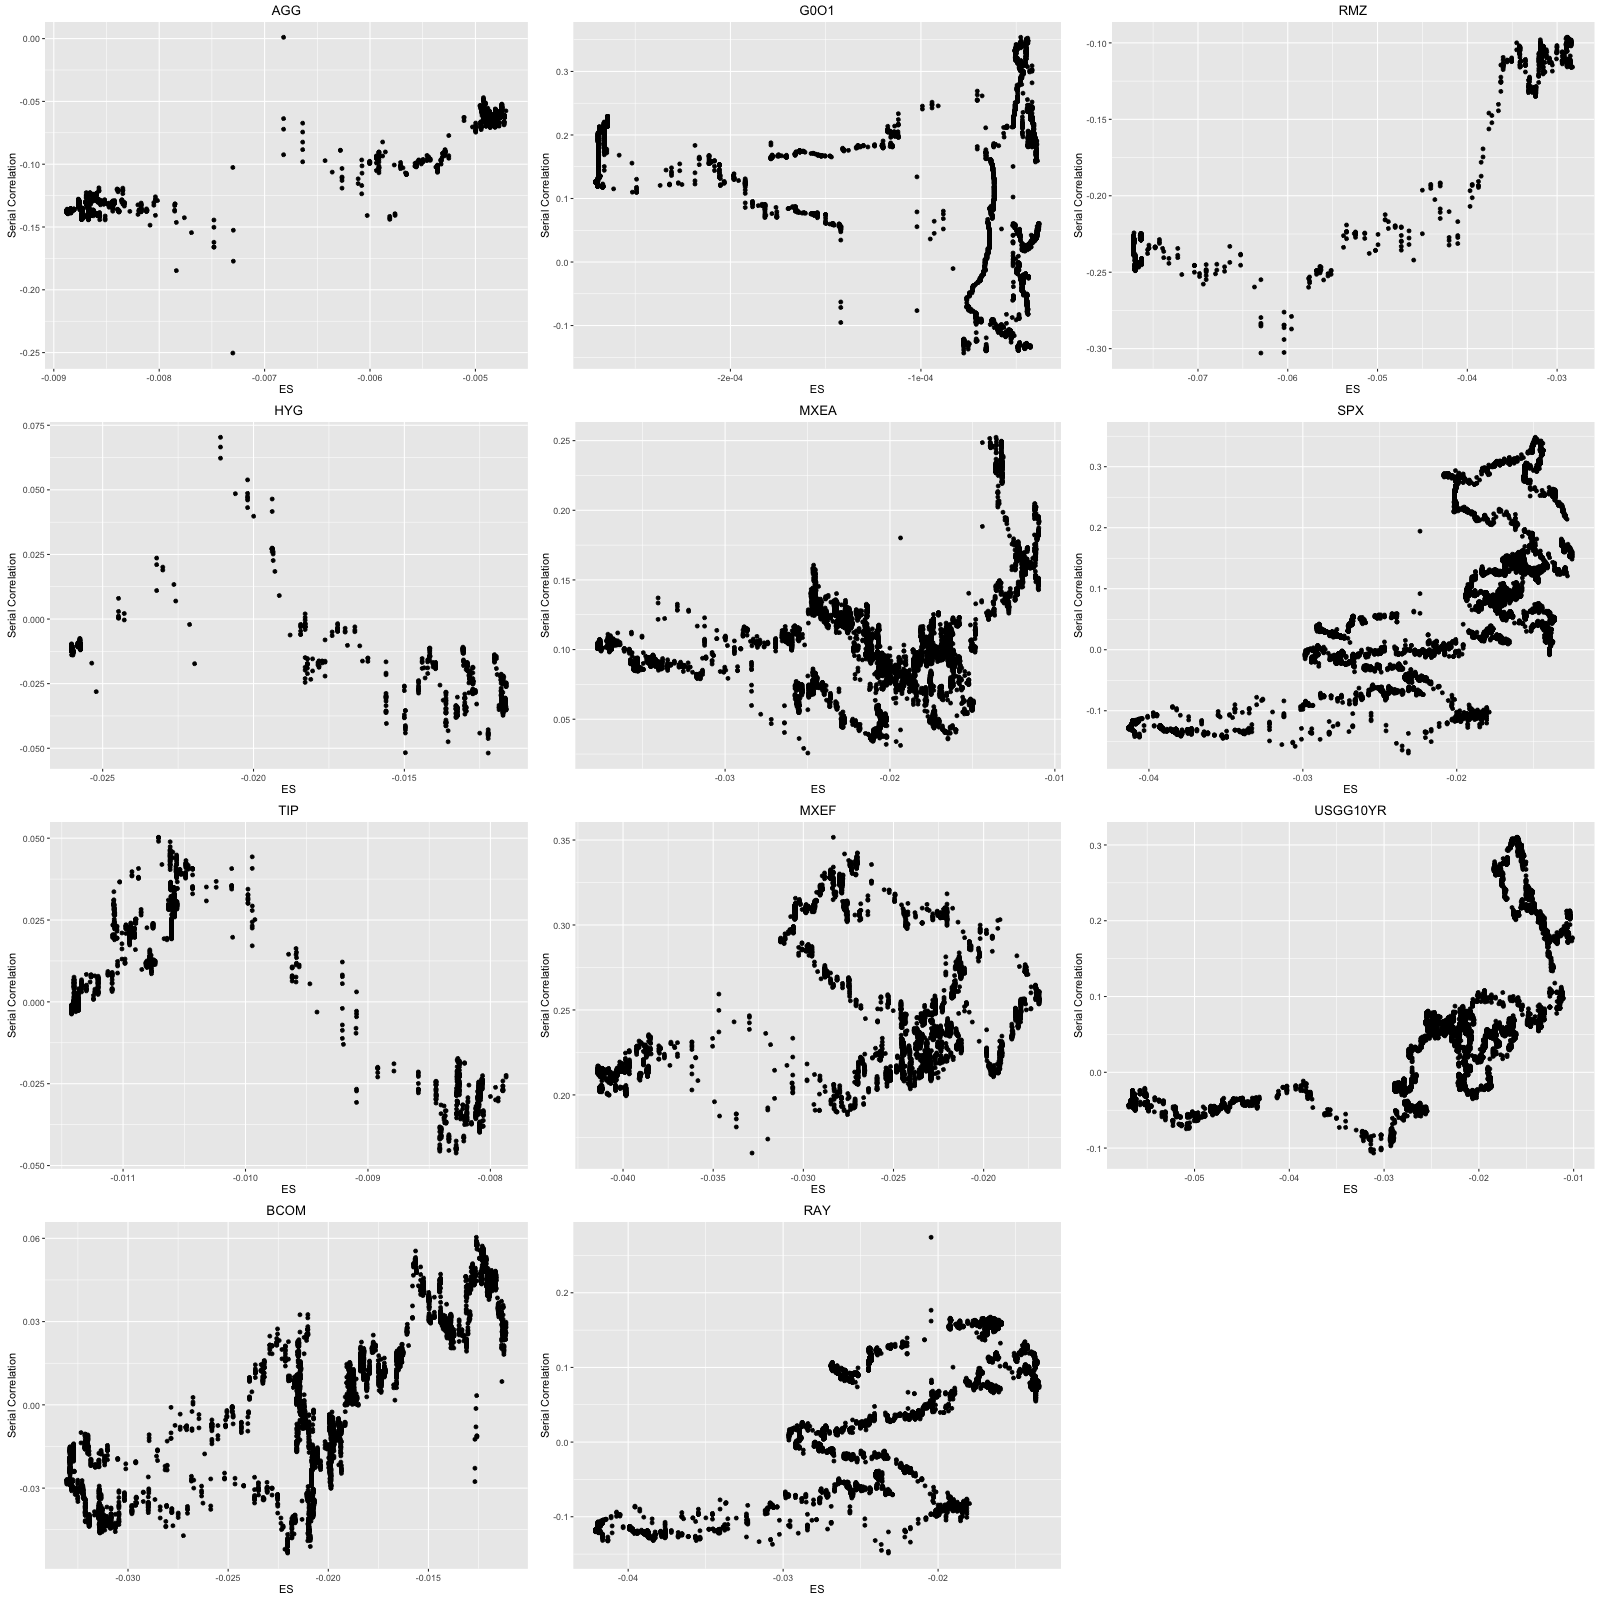
\includegraphics[width = 1\textwidth]{../results/SerCol-ES5yrAR1}
  \label{fig:SerCol-ES5yrAR1}
\end{figure}

\begin{figure}
  \caption{First-order serial correlation calculated using AR(1) model versus CED}
  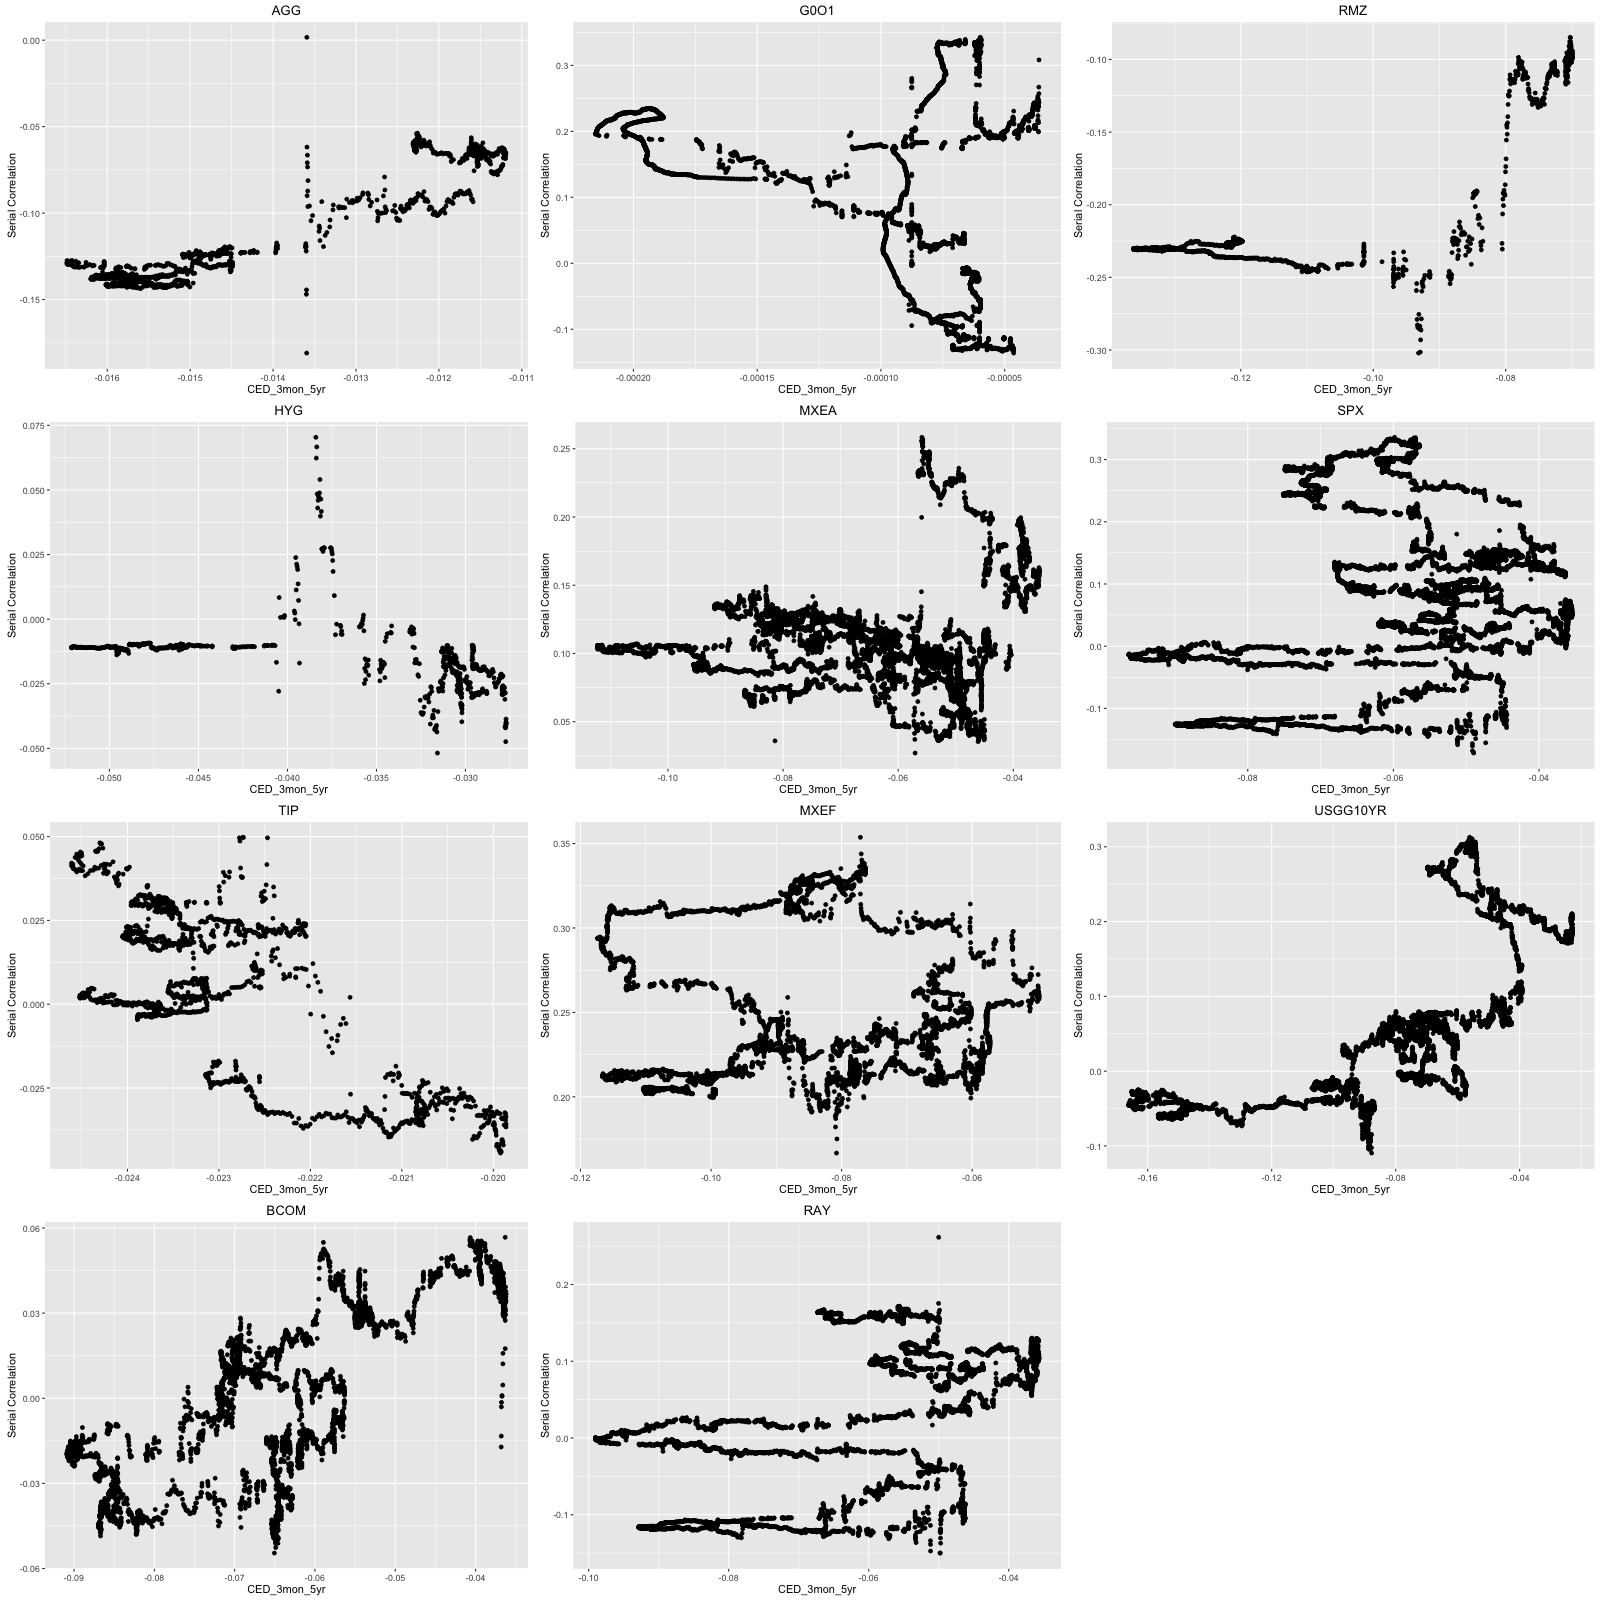
\includegraphics[width = 1\textwidth]{../results/SerCol-CED5yr3monAR1}
  \label{fig:SerCol-CED5yr3monAR1}
\end{figure}

\begin{figure}
  \caption{First-order serial correlation calculated using MA(1) model versus VaR}
  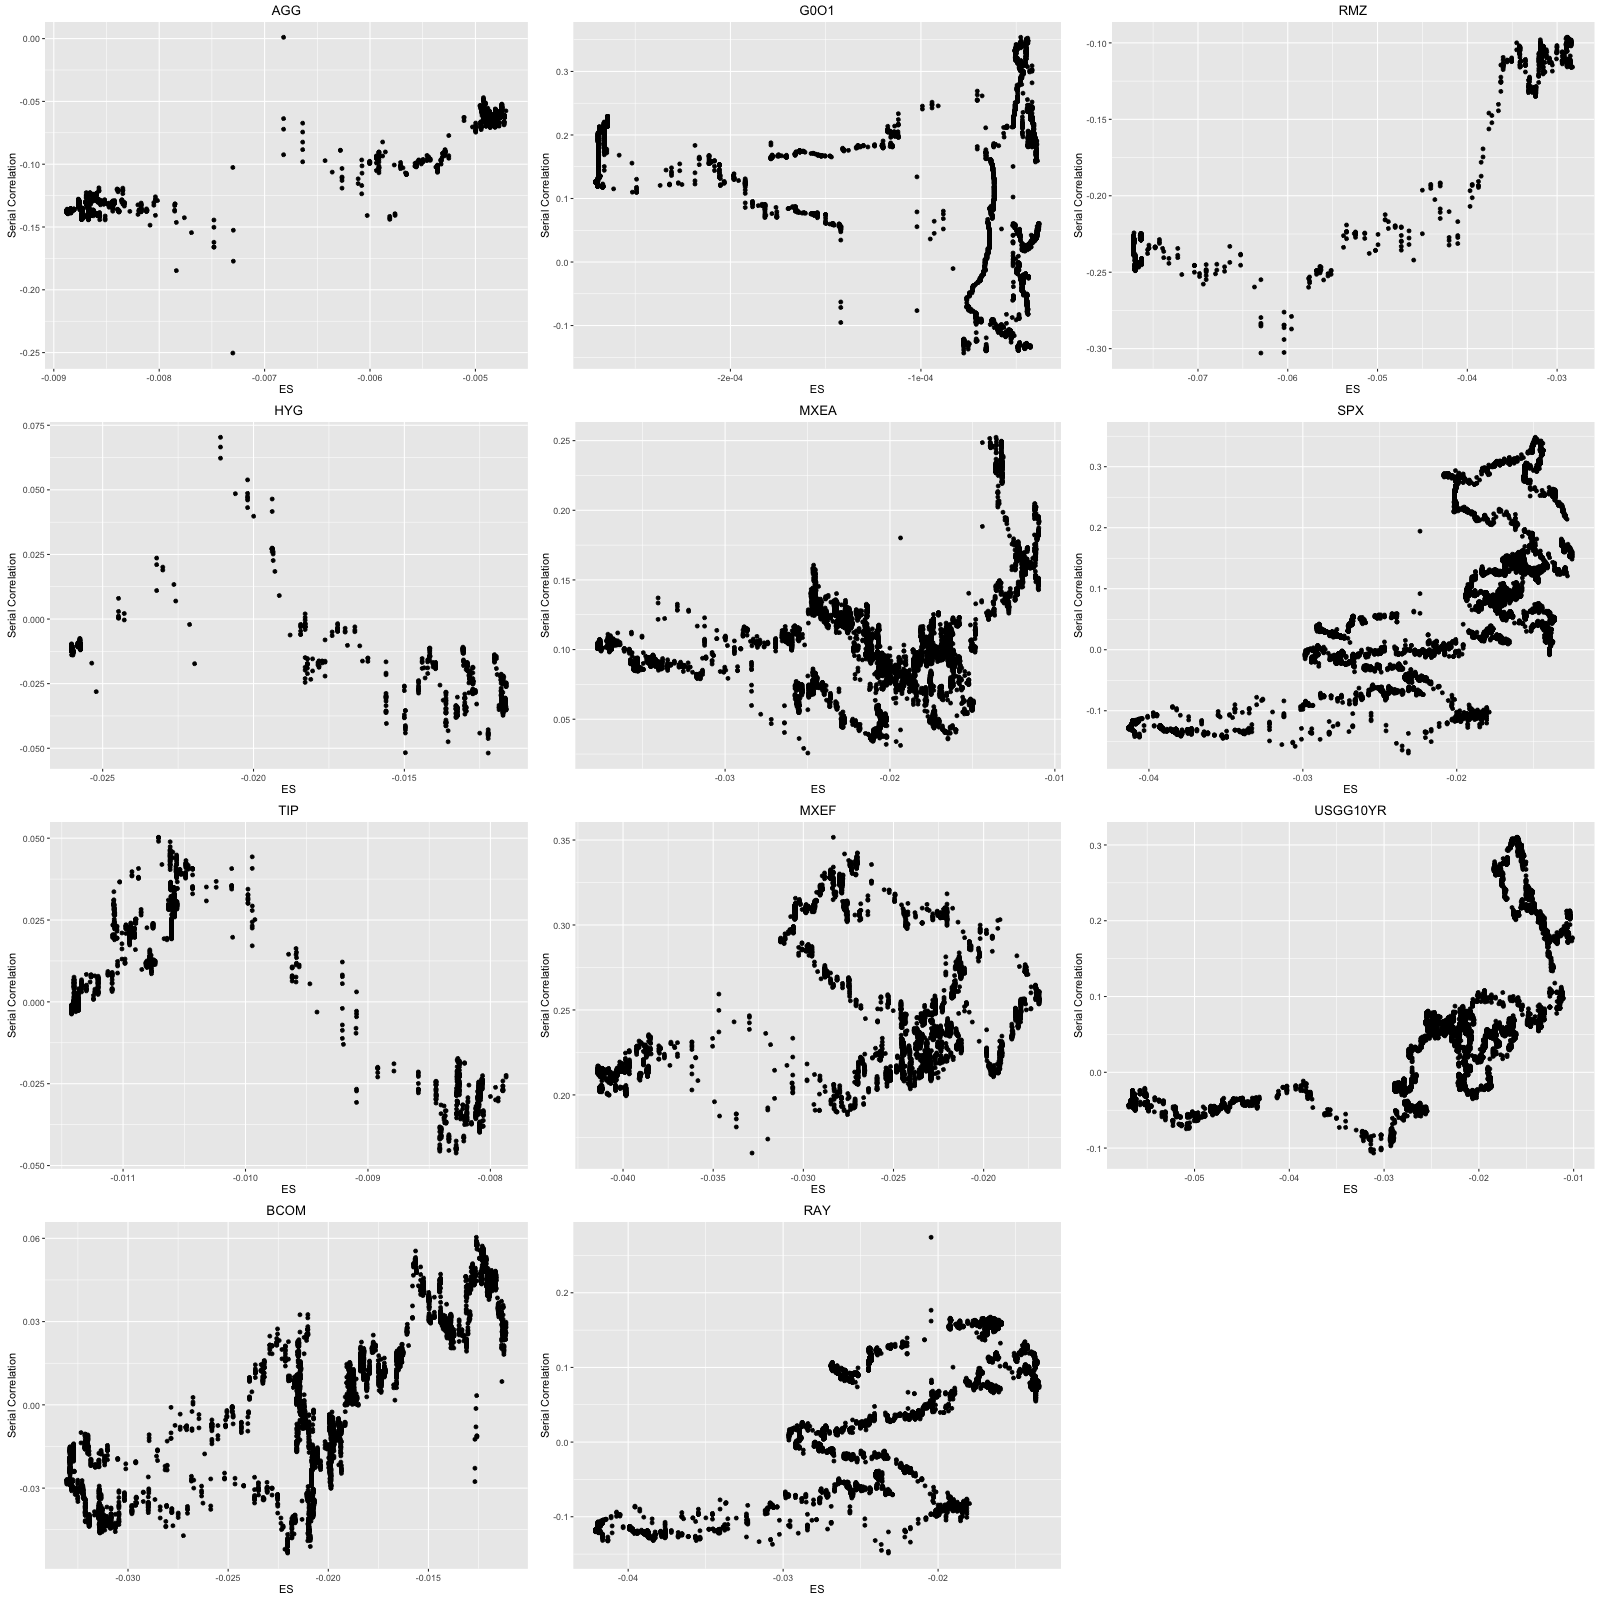
\includegraphics[width = 1\textwidth]{../results/SerCol-ES5yrMA1}
  \label{fig:SerCol-ES5yrMA1}
\end{figure}

\begin{figure}
  \caption{First-order serial correlation calculated using MA(1) model versus CED}
  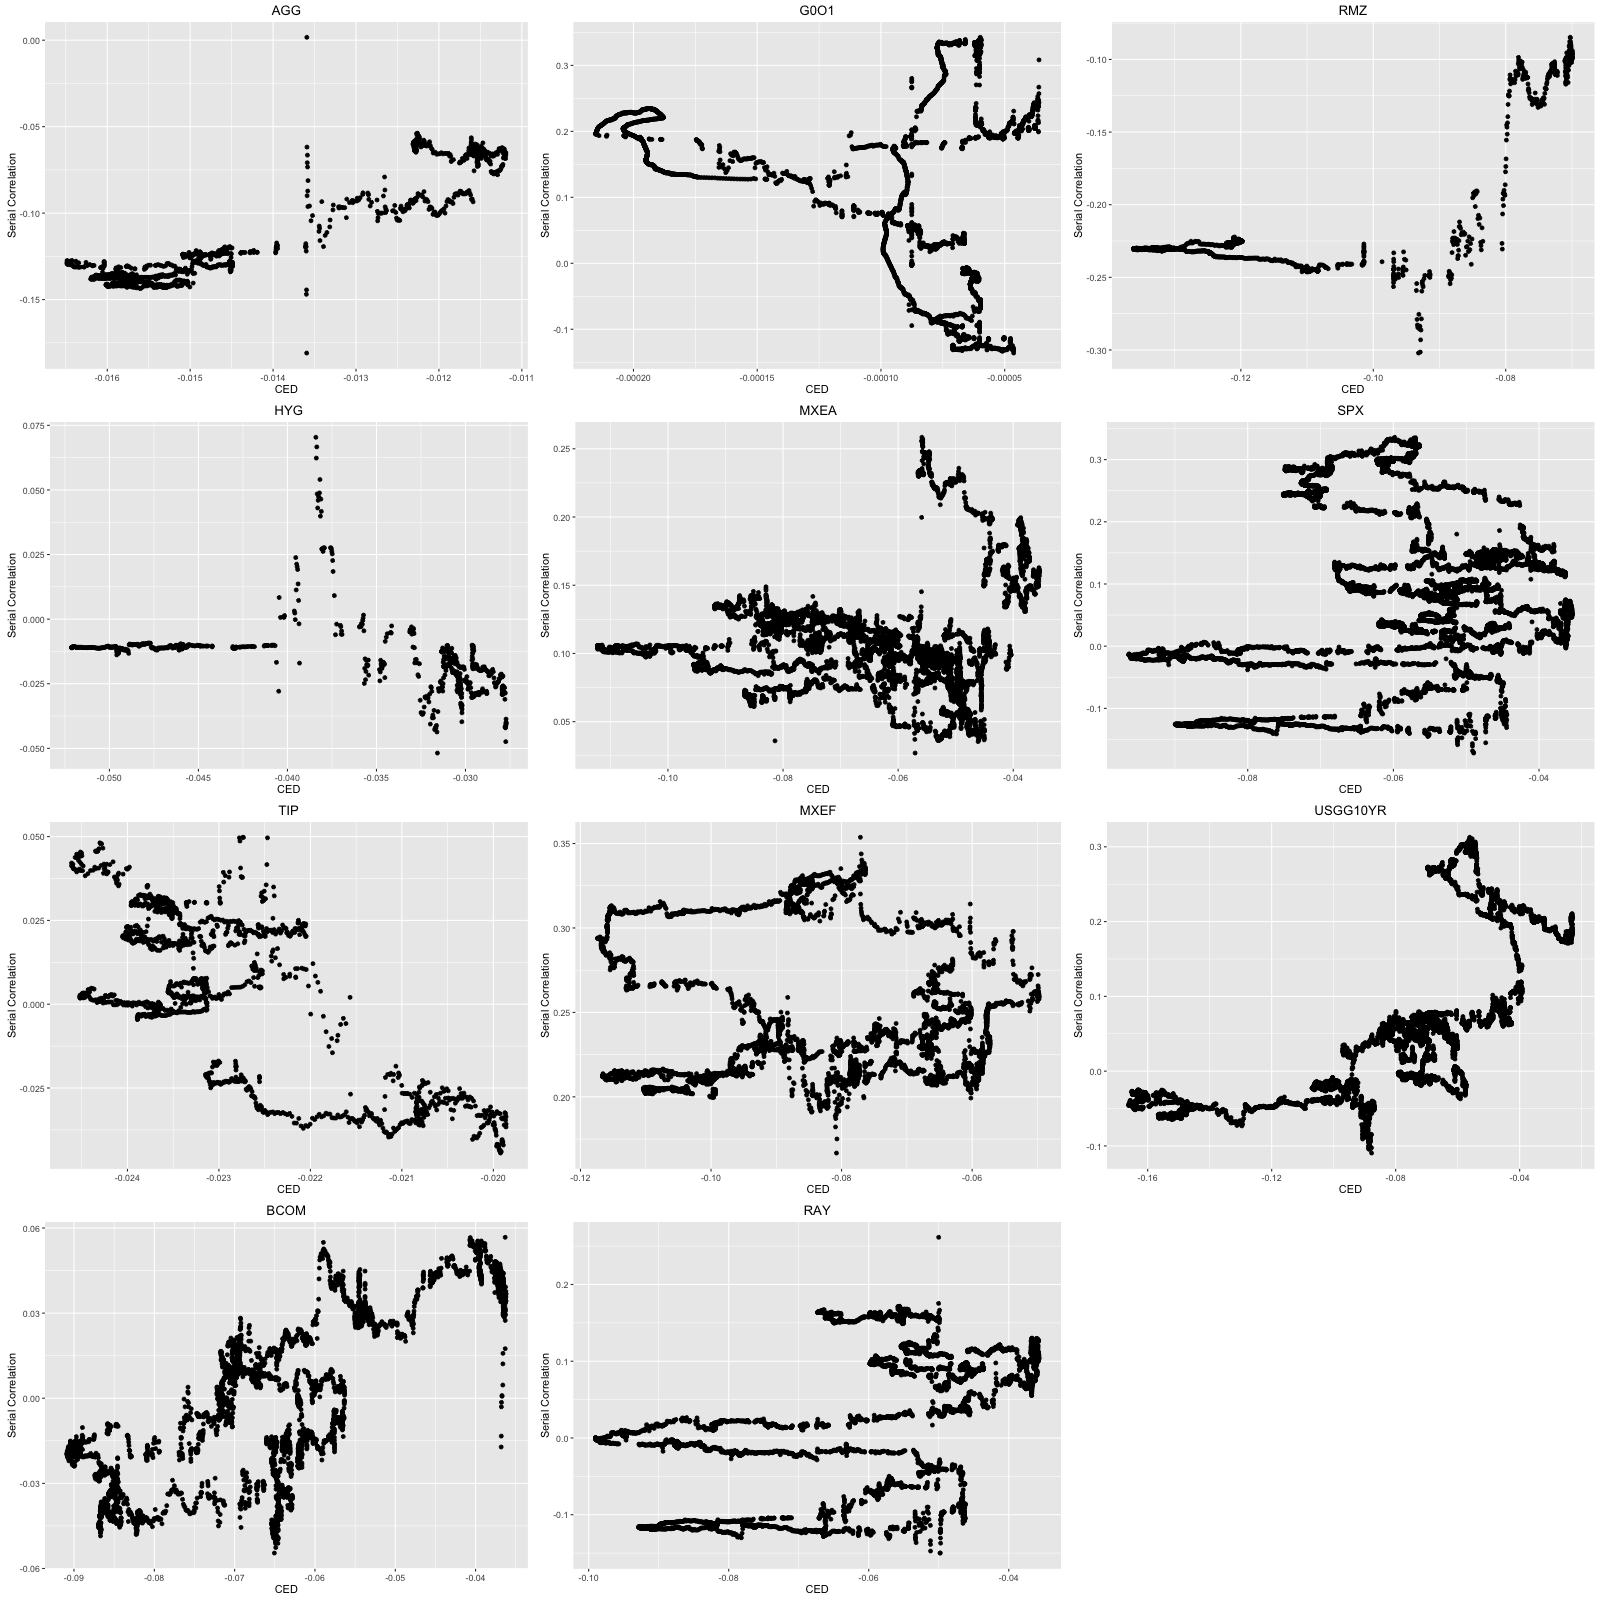
\includegraphics[width = 1\textwidth]{../results/SerCol-CED5yr3monMA1}
  \label{fig:SerCol-CED5yr3monMA1}
\end{figure}

\begin{figure}
  \caption{First-order serial correlation calculated using ARMA(1) model versus CED}
  \includegraphics[width = 1\textwidth]{../results/SerCol-CED5yr3monARMA11}
  \label{fig:SerCol-CED5yr3monARMA1}
\end{figure}

\clearpage

\bibliographystyle{unsrt}
\bibliography{analysis}

\end{document}
